\documentclass[10pt, oneside]{book}
% \documentclass[10pt]{book} %to print

\usepackage[utf8]{inputenc}
\usepackage[english]{babel}
\usepackage{microtype}
\usepackage{fancyref} % for refs
\usepackage{graphicx} % for including pictures
\graphicspath{ {./images/} }
\usepackage{amsmath} % useful for math
\usepackage{pgfplots} % for plots
\usepackage{booktabs} % good for beautiful tables
% packages for code
\usepackage{verbatim}
\usepackage{fancyvrb}
\usepackage{minted}
% useful packages
\usepackage{hyperref}
\usepackage{cleveref}
\usepackage{pdfpages}

% code style
% \newminted[code]{c}{frame=single, 
% framesep=2mm,
% baselinestretch=1.2,
% breaklines, 
% breakafter=d,
% linenos
% }

% EB: more compact
\newminted[code]{c}{frame=single, 
framesep=2mm,
baselinestretch=1,
fontsize=\footnotesize,
%fontsize=\scriptsize,
breaklines, 
breakafter=d,
linenos
}

\newminted[codebash]{bash}{frame=single, 
framesep=2mm,
baselinestretch=1.2,
breaklines, 
breakafter=d,
linenos
}

% EB: da usare al posto di verbatim quando le linee escono fuori dalla pagina
\newenvironment{mylongverb}{\begin{Verbatim}[xleftmargin=-2cm,fontsize=\footnotesize]}{\end{Verbatim}}

% \newcommand{\mycomment}[1]{\textbf{#1}}  % per vedere i commenti
\newcommand{\mycomment}[1]{}     % per rimuovere i commenti

% \author{Marco Perronet}
% \title{Linux Kernel: monitoring the scheduler by trace\_sched* events}

\begin{document}

\frontmatter
%TITLE
\begin{titlepage}
\includepdf[pages=-,pagecommand={}]{frontispiece/frontispiece.pdf}
\end{titlepage}

\tableofcontents
\listoffigures

\chapter{Abstract}
This thesis is about process scheduling and its implementation in the Linux kernel. Moreover, it covers other the kernel architecture and the event tracing, since they are a crucial component needed for kernel debugging. %write here an excitiong oneliner about what we're gonna do in the thesis
The focus is on illustrating the scheduler implementation in Linux kernel version 4.20.13 (released on 27--02--2019), as well as documenting scheduling-related events. In fact, both the kernel and the event tracing infrastructure are poorly documented.
Since the kernel and the tracing support are tightly related to each other, it is challenging to document the events without understanding how the scheduler works. Hence, most of the events are mentioned and explained on the fly, while discussing kernel concepts.

Examples of code are always provided, each piece of theory will have its implementation counterpart shown and explained.
Most of the concepts are very easy to visualize once the code is split into its most significant parts
and then dissected line by line; however, this is not an internals manual for development. 
This thesis should be considered a guide. It's meant for people who are curious about the inner workings of the kernel
but have never looked too much into it, its goal is to give interesting insights about the architecture of operating systems.
The only prerequisite is to have some experience with C and know the very basics of GNU/Linux and operating systems.

All references to the source code are from kernel version 4.20.13, the latest stable version at the time of writing. When discussing architecture dependent code it will be assumed that the architecture is x86. In the code, every comment spanning over multiple rows (\verb|/*...*/|) is written by the kernel developers, my comments will always be inline (\verb|//|).

%Explain how the thesis is structured
In the first part I will give a brief overview of the kernel and then explain some basic scheduling concepts.\\
\dots (will write this at the end)
\dots\\
Here is a useful tool to quickly look up mentioned kernel functions for yourself \texttt{elixir.bootlin.com/linux/v4.20.13/source}. Another alternative is to download the whole source code from \texttt{kernel.org}, which is needed if you want to compile and load it. 


\mainmatter

\chapter{Basics of Linux kernel} %Capitolo in comune
\label{ch:introduction}

\section{Operating Systems}
\label{sec:os}
The operating system (OS) comprises the software intended to manage the hardware resources and the \textit{application software}, which performs specific, high-level tasks. The application software, which is the larger part of the OS, is made of utility programs and any other software with which the user interacts directly. These programs are not part of the core OS. Rather, they are necessary to do anything useful. The operating system acts as an intermediary between the user and the machine by abstracting away the hardware, which makes interaction easier: this is why almost every computer runs an operating system.

It can be argued that the OS is not strictly necessary because it's possible to execute a program without loading an OS: this is referred as \textit{bare metal programming} and it is common in small size embedded systems. Because there is no operating system (which means no file system, memory management or any useful application such as compilers), programs cannot be written on the system itself. Instead, the program is written on another machine with an operating system, then compiled with a cross-compiler, which compiles for a target architecture different from the one it is running on. Finally, the compiled binaries are loaded at boot time on the target embedded system. This is the opposite of what we are used to doing on our laptops/desktops: to be able to reprogram the machine as it is running, by writing and compiling our program with \textit{application software} designed to edit text and compile code. Thus, an operating system greatly simplifies interaction with the machine by offering a platform for the user and, at a higher level, by making general-purpose computing possible.
%There are also OSes for embedded systems called \textit{real-time systems}, but we will focus only on general-purpose OSes. 

Windows, MacOS, iOS, Android\dots\   Most of us are familiar with these operating systems. Besides the platform on which they run, they are all general-purpose and their goal is the same. What really changes among them is the architecture and philosophy in their design. At a macroscopic level they differ in kernel design approach (monolithic kernel vs.\ hybrid kernel). This is explained later in Section \ref{img:monolithic}. At a microscopic level, there is literally not much to see because the code of most OSes is closed, so it's impossible to see the implementation differences with Linux. This leads us to one of the peculiarities of Linux: it's completely open source and community developed. Besides ethical matters, which are not discussed here, this means that it's possible to study the code and get a full understanding of operating systems. In fact, before Linux, there was no way to see how operating systems work in practice. The only option was to study them from textbooks in order to implement your own kernel, which is exactly what Linus Torvalds did.

As stated earlier, a key component of an OS is ``the software intended to manage the hardware resources'': this is what we refer as the \textit{kernel}. Dennis Ritchie, among the inventors of Unix and C, also called it the ``Operating system proper''\cite{ritchie}, which most likely means ``The component that is the actual operating system''. On the one hand this definition makes sense, because the low level tasks performed by the kernel are essential (and also because it's the most difficult component to develop). But on the other, without application software the kernel is useless. In such scenario, the kernel is loaded at boot, then it initializes and starts running, and then there is nothing but a black screen because there is no other program to start. It's clear that the kernel is not an operating system by itself, but what Dennis meant is that when we think about the core architecture of an OS, we think about the kernel. An engine is indeed useless without the rest of the car, but does that make the other components as important as the engine, where all the complexity resides? Despite the application software being the largest part of the OS; it is within the kernel that the hardest engineering challenges are found, which makes it the most interesting---and difficult---part to understand and analyze.

\section{A general overview} 
\label{sec:general}
The kernel's job is to manage hardware resources, which means handling all interactions with the CPUs, the memory hierarchy and the I/O devices. More specifically, the kernel needs to respond to I/O requests, manage memory allocation and decide how the CPU time is shared among the demanding processes. To achieve this, it has access to all resources in the system, which is needed to make the most out of the hardware. Its performance is what makes the difference between a fast or a slow operating system. This critical role requires a protection mechanism to ensure the stability and the security of the whole system. This is achieved by separating kernel code and user application code. In practice, depending on the configuration settings at compile time, what happens is: 
\begin{enumerate}
    \item The kernel binary image is loaded in RAM in a memory area which can start from a low or high address.
    \item A pre-defined slice of RAM next to that memory area is reserved to the kernel. 
    \item The remaining part of the memory is accessible to the user.
\end{enumerate}
These two portions of the address space %of RAM
are called kernel space and user space. The former is a reserved area dedicated to critical system tasks and it's protected from user access, the latter is the area where system utilities and user programs run. This memory partitioning makes sure that kernel and user data do not interfere with each other. Also, it is a security measure to prevent that a malfunctioning or malicious user program may affect the entire system.

\subsection{System calls}
By extension of this design, the interaction with the user space is regulated with a privilege system. Each process can run either in user mode or kernel mode. Processes running in user mode can access privileged kernel functionalities through special gates in a pre-defined and controlled manner. These gates are implemented as functions called \textit{system calls}, which serve as APIs between user and kernel space. When a user process performs a system call
\begin{enumerate}
    \item it temporarily executes in kernel mode, 
    \item it performs tasks that require a high privilege, and finally
    \item it switches back to low privilege.
\end{enumerate}
This mechanism exploits the availability of hardware functionalities.
For example, in the x86 architecture 2 bits in the code selector (\verb|cs|) register indicate the current privilege level (CPL) of the program that is running on the CPU. This value is 0 or 3, respectively, for kernel and user mode and each system call changes this value temporarily. 

\begin{figure}[ht]
  \centering
  \includegraphics[width=.75\textwidth]{images/userspace_kernelspace.png}
  \caption{Kernel space (in red) and user space (in green and blue)}
  \label{img:userspace_kernelspace}
\end{figure}

Very often, useful operations in the system require privileged services provided by the kernel. For example, even an extremely simple shell command such as \verb|echo| performs dozens of system calls, which are reported below as listed by the command \verb|strace -wc echo|
\begin{Verbatim}
% time     seconds  usecs/call     calls    errors syscall
------ ----------- ----------- --------- --------- ----------------
 29.57    0.000514         514         1           execve
 17.03    0.000296          33         9           mmap
 11.62    0.000202          67         3           brk
  8.52    0.000148          37         4           mprotect
  7.19    0.000125          25         5           close
  6.10    0.000106          35         3           open
  5.93    0.000103          26         4           fstat
  5.58    0.000097          32         3         3 access
  2.82    0.000049          49         1           munmap
  2.24    0.000039          39         1           write
  1.84    0.000032          32         1           read
  1.55    0.000027          27         1           arch_prctl
------ ----------- ----------- --------- --------- ----------------
100.00    0.001738                    36         3 total
\end{Verbatim}
System calls can be called in user space applications directly, through assembly, or indirectly, by calling wrapper functions from the C standard library (\verb|glibc|), as shown in Figure \ref{img:userspace_kernelspace}. 
\begin{code}
// Two different ways of calling open/close through glibc wrapper functions 
// SYS_open and SYS_close correspond to the syscall numbers
int fd = syscall(SYS_open, "example.txt", O_WRONLY);
syscall(SYS_close, fd);
fd = open("example.txt", O_WRONLY);
close(fd);
\end{code}
Calling through assembly means filling the right CPU register with the syscall arguments and then using a special assembly instruction. On x86 machines it is required to fill the \verb|EAX| register with the system call number (by a \verb|mov| assembly instruction) and then invoke the interrupt 128 (by the instruction \verb|int 0x80|). Modern processors may use a different one. This is what will happen upon its execution:
\begin{enumerate}
    \item Interrupt number 128 (=\verb|0x80|) is released. In Linux, it corresponds to a system call interrupt. 
    \item The process execution is suspended and the control passes to the kernel (kernel mode), which will look up the entry 128 in the \textit{interrupt vector table}. This table simply associates interrupt numbers with their handler: a function that gets executed when the interrupt happens.
    \item The corresponding handler is executed: this function copies the syscall number and arguments from the registers onto the kernel stack. It will then look up in the \textit{system call dispatch table} the handler corresponding to the syscall number and call it with the correct arguments like any normal C function, because the arguments are now located on the kernel stack.
    \item The system call is finally executed and the return value is stored in a general-purpose data register.
\end{enumerate}
Registers are used to pass the parameters because this way it's easier to get them from user to kernel space. It is intuitive that such a procedure to invoke system calls is architecture dependent. For this reason, \verb|glibc| wrappers are always used: they internally execute the assembly code that we just illustrated and do it differently for each architecture.
%(you can write assembly into C source code, more on this later).
Calling wrappers is also very safe since it avoids to accidentally fill the wrong registers or miss the right number of arguments.
%and, moreover, most syscalls have a wrapper so there's no reason to write assembly for them.
It's important to note that the kernel can protect itself against invalid syscall arguments in registers. This is crucial since, as we saw, syscalls are easily called from user space directly by executing the proper assembly instructions.

\subsection{A different kind of software}
The separation between kernel/user space and the fact that we are working at such low level makes the kernel a very peculiar piece of software. One of its properties is that there is no error checking, this is because the kernel trusts itself: all kernel functions are assumed to be error-free, so the kernel does not need to insert any protection against programming errors\cite{cesati}. Instead, what the kernel does is to use assertions to check hardware and software consistency; if they fail then the system goes into \textit{kernel panic} and halts. Later on in Section \ref{ch:events_documentation}, it is shown an example of code where the \verb|panic()| routine is called. The choice of checking assertion (and possibly going to kernel panic if something went wrong) is that since the kernel controls the system itself, error recovery and error correction is very hard and would take a huge part of the code. Another way of thinking about it, is that there is no meta-kernel that handles kernel errors. Of course programming or hardware errors can (and will) still occur: when this happens the offending process is killed and a memory dump called ``\textit{oops}'' is created. A typical example of this is when the kernel dereferences a NULL pointer: in user space this would cause a \textit{segmentation fault}, while in the kernel it will generate an oops or in the worst case go directly into panic. After this kind of event, the kernel can no longer be trusted and the best thing to do would be to reboot, because the kernel is in a semi-usable state and it could potentially corrupt memory. Furthermore, a panic in this state is more likely to happen. %oops count after the first one?
Possibly, the user experiencing the kernel panic may also inform the kernel mantainers.

% Ricordare di mettere parentesi quando si citano funzioni
Another peculiarity of the kernel is that it uses its own implementation of the functions in the standard C library. For example \verb|printf()| and \verb|malloc()| are implemented as \verb|printk()| and \verb|kmalloc()|. There are different reasons for this choice, one of those is that the C standard library is too big and inefficient for the kernel. Another reason is that implementing your own functions gives more freedom because they can be customized for their purpose in the kernel. Memory allocation in user or kernel space is very different, so the \verb|kmalloc()| implementation is very specific. For instance, kernel data structures need a contiguous physical memory segment to be allocated, while regular user space allocation doesn't have this restriction. Furthermore, \verb|printk()| writes its output into the kernel log buffer (that you can read by using the \verb|dmesg| command in user space); this is very different from \verb|printf()| that writes on standard output.

\subsection{User and kernel stacks}
As stated earlier, the memory management is different in kernel/user space.
The same applies to the execution. Every process in the system has two stacks, located respectively in user and kernel space, and it will use one of the two while executing in the corresponding privilege mode. x86 CPUs automatically switch stack pointers when privilege mode switches occur, which usually happens for syscalls. The user space stack can potentially be very big, with a very high limit (8MB on my machine, but it can be increased), and even though it's initially small it can allocate more physical memory as it needs it: this mechanism is called ``\textit{on-demand paging}''. The kernel stack, unlike the user stack, cannot expand itself and it has a fixed size of two pages. Since, 32-bit and 64-bit systems have 4KB and 8KB sized pages, then the kernel stack size is of size 8KB or 16KB, respectively. These two pages must be allocated contiguously, which can cause memory fragmentation for long system uptimes as stacks get deallocated. In other words, it becomes increasingly hard to find two physically contiguous unallocated pages as the OS runs for a long time. For this reason, in the past efforts were made to reduce the stack size to one page, which would eliminate fragmentation, but after many stack overflows the standard settled on two pages.

This leads us to an interesting example of the kernel trusting itself: it makes the strong assumption that the stack will never overflow: \textbf{no protection against it is in place}. So what happens if it overflows? First, it will corrupt the \verb|thread_info| data structure, which is the first data that the stack encounters along its path (Figure \ref{img:stack}). This will make the process nonexistent for the kernel and cause a memory leak. Next, the stack can overflow outside of the address space and silently corrupt whatever kernel data is stored; the best case scenario here would be a kernel panic to prevent any further memory corruption. Another natural question might be ``why are kernel stacks so small?'' and the answer is simple: first, to use a small amount of kernel memory, and secondly, because of fragmentation. The bigger is your data structure in contiguous physical memory, the more it is hard to allocate. It is expected that any process stays in kernel mode for a small amount of time, so it should use a very small portion of the stack. A consequence of small stacks is that very few recursive functions are used to avoid long call chains and minimize stack usage; the same is true for big static allocations on the stack. %check this

\begin{figure}[ht]
\includegraphics[width=\textwidth]{images/stack}
\caption{The kernel stack inside its small address space of two pages, it grows downward towards low memory.}
\label{img:stack}
\end{figure}

It's important to note that there are special processes called \textit{kernel threads} that do not follow this pattern of kernel/user stack. Kernel threads perform a specific system task, they are created by the kernel and they live exclusively in kernel space, never switching to user mode. Their address space is the whole kernel space and they can use it however they want. Besides this, they are normal and fully schedulable tasks just like the others. An example of a kernel thread is \verb|ksoftirqd|: there is always one for each CPU and their job is to dispatch interrupt requests. As a side note, the name stands for ``Kernel Software Interrupt ReQuest Daemon'', many kernel threads follow a similar naming convention. 
%Maybe mention per-CPU interrupt stacks? (for interrupt handlers)
%Interrupt stacks - To rectify this problem, the kernel developers implemented a new feature: interrupt stacks. Interrupt stacks provide a single per-processor stack used for interrupt handlers. With this option, interrupt handlers no longer share the kernel stack of the interrupted process. Instead, they use their own stacks. This consumes only a single page per processor.

\subsection{A monolithic design}
\label{sec:monolithic}
There are fundamentally different design approaches in kernel development. We can see these as a spectrum, where on one end there is the \textit{monolithic kernel}, and on the other one the \textit{microkernel} (or $\mu kernel$). The choice depends on how many services are located in kernel space: while in monolithic design every service is in the kernel itself, microkernels strive to reduce as much as possible the code running in kernel space. This is done by moving most services in user space, while keeping only essential primitives in the kernel (Figure \ref{img:monolithic}).

\begin{figure}[ht]
\includegraphics[width=\textwidth, keepaspectratio]{images/monolithic.png}
\caption{The most popular kernel designs and their differences}
\label{img:monolithic}
\end{figure}

These services are implemented as \textit{servers}, and communication between the servers, applications, and the kernel is based on message passing. As in classic client/server approach, applications send requests to the servers, which can in turn request services to the kernel or satisfy the request directly. Because of this design choice, the system relies heavily on \textit{Inter-Process Communication} (IPC), which can be achieved in different ways: in this case, there are actual messages being passed between processes. Even if they are part of the core architecture, the servers are user processes and run in user space just like the other user processes, though they get higher privileges.

By reducing the code running in kernel space, there is less risk for bugs. Because the trusted codebase is very small, there is no need to make big assumptions like in monolithic kernels. As stated before, a bug in the kernel can bring down the entire system, but in microkernels bugs are contained. For example, if the networking service crashes, then we can just restart it since it's just a user process; in a monolithic environnement, this problem would have crashed the entire system: this is one of the biggest flaws of the monolithic design. A small trusted codebase also means more portability because all the achitecture dependent code is concentrated in the small kernel. The actual operating system is built on top of it, so it would be possible to implement it in a more high level language, while only the primitives in the kernel must be ported. Conversely, in a monolithic kernel, many functions must be rewritten for each architecture: in Linux, the folder for architecture dependent code (\verb|arch|) is the second biggest folder and it represents 8\% of the code.

Another direct consequence of the shift of the code in user space is that microkernels are more easily maintainable. Development is easier because most of the code runs in user space, so the usual restrictions for kernel code are not present: for example, it would be possible to make use of \verb|glibc|. Furthermore, testing can be done without rebooting the system: just stop the service, recompile the code and then start it again. On a monolithic system, not only it's needed to recompile the whole kernel, we must also reboot in order to load the image again. And if this new image doesn't work, then we must reboot again with the working image. In practice, this is always done in a virtual machine in order to test more efficiently, but it's still a tedious process.

Given all these advantages, why aren't microkernels always used? It's mostly because of one deadly flaw: the performance penalty. It's easy to see this if we think that monolithic kernels communicate directly with hardware, while in microkernels most of the operating system does not; essentially, microkernels add an additional layer of abstraction though heavy use of IPC. More precisely, the task of moving in and out of the kernel to move data between applications and servers creates significant overhead. This process results in two major problems:
\begin{itemize}
\item A large number of system calls, caused by services frequently needing to use the primitives.
\item Many context switches, because each service must be scheduled as a process. In order to pass a message between two services, a full context switch is needed to send and receive.
\end{itemize}
This last problem is not an issue in a monolithic setting, because kernel functions are executed when any currently running process enters kernel space. Of course, calling a plain function is much less costly than doing a system call or context switch. Furthermore, IPC in monolithic kernels is implemented through shared memory, which is more efficient than IPC with message passing. In Linux, because every functionality is in the kernel, it is a single, big program running in his dedicated address space: this means that every subsystem (scheduling, IPC, networking, memory management\dots) shares the same memory. Paradoxically, all the auxiliary code needed for interfacing and communication can make microkernel-based operating systems larger than monolithic kernels, even though all this code is not in kernel space. 

Linux is a monolithic kernel, and because of this design choice, even the device drivers are located in kernel space: in fact, more than 65\% of the kernel code is just drivers (in the \verb|driver| directory, the largest folder). This means that while the system is running a huge part of the code is not being used. For this reason, many miniaturized versions of Linux have been distributed: a fully functional---and still monolithic---kernel can fit on a single floppy disk. If we wanted to create just a reduced version, it would not be too hard to remove drivers that are not needed and then recompile the kernel. 

A problem of the monolithic design is the natural lack of modularity; microkernels don't have this problem because it's very easy to start/stop drivers running in user space. Monolithic kernels try to achieve the modularity of microkernels by using \textit{kernel modules}: they are simply code that can be inserted/removed from the kernel at runtime. A module can be linked to the running kernel when its functionality is required and unlinked when it is no longer useful: this is quite useful for small embedded systems, to keep running code to a minimum. Modules are often used to add/remove drivers and this approach is much faster than having drivers in user space: since the code runs in kernel space, there is no need to do message passing or communicate with user space at all. It's just like in a microkernel and without performance penalty, but then again, now we are programming in kernel space, which is harder. In the end, it's a choice between ease of development/fault tolerance or performance. Furthermore, modules, unlike the external layers of microkernel operating systems, do not run as a specific process. Instead, they are executed in kernel mode on behalf of the current process, like any other kernel function: this means less switching between processes, so again, better performance. Because of the big flaw of monolithic kernels mentioned earlier, if a driver module doesn't behave correctly, the system can crash upon module insertion. In section \ref{sec:module} it's shown just how easy it is to crash the system by inserting our own---intentionally malfunctioning---module. Needless to say, this operation requires root privileges: module insertion essentially means injecting arbitrary code in the kernel.

Modules are powerful, but cannot always accomplish what a microkernel can. As an example: on Linux, it's not possible to replace the scheduler at runtime. In order to do that, it's needed to have the two different schedulers directly in the core code and switch between them at runtime (This is how it's actually done in Linux: there are different schedulers already implemented). Modules usually aren't used to implement core functions, but are rather seen as extensions of the kernel. This means that it is very difficult to modify policies decided by the kernel through modules, and users must adapt to these policies or modify the code and recompile the whole kernel. Conversely, in microkernels it's easy to change core implementation, since it runs as a service.

Finally, the hybrid design is halfway between monolithic and microkernel, as it tries to take the best side of both approaches: having good performance, but also, to some extent, flexibility and maintainability. In practice, its philosophy is very similar to a monolithic kernel and hybrid kernels have been dismissed by Linus Torvalds as ``just marketing''\cite{torvalds}. Notable OSes that use a hybrid kernel are Windows and MacOS.

\section{Process management}
The kernel is divided into subsystems that interact with each other. Figure \ref{img:kernelmap} is a zoom into the kernel mechanisms inside the red part of Figure \ref{img:userspace_kernelspace}. The image represents the part of the kernel that will be covered, for the most part we will swing between the scheduling and memory mapping subsystems. The names in the picture are structs, functions or source code files; we will get familiar with most of these as we go on.

\begin{figure}[t]
\centering
\includegraphics[width=0.9\textwidth]{images/kernelmap.png}
\caption{A portion of the kernel subsystems map}
\label{img:kernelmap}
\end{figure}

\subsection{Processes and threads}
\label{sec:proc_threads}
A process is an instance of a running program. Each process has resources associated with it, such as an address space, open files, global variables and code. Each process must have its own address space that only he can access: when a process tries to access a memory location that does not belong to it, a segmentation fault interrupt is generated. A thread is defined as a single flow of execution, it has associated a stack of execution and the set of CPU registers that it uses, most notably the stack pointer and program counter. Each process can have multiple threads, in which case it's a \textit{multi-threaded process}; threads belonging to a process will share resources between each other. The execution aspect of a process is always represented by threads, which means that a process cannot exist without at least one thread associated.

The kernel does not distinguish between processes and threads, so they are treated as the same entity. Because of this, a problem in terminology arises. Next, it is shown how processes ans threads are distinguished.

Each process has its own PID (Process IDentifier) and groups of processes are identified by the TGID (Thread Group ID). If a process only has a single thread then its PID is equal to its TGID. If a process is multi-threaded then each \textit{thread} has a different PID, but they will all have the same TGID. Furthermore, there will be a thread in this group called \textit{thread group leader} that will have its PID equal to the TGID, so the TGID field in each thread is just the PID of their leader. Just to add some more confusion, when you call \verb|getpid()| you are actually getting the TGID (the group leader PID, identifying the whole process), and when you call \verb|gettid()| you are getting the PID (which identifies a single thread, not a group). Hence, the PID resambles more a thread identifier.
%, that is also used as a process identifier when you have many threads associated to a process.
This confusing way of using IDs was implemented to comply with POSIX standards, which require that each thread of a multi-threaded process must have the same id: this is why \verb|getpid()| returns the TGID.

%You can already see how ``process'' and ``thread'' are being used interchangeably. As anticipated, this terminology can be confusing so let's clarify.
The real difference between threads and processes is that threads share the same address space, while processes do not. By saying that some threads are associated to a same process just means that they are sharing an address space. This enables concurrent programming, enables communication among threads via shared memory, and requires then synchronization methods. As shown in Section \ref{sec:scheduling},
using threads in a program instead of spawning new processes results in much better performance, which is why threads are sometimes called \textit{lightweight processes} or LWP.
\begin{code}
//stack size for cloned child
const int STACK_SIZE = 65536;
//start and end of stack buffer area
char *stack, *stackTop;
// ... define child startup function "do_something" ...
stack = malloc(STACK_SIZE);
stackTop = stack + STACK_SIZE; //stack grows downward

//spawns a new thread
clone(&do_something, stack + STACK_SIZE, CLONE_VM | CLONE_FS | CLONE_FILES | CLONE_SIGHAND, 0); 
//spawns a new process, this is the same as using fork()
clone(&do_something, stack + STACK_SIZE, SIGCHLD, 0); 
\end{code}
The system call \verb|clone()| spawns a new child process. It's very
similar to \verb|fork()| but it's more versatile because flags can be
used to decide how many resources are shared with the new
process. \verb|CLONE_VM| (where vm stands for virtual memory) makes
the child process run in the same address space as the father, while
the other flags clone filesystem information (such as working
directory), open files and signal handlers. The flag \verb|SIGCHLD| at
line 12 requires that the parent process receives a \texttt{SIGCHLD}
signal upon the termination of the created child process.  Ultimately,
the reason why threads and processes are treated as the same entity in
Linux, is that processes are just threads that share nothing. In fact,
the word \textit{task} is always used inside the kernel instead of
process/thread and we will do the same, especially when discussing
implementation.

Each task is represented in the kernel with the struct \verb|task_struct|, this is a fairly big structure that can be almost 2KB in size, depending on configuration at compile time. \verb|task_struct| is what is often referred as the \textit{process descriptor} or PCB (\textit{process control block}): every information about a task is stored in here. 
\begin{code}
// Code from ./include/linux/sched.h
struct task_struct {
	/* -1 unrunnable, 0 runnable, >0 stopped: */
	volatile long			state;
	void				*stack;
	/* Current CPU: */
	unsigned int			cpu;
	// A boolean, "on_runqueue"
	int				on_rq; 
	int				prio;
	int				static_prio;
	int				normal_prio;
        int				exit_state;
	int				exit_code;
	int				exit_signal;
	/* The signal sent when the parent dies: */
	int				pdeath_signal;
	pid_t				pid;
	pid_t				tgid;
        /* Real parent process: */
        // The original parent that forked this task
	struct task_struct __rcu	*real_parent;
	/* Recipient of SIGCHLD, wait4() reports: */
	// The current parent, maybe the original one exited
	struct task_struct __rcu	*parent;
	// Executable name, usually the command that spawned this task
	char				comm[TASK_COMM_LEN]; 
        /* Filesystem information: */
	struct fs_struct		   *fs;
	/* Open file information: */
	struct files_struct		*files;
	/*
	 * Children/sibling form the list of natural children:
	 */
	struct list_head		children;
	struct list_head		sibling;
	struct task_struct	   *group_leader;
	/* PID/PID hash table linkage. */
	struct pid			*thread_pid;
	struct hlist_node	   pid_links[PIDTYPE_MAX];
	struct list_head		thread_group;
	struct list_head		thread_node;
};
\end{code}
These are some of the most basic fields the struct, most of them are self-explanatory.

The \verb|volatile| keyword asks the compiler not to optimize by
caching the storage of this variable. This indicates that the value
may change even if the variable does not appear to have been
modified. Hence, every time a \texttt{volatile} variable is accessed,
it needs to be read from the main memory. The opposite of
\verb|volatile| is the compiler hint \verb|register|. The fact that
the task state is volatile makes sense because it could be
unpredictably modified by interrupts: it could be possible that an old
value of the variable is read from the cache instead of the actual
value.

Let us now focus on the \texttt{pid} fields to show how Linux uses
pids to find any information and resources of a task. Given a pid,
searching linearly through the pids to find the task we are looking
for would be very inefficient. Instead, a hash table known as
\textit{pid hash table} is used for this purpose. The identifiers in this table are simply the result of hashing a given pid, you can see
in figure \ref{img:pidhash1} that conflicting entries are simply
stored in a list associated with the same id. Because it's a hash
table, the kernel can quickly look up the pid and find in $O(1)$ time
the corresponding process descriptor. This procedure is, for example,
applied when the command \verb|kill [PID]| is launched.

\begin{figure}[ht]
\includegraphics[width=\textwidth]{images/pidhash1}
\caption{Pid hash table, pids 199 and 29384 are both hashed to 199}
\label{img:pidhash1}
\end{figure}

\begin{code}
// Code from ./include/linux/pid.h
enum pid_type {
	PIDTYPE_PID,  //process PID
	PIDTYPE_TGID, //thread group leader PID
	PIDTYPE_PGID, //process group leader PID
	PIDTYPE_SID,  //session leader process PID
	PIDTYPE_MAX
};
\end{code}
There are actually four tables, one for each PID type. Each of these tables is an array of \verb|hlist_head|, the head of the chain list, which points to a list of \verb|hlist_node| (see Figure \ref{img:pidhash2}). These  structures are used for non-circular lists. These lists are populated by \verb|struct pid|, and a pointer to this struct is stored inside each process descriptor in the \verb|thread_pid| field. Figure~\ref{img:pidhash2} shows an example for the TGID class that we discussed earlier. PIDs in the chain list are colliding and are different processes, PIDs in the \verb|pid_list| are threads in the same group, where the leftmost thread in the image is the group leader. Despite the name ``\verb|list_head|'' inside the pid structure, such a field points to a circular list, and since it's circular there's really no head structure that points to the first element. %CHECK THIS

\begin{code}
// Code from ./include/linux/pid.h
struct pid {
        atomic_t count; // number of references to this PID
	int nr; // PID number
	struct hlist_node pid_chain; // Link to next and previous conflicting entries
	struct list_head pid_list;  // per-PID list
};
\end{code}

\begin{figure}[ht]
\includegraphics[width=\textwidth]{images/pidhash2}
\caption{Hash table for the TGID pid type}
\label{img:pidhash2}
\end{figure}
The implementation of \verb|struct pid| is slightly different from what was presented, with other nested structures and a different linkage to the hash table. %The way pids are organized is conceptually the same so I presented it like this for semplicity's sake.
In this section, only a small portion of the process descriptor is described. Other fields are illustrated in Section~\ref{chap:implementation}.

%the thread_pid field is a pointer so the struct pid is not actually embedded in the process descriptor, yikes! maybe take a look at this later
%don't use struct pid as an example here for now...

%maybe move this section for later?

\subsection{List implementation}
In a classic circular list, the \texttt{struct} of the node contains the data and pointers to the next and previous nodes. This implementation is naive and would lead to have a different structure for each data type, or using a void pointer to our data for no reason. Let's see how lists are used in the kernel.
\\%martellata

\begin{figure}[ht]
\includegraphics[width=\textwidth]{images/list.png}
\caption{A generic doubly linked circular list}
\label{img:list}
\end{figure}

\begin{code}
struct list_head {
	struct list_head *next, *prev;
};
\end{code}
The data is not contained in the list itself, but in another structure that contains the list node (Figure \ref{img:list}). For example, Linux keeps a big circular list of every \verb|task_struct| in the system: this is done by embedding ``\verb|struct list_head tasks;|'' into \verb|task_struct|. Notice how this is not a pointer to a node: the node is embedded directly into the structure. So how can we get the data we want in the structure without a pointer in the node? The answer is the \verb|container_of()| macro. This macro works with anything, but let's assume that we have a list embedded in the container structure.
\begin{code}
// ./include/linux/kernel.h
#define container_of(ptr, type, member) ({ \
	void *__mptr = (void *)(ptr); \
	((type *)(__mptr - offsetof(type, member))); })
// An alias that's used everywhere
#define list_entry(ptr, type, member) \
        container_of(ptr, type, member)
\end{code}
ptr is the pointer to the list node, type is the container struct, member is the field name of the list node in the container struct. We first cast ptr to a void pointer, then we subtract the offset from the beginning of the container struct of the field we want to get. When we allocate a struct, its field are allocated contiguously in virtual memory in the order that we declared them: this means that by moving the pointer backwards from a field by the right amount, we can end up at the beginning of the container structure. This is how we can get the offset of the specified field in any struct:
\begin{code}
// ./include/linux/stddef.h
#define offsetof(TYPE, MEMBER) ((size_t)&((TYPE *)0)->MEMBER)
\end{code}
TYPE is the struct we are considering, MEMBER is the name of the field, what it does is:
\begin{enumerate}
    \item Take the address 0, the first in the address space of the process
    \item Cast it to a TYPE pointer 
    \item Dereference the pointer and take the MEMBER field
    \item Take the address of the field and cast it to a size, now it's no longer an address
\end{enumerate}
Essentially, we are pretending that there is the container structure allocated just at the beginning of the address space. This is arguably a bit of a hack, but it's perfectly safe since we are just playing with pointers and never touching actual memory. Indeed, it would be very dangerous to dereference and modify data from a random pointer in memory. This approach has many advantages, such as being able to have multiple lists associated with the same data. \verb|task_struct|, for instance, contains also the \verb|children| and \verb|sibling| lists among many others. This implementation is also very easy to use and it's oblivious about types.

%Mention cooperative multitasking?
\subsection{Scheduling} 
\label{sec:scheduling}
A system with a single CPU can execute only one process at a time. For this reason, a scheduler for processes is needed. Process scheduling consists in choosing which processes should run in what order, essentially deciding how CPU time is shared among processes. To achieve this, there are many scheduling algorithms such as FCFS (\textit{first come first served}), RR (\textit{round-robin}), EDF (\textit{earliest deadline first}) and SJF (\textit{shortest job first}). Most of the scheduling policies are \textit{preemptive}, which means that at any time the scheduler can arbitrarily decide to interrupt the currently running task and assign the CPU to another process. The use of preemption implies that processes have assigned \textit{timeslices}: they are periods of time in which the process is allowed to run and after which it will be preempted. 

FCFS, which is the most basic scheduling algorithm, doesn't have preemption nor timeslices: every process runs as much as it wants before voluntarily giving up the CPU to the next task in the queue. Round-robin is similar to FCFS because it has a FIFO runqueue; the difference is that it uses a constant timeslice, called \textit{quantum}, assigned to each process: when the quantum expires the process gets preempted and the next task is scheduled.

In a UP (\textit{uniprocessor}) system it is not possible to achieve true parallelism among processes. The only way to do it is to have multiple processors that share a common bus and the central memory: this is known as SMP (\textit{symmetric multiprocessing}). A single processor can also have multiple cores, but each one is treated as a separate processor, so the SMP architecture applies to cores as well. Even on SMP systems, which represent most systems today, there often are more processes than cores. Hence, scheduling is necessary for each processor/core. There are also new problems that arise in SMP, such as \textit{load balancing}: the problem of balancing processes between CPUs so that no CPU goes idle or has an unfair amount of workload. This kind of related problems must also be taken into account by the scheduler.

Every job carried out by the scheduler will eventually lead to a process switch on a given CPU. The kernel has a mechanism to suspend the execution of a process, save its status, and resume another process. This procedure is called \textit{context switch}. Each process has an \textit{execution context}, which includes everything needed for a task to execute, from its stack to the code. While every process can have its own process descriptor, the registers on the CPU must be shared between every process in the system. Every value in any register that a process is using is a subset of the execution context and it's called the \textit{hardware context}. At every context switch the hardware context must be saved and restored, respectively, for the old and the new process. The content of the registers are saved in part in the process descriptor of the preempted process, and in part on its kernel stack.

The routine that performs a context switch is called---not surprisingly---\verb|context_switch()|, and it is called only in one well-defined point in the kernel: inside the \verb|schedule()| routine, which triggers the scheduler and chooses the next task to schedule. \verb|context_switch()| (code in Section \ref{sec:context_switch}) basically switches the address spaces of the two processes and then calls \verb|__switch_to()|. This last function operates on registers and kernel stacks, so it's one of the most architecture dependent in the whole kernel. This is why, like many other similar routines, there is one version for each architecture supported by Linux in the \verb|arch| folder. Next, the x86 version of the context switch is described.
%I don't want to go into assembly land and stick to C, so we'll give a high level view of the procedure on x86, though it's important to know some of the registers in the x86 architecture.

There are 6 \textit{segmentation registers} that hold \textit{segment selector}, basically the starting address of memory segments in the process address space.
\begin{itemize}
    \item \verb|cs| \textit{Code segment}, this points to the segment containing instructions of the loaded program, also known as the \verb|.text| section. We mentioned in section \ref{sec:general} that this register also holds 2 bits that describe the current privilege level of the CPU.
    \item \verb|ss| \textit{Stack segment}, points to the segment containing the stack of execution.
    \item \verb|ds| \textit{Data segment}, points to the segment containing global variables and constants, also known as the \verb|.data| section.
\end{itemize}
The other 3, \verb|es|, \verb|fs| and \verb|gs| are general-purpose and don't hold a specific address. There are also general-purpose data registers that hold data used in operations (\verb|ax|, \verb|bx|, \verb|cx|, \verb|dx|) and pointer registers, that hold offsets:
\begin{itemize}
    \item \verb|ip| \textit{Instruction pointer}, offset to the next instruction. If added to \verb|cs| will be the address of the next instruction to fetch (\verb|cs:ip|).
    \item \verb|sp| \textit{Stack pointer}, offset to the top of stack. If added to \verb|ss| will be the address of the top of stack (\verb|ss:sp|).
    \item \verb|bp| \textit{Base pointer}, offset to subroutine parameters on the stack (\verb|ss:bp|).
\end{itemize}
Let's now see which part of the process descriptor is involved in context switching.
\begin{code}
struct task_struct {
    // ...
    /* CPU-specific state of this task: */
    struct thread_struct    thread;
};
\end{code}
\begin{code}
struct thread_struct {
#ifdef CONFIG_X86_32
    unsigned long	sp0;
#endif
    unsigned long	sp;
#ifdef CONFIG_X86_32
    unsigned long	sysenter_cs;
#else
    unsigned short	es;
    unsigned short	ds;
    unsigned short	fsindex;
    unsigned short        gsindex;
#endif
    // ...
    /* Floating point and extended processor state */
    struct fpu      fpu;
};
\end{code}
This struct is obviously very architecture dependent, its purpose is to save the hardware context before the context switch. You can see that even if it's specific to x86 it can still change depending on 32 or 64-bitness. You can also notice that only a small part of the hardware context gets saved in the process descriptor: the kernel stack pointer, general-purpose segmentation registers, data segment and the floating point registers. In older versions of the kernel most of the registers were stored here.
Let's see in detail what happens when the kernel switches from process A to process B. There are actually two different mechanisms in this procedure: the entry/exit mechanism (user/kernel stack switch) and the context switch.
\begin{enumerate}
    \item Process A enters kernel mode, so it will switch from its user stack to its kernel stack, in other words: it saves its \textbf{user} hardware context in the kernel stack. It does so by pushing its \textbf{user mode} stack (\verb|ss:sp|), instruction pointer (\verb|cs:ip|) and data registers onto the kernel stack, then all CPU registers are switched to use the kernel stack.
    \item When in kernel context, process A invokes \verb|schedule()| which will eventually do \verb|context_switch()|.
    \item Process A saves its hardware context: 
    \begin{enumerate}
        \item It pushes most of its register values onto the kernel stack by a series of \verb|mov| assembly operations.
        \item It saves the value of the stack pointer (which is pointing to the \textbf{kernel} stack) into its \verb|task_struct->thread.sp|.
        \item Other registers such as the floating point registers are saved in the \verb|thread| field of \verb|task_struct|.
    \end{enumerate}
    \item Process A loads a previously saved stack pointer from process B's\\ \verb|task_struct->thread.sp|, also loads the other saved registers
    \item Address spaces are switched.
    \item Using the loaded stack pointer, process B moves its previously saved registers from its kernel stack into the registers. This is done by a series of \verb|pop [register]| assembly operations. Process B's state is now completely restored.
    \item process B exits kernel mode and restores its \textbf{user} context. This is accomplished by loading previously saved registers from the kernel stack: its \textbf{user mode} stack (\verb|ss:sp|), instruction pointer (\verb|cs:ip|) and data registers. Process B is now in user context.
\end{enumerate}

To understand scheduling mechanisms in the next sections it's important to highlight something in step 2, when the scheduler gets called by a process running in kernel mode. It may be intuitive to think of the scheduler as some kernel thread that is permanently running in kernel mode, but that is not the case. \textbf{The scheduler does not run as a separate thread, it always runs in the context of the current thread.} This means that any process in the system that goes from/to kernel mode can potentially execute the scheduler himself, using its own kernel stack. What exactly can trigger the scheduler is something that we'll see in detail in section \ref{chap:implementation}. The simplest case is when a process voluntarily gives up the CPU by going into a sleep state, in which case it subsequently executes \verb|schedule()| in kernel mode (it would have switched already to kernel mode when sleeping). %CHECK THIS %user preemption and kernel preemption
Another thing to highlight is how the user hardware context has nothing to do with context switch, this is because it always gets saved/restored on the kernel stack when entering/leaving the kernel. An implication of this fact is that context switches always happens in kernel mode, which is expected since it's a core system task.

It's important to understand that a context switch generates significant overhead and, in fact, most of the scheduling overhead comes from context switching. It is caused by the need to switch address spaces and by the fact that context switching is not cache friendly. This is the reason why a context switch between threads (LWP) is almost inexpensive compared to context switching different processes: step 5 in the procedure is skipped because threads share an address space, so there is no need to switch it (again, this is why they are \textbf{lightweight} processes).

\subsection{Tasks lifetime}
\label{sec:task_lifetime}
Tasks have a life cycle: a new child process task is created every time a task uses fork-like system calls. As shown in Section~\ref{sec:proc_threads}, once a process is created some resources are inherited from the father, depending on the \verb|clone()| flags, while \verb|fork()| will duplicate the calling process. There are some resources that will always be inherited and there is no reason to duplicate, such as the executable object code (the \verb|.text| memory segment in Linux). The new process will be in the runnable state and ready to be scheduled. When the process needs to wait for a particular resource, it goes into a sleep state; it will then become runnable again when the resource is available, or after a pre-defined time when the syscall \verb|sleep()| is used. A process can also go from running to runnable: this happens if the process is preempted or if it gives up the CPU voluntarily. This last case happens, for instance, if the process needs to do I/O operations for which it doesn't need the CPU. This way no processor time is wasted and another task is scheduled.

A process terminates by executing \verb|exit()| or when it receives  a signal (including \verb|SIGHUP|, \verb|SIGINT|, \verb|SIGKILL|, \verb|SIGTERM|, and others) from other processes which have the privileges to do so. Upon exit, its \textit{exit state} will initially be set to the \textit{zombie} state. A zombie process is a process that terminated, but its process descriptor and entry in the pid hash table are still present in memory and accessible (for example, by \verb|ps -aux|). Tasks' resources are not deallocated immediately because the parent process may want to access some of this information, most likely the \textit{exit status}, or may want to synchronize with the child process termination via \texttt{wait()} ot \texttt{waitpid()}. This is actually a relevant resource leak because \verb|task_struct| is almost 2KB in size. Hence,  if there are many zombie preocesses then a big portion of memory is simply wasted until the parent process executes a \texttt{wait()}/\texttt{waitpid()}. More in details, a \verb|task_struct| plus its kernel stack consumes around 10KB of low kernel memory, that is \verb|THREAD_SIZE + sizeof(struct task_struct)|, assuming that kernel stacks are 8KB in size (\verb|thread_info| and pidhash entry are too small to be relevant).

After terminating and sending a signal to the parent, a task will remain zombie until its parent performs a \verb|wait()|, upon which the parent gets information about the terminated child. Subsequently, \verb|release_task()| is executed and the last data structures from the descriptor get detached. \verb|detach_pid()| is called twice to clear the entry in both the \verb|PID| and \verb|TGID| hash tables, then \verb|task_struct| is finally deallocated. Zombie processes are impossible to kill externally: they can't receive signals as they no longer exists, so a wait by the parent is the only way to clean the memory occupied by the zombie data structure. Suppose that the parent of a zombie process exits without waiting: the child will be an orphan process so it will be become a child of \verb|init|. Luckily, the ancestor process (\verb|init|) has a routine that waits periodically to reap possible zombie processes; so the child process will simply be waited by \verb|init| and get cleared. This mechanism ensures that memory won't be cluttered by zombies and leaves the pid table in a consistent state.
% esempio del comando nella shell figlio del processo della shell con execve?

States and exit states of a process are defined in \verb|include/linux/sched.h| as following.
\begin{code}
/* Used in tsk->state: */
#define TASK_RUNNING    0x0000
#define TASK_INTERRUPTIBLE  0x0001
#define TASK_UNINTERRUPTIBLE    0x0002
#define __TASK_STOPPED			0x0004
#define __TASK_TRACED			0x0008
/* Used in tsk->exit_state: */
#define EXIT_DEAD   0x0010
#define EXIT_ZOMBIE 0x0020
#define EXIT_TRACE  (EXIT_ZOMBIE | EXIT_DEAD)
\end{code}
\begin{itemize}
\item \verb|TASK_RUNNING| is either a process that is ready to be run
  (in which case it's more like ``runnable'') or that is actually
  running.

\item   \verb|TASK_INTERRUPTIBLE| and \verb|TASK_UNINTERRUPTIBLE| are both
  states in which a task is sleeping, waiting for some condition to
  be true. The former allows a process to be woken up by signals, the
  latter does not: an uninterruptible task will ignore any signal and
  will only wake up on his condition. This distinction is the reason
  why, as we will see later, the routine that wakes up tasks is called
  \verb|try_to_wake_up()|. 
\item \verb|__TASK_TRACED| means that another process is tracing this
  one, usually a debugger such as \verb|ftrace| (as explained in
  Section~\ref{chap:ftrace}).
\item A task in \verb|__TASK_STOPPED| is not running and cannot be
  scheduled: this happens upon stop signals or any signal from a
  tracing process.
\end{itemize}

The values associated to these states are defined like this so that they can be used for bitmasks, which is the standard way to handle flags. Each flag is a power of 2 (in hexadecimal) so flags can be combined with bitwise operator \verb&|& or be tested with \verb|&|. For example, checking if a task is sleeping can be easily done like this: 

\begin{code}
if(tsk->state & (TASK_INTERRUPTIBLE | TASK_UNINTERRUPTIBLE))
    printk("task %d is waiting for something", tsk->pid); 
\end{code}

\begin{figure}[ht]
  \centering
  \includegraphics[width=0.75\textwidth]{process_life} %add try_to_wake_up in the image or make a new one
  \caption{State machine of task states}
  \label{img:process_life}
\end{figure}

\chapter{The Linux scheduler} %Capitolo in comune
\label{ch:sched}

As illustrated earlier, the CPU can only execute one task at a time and, even on multiprocessors systems, the number of tasks will be larger than the number of cores. For this reason, the scheduler is in charge of alternating the execution of tasks. 
In order to decide which task to run and for how long, the scheduler has to consider many factors, such as the importance of the task and its type.

\section{Introduction}%maybe change name

\subsection{Objectives of the scheduler}

The scheduler cannot simply choose the tasks in any order: there are some tasks that are highly time sensitive and need to be executed as fast as possible, and others that can wait longer without any consequence. This \textit{interactiveness} criteria is one of the most important aspects that the scheduler has to take into account.

%minimize response time and maximize throughput
\paragraph{Response time and throughput}
When interacting with the system, it's expected that it will react almost
immediately. Clearly, the user doesn't want to wait a second (or more)
between the pressure of a button and the response from the
system. Hence, the scheduler aims at detecting if the process
interacts with the user and tries to minimize the response time of such
processes.

%interactive tasks
There are different types of tasks: a text editor, for example, will spend most of its time waiting for user input, and when the input arrives, the task should respond as fast as possible. We call this kind of task \textit{interactive}. Other types of tasks, on the other hand, could utilize the CPU all the time without ever sleeping. %TODO example BATCH?
This means that the scheduler, not only needs to minimize the response time, but it should also give precedence to tasks that are highly interactive---especially on desktop systems.
%CPU bound vs IO bound

%throughput 
Ideally, the scheduler should do as few process switches as possible. Preempting a task, choosing another one and then context switching is a long operation. Every time the scheduler is performing a context switch, the CPU is not being used by any task. This is why, on the long run, frequent context switches will have an impact on the performance of the system. More specifically, they will decrease the \textit{throughput}, which we define as the total amount of work completed per unit of time. It's important to note that we are talking about work done for the user: switching processes doesn't count as work since it's essentially overhead. Increasing the frequency of context switches would increase the responsiveness of the system, but it would also reduce the performance. The scheduler strives to find a balance between responsiveness and performance.

\paragraph{Fairness and Starvation}
Another important property that needs to be achieved is \textit{fairness}. What it means is that any two tasks with the same priority should run for roughly the same amount of time. Indeed, a task with higher priority should have the precedence over a task with a lower one, but at the same time, every task should get at least some CPU time. A process that doesn't get any CPU time is said to \textit{starve}. In practice, this usually happens when a process with high priority monopolizes a CPU, starving all the other processes waiting for their turn.

\subsection{Different workloads}  %https://lwn.net/Articles/230501/
Linux is used in all sorts of machines, from desktop computers to high-end servers to mobile devices. For this reason, the workload can vary a lot. Ideally, the scheduler should have good results in every scenario with every different workload, but in practice, this is really hard to implement. Even a small tweak to the scheduler could advantage desktop users over server users or viceversa: in other words, it's difficult to make every user happy.\cite{nice_design} Nonetheless, Linux tries to achieve flexibility by implementing scheduling classes. Ingo Molnar, the creator of the modern Linux scheduler, writes in the patch notes 
``[\dots Scheduling classes are] an extensible hierarchy of
scheduler modules. These modules encapsulate scheduling policy
details and are handled by the scheduler core without the core
code assuming about them too much.''\cite{ingo}. 
A task from a scheduling class can be chosen to run only if there are no runnable tasks in classes that are higher in the hierarchy. The scheduling classes are organized as shown in table \ref{tab:classes}, from high to low priority.

\begin{table}[t]
\centering
\begin{tabular}{|c|c|}
\hline
\textbf{Scheduling classes} & \textbf{Scheduling policies}\\
\hline
\texttt{stop\_sched\_class} &\\
\hline
\texttt{dl\_sched\_class}   & \texttt{SCHED\_DEADLINE}\\
\hline
\texttt{rt\_sched\_class}   & \texttt{SCHED\_FIFO} \\
                   		   & \texttt{SCHED\_RR}\\
\hline
\texttt{fair\_sched\_class} & \texttt{SCHED\_NORMAL}\\
                   & \texttt{SCHED\_BATCH}\\
                   & \texttt{SCHED\_IDLE}\\
\hline
\texttt{idle\_sched\_class} &\\          
\hline
\end{tabular}
\caption{Scheduling classes and policies in Linux}\label{tab:classes}
\label{tab:sched_classes}
\end{table}
\paragraph{Classes and policies}
Each class has its code, implementing its own algorithm. Within each class, policies represent special scheduling decisions, and each process has a policy associated with it. This means that at specific points of the code the behavior may change depending on the process' policy. This may seem confusing, but consider \verb|SCHED_RR| and \verb|SCHED_FIFO|: they use the same priority scale, so processes of both policies share the same run queues. Furthermore, FIFO and round-robin are very similar algorithms, differing just because of round-robin having time quantums. From this perspective, it makes sense that tasks of both policies are scheduled using the same code. Scheduling classes are mapped to their code as follows:
\begin{itemize}
\item \verb|dl_sched_class| -- \verb|kernel/sched/deadline.c|
\item \verb|rt_sched_class| -- \verb|kernel/sched/rt.c|
\item \verb|fair_sched_class| -- \verb|kernel/sched/fair.c|
\end{itemize}
\verb|SCHED_DEADLINE| is the highest priority policy. A task with this policy defines a deadline, before which the task has to finish its execution. The scheduler guarantees that the deadline is respected. To do that, when the policy or the attributes are changed, the scheduler checks the feasibility of the change, and if the CPU is too busy then it returns an error.
\verb|SCHED_FIFO| is a cooperative policy, first come first served: the tasks are executed in the order of arrival, and there is no notion of timeslice. Even if FIFO is cooperative in principle, \verb|SCHED_FIFO| allows preemption. In fact, all scheduling on Linux is peemptive. A running task with this policy can be preempted if another task with higher priority becomes runnable.
\verb|SCHED_RR| is a round-robin policy. It's similar to \verb|SCHED_FIFO| but it uses round-robin to cycle trough all the tasks with the same priority. Each task can run only for a maximum fixed timeslice (quantum of time) then it's preempted and put at the end of list of its priority. As for \verb|SCHED_FIFO|, if a higher priority task becomes runnable, the current task is preempted.
\verb|SCHED_NORMAL| is the default policy that is used for regular tasks and uses CFS (the Completely Fair Scheduler, implemented in \verb|fair.c|), this chapter later describes how it works. Most tasks run with this priority on most systems.
\verb|SCHED_BATCH| is similar to \verb|SCHED_NORMAL| but it will preempt less frequently, so every process will run longer. For this reason, it is more suited for non-interactive workloads, typically on servers.
\verb|SCHED_IDLE| is for tasks with very low priority, almost any task can preempt tasks with this policy.

\paragraph{Priorities} %TODO static and dynamic priorities
Each task has a priority associated with it, the first priority levels
corresponds to real-time tasks and are scheduled with the
\verb|SCHED_FIFO| or \verb|SCHED_RR| policy. Normal tasks are
scheduled with the \verb|SCHED_NORMAL|, \verb|SCHED_BATCH| and
\verb|SCHED_IDLE|, these have a priority (called nice) that ranges
from $-20$ to $19$, $-20$ being the highest priority and $+19$ the
lowest. The behaviour of different nice values depends on the version
of the scheduler.

%EXTRA PARAGRAPH?
%this has been a problem for linux for years (advantaging servers)
%today, tweaks are needed to optimize for a workload

\label{sec:cfs}
\section{Prior to CFS}
The \textit{Completely Fair Scheduler} (CFS) is the default scheduler of Linux since the 2.6.23 release, as a replacement for the $O(1)$ scheduler. To understand the advantages of CFS, it is important to understand how the previous scheduler works.

\subsection{The $O(1)$ Scheduler}
In the $O(1)$ scheduler, runnable tasks are stored in two priority queues (\textit{run queues}): an active and an expired queue. Initially, all the tasks are inside the active queue. Then, the tasks run on the CPU, in order of priority, for the assigned timeslice: when it expires, the task is moved into the expired queue. Once all the tasks have finished their timeslice, the two queues swap roles and the process starts again.

Prior to the introduction of the O(1) scheduler, there was another version of the scheduler that was much simpler. It worked well with a small number of tasks, but there were performance issues when working with many tasks. When the $O(1)$ scheduler was introduced its goal was to keep all the positive aspects of the previous scheduler, like good interactive performance and fairness, but improving the scalability. That is, improving the performance when dealing with a large number of tasks.
This was achieved using only algorithms with constant complexity $O(1)$. Meaning that the $O(1)$ scheduler does not have to traverse all the list of runnable tasks when deciding which one to run. Instead, this decision always takes a constant amount of time, regardless of the number of tasks.

\paragraph{Priority} %What is the priority of a task
Each user task has a priority which consists of a static and a bonus priority. The static priority, which corresponds to the \textit{nice} value, can have a value from $-20$ to $19$, $-20$ being the highest priority and 19 the lowest. The bonus ranges from $-5$ to $+5$ and it is determined by the interactiveness of the task: if a task spends a large amount of time sleeping, the scheduler will boost its priority, on the other hand, if a task doesn't sleep much, it will get penalized. %TODO explain nice meaning
The static priority and the bonus are then added to determine the dynamic priority, which is the priority looked by the scheduler when choosing the next process to run.

\paragraph{Timeslice} %How are timeslices calulated
The $O(1)$ scheduler is based on the concept of timeslice, this is the amount of time that a task runs on the CPU during a cycle. A new cycle begins when every task has been moved to the expired queue. Each priority level is mapped to a different timeslice: higher levels get mapped to more time while lower levels get mapped to less time. The timeslice can be expressed as a time quantity, but it's more usual to represent it as a percentage of the total time of a cycle.

%http://ijssst.info/Vol-15/No-3/data/3857a668.pdf Cita questo (on the fairness of O(1))
\paragraph{Interactive tasks and heuristics} %TODO talk about heuristics! (sleep time etc)
A process that is marked as interactive will be reinserted in the
active queue after it has expired its current timeslice. This is done 
to improve the response time of the system. A task is
marked as interactive depending on its dynamic priority and its nice
value. It is easier for a task with an higher priority to become interactive compared to task with a lower one. A task with a nice value of $-20$ it's marked as interactive
even if it has a dynamic priority of $+3$, while a task with a nice
value of $0$ has to have a dynamic priority of $-2$. With a nice level
of $+19$ it is impossible for a task to be marked as interactive, independently from the dynamic priority. %hardcoded values, arbitrary

This system is the biggest weakness of the O(1) scheduler: it generated unpredictable behavior and could cause some tasks to be marked as interactive even when they were not. Furthermore, the different kinds of complex heuristics made the code bigger and harder to understand and maintain.

% www.kernel.org/doc/Documentation/scheduler/sched-nice-design.txt
\paragraph{Nice levels} 
Prior to the introduction of the $O(1)$ scheduler, tasks with a nice of 19 were using too much CPU and users were complaining.\cite{nice_design} Because of this, $O(1)$ was specifically designed to have the minimum timeslice set to one \textit{jiffy}, which is the minimum measurable amount of time.  
\begin{figure}[t] %how do i place it in the right position?
  \centering
  \begin{tikzpicture}
    \begin{axis}[ xlabel = nice,
      ylabel = timeslice (ms)]
      \addplot[domain=-20:0, color=red] {20*(140-(120+x))};
      \addplot[domain=0:19, color=green] {4*(140-(120+x))};
    \end{axis}
  \end{tikzpicture}
  \caption{Nice to timeslice conversion}
  \label{fig:timeslice_vs_nice}
\end{figure}%SC: to verify, that "jump" is odd, but the code for the old scheduler seems to confirm it.
The amount of time corresponding to one jiffy depends on the tick
rate. In the kernel, the tick rate is the constant \verb|HZ|, which is defined as the number of ticks per second. Despite the name, this value is not tied to the processor's frequency. 
With the advancements of
computer hardware, this value increased, and today it's usually 1000 on desktop computers. With such a value, a jiffy is equivalent to 1 msec, meaning that a task with nice $+19$
would get a timeslice of only 1 msec (only 0.1\% CPU time) and this would cause too frequent
rescheduling, causing problems like cache trashing. The value of the
minimum timeslice can be adjusted, but it is still \verb|HZ| dependent. More
details on this topic can be found in Section~\ref{sec:timekeeping}.

%Magari spiegare meglio usando www.kernel.org/doc/Documentation/scheduler/sched-nice-design.txt
Another problem, that can be noticed in the graph of
Figure~\ref{fig:timeslice_vs_nice}, is that the behavior of the nice
level depends on its absolute value. But the nice API only allows the nice to be changed by a relative amount. 
This means that with the $O(1)$ scheduler, calling \verb|nice(1)| to increment the nice level of a task has different effects depending on the initial value. 

The last problem was that tasks with negative nice values were not responsive enough: this was problematic for multimedia applications, which had to resort to run under \verb|SCHED_FIFO| rather than \verb|SCHED_NORMAL|. This approach caused another major problem because \verb|SCHED_FIFO|, as we stated earlier, is not starvation proof.

\subsection{Rotating Staircase DeadLine}
Con Kolivas proposed a new scheduler that tries to solve the problems of the $O(1)$ scheduler. The goal was to design a scalable scheduler that was completely fair to all processes while allowing the best possible interactivity.\cite{con}

The \textit{Rotating Staircase DeadLine scheduler} (RSDL) assigns a quota of
runtime based on the priority of the task. The tasks at the highest
priority level are then executed round-robin with each other. When a
task finishes its quota, it is moved to the next priority level and it
is given a new quota. The entire priority level also has an assigned
quota, when that quota expires, all the process in that priority level
are moved to the next one. When a task finishes all its quotas at each
priority level, it is moved to the expired queue, then, when all the tasks
have finished their quota, the expired queue becomes active and the
process starts again.

RSDL doesn't measure the sleep time of the tasks to identify interactive tasks. Tasks that spend most of the time sleeping will consume a little portion of their quota. When they get woken up, they will probably be at a high priority level. Meaning that, in most cases, they only have to wait for the task that is currently running. This guarantees a low latency for interactive tasks, which will rise to high priorities in a natural way, getting rid of the heuristics. 

\section{Completely Fair Scheduler (CFS)}
The RDSL scheduler never made it into the kernel, but the CFS scheduler, which was developed by Ingo Moln\'ar\cite{ingo}, was inspired by RSDL.

Like RSDL, CFS does not use fixed timeslices and does not use any heuristic
method to calculate the priority of a task. It tries to model an ideal
multitasking CPU on real hardware. Ideally every task receives
$\frac 1n$ of the processor's time, with $n$ being the number of
runnable tasks. This results in simpler code that can handle nice
values better than the previous scheduler; the preemption time is no
longer fixed like in the $O(1)$ scheduler, but it is variable.\cite{cfs_design} This approach solves the problem found in the $O(1)$ scheduler: the behaviour of nice levels is more consistent and independent from the tick-rate; increasing the nice value by one has the same effect regardless of the starting value. Each process gets
assigned a portion of the CPU depending on its weight, which is
determined by the nice of the task. %and the vruntime?
%in CFS there is much more difference between SCHED_NORMAL and SCHED_BATCH ... \cite{ingo}

\subsection{Weight function}
According to the comments in the code of \verb|kernel/sched/core.c|, and the kernel documentation, the weight $w$ is roughly equivalent to
\begin{equation}
  w(n) = \dfrac{1024}{(1.25)^{n}}.
  \label{eq:weight_nice}
\end{equation}
with $n$ being the nice of the task, and 1024 being the weight of a task with nice 0. To avoid computing this function every time it is needed, there is a pre-calculated table which maps nice
values to the corresponding weight. Below, the code from
\verb|kernel/sched/core.c| is reported. In this code fragment, the developer's comments are useful
to understand how this formula works.
\begin{code}
/*
 * Nice levels are multiplicative, with a gentle 10% change for every
 * nice level changed. I.e. when a CPU-bound task goes from nice 0 to
 * nice 1, it will get ~10% less CPU time than another CPU-bound task
 * that remained on nice 0.
 *
 * The "10% effect" is relative and cumulative: from _any_ nice level,
 * if you go up 1 level, it's -10% CPU usage, if you go down 1 level
 * it's +10% CPU usage. (to achieve that we use a multiplier of 1.25.
 * If a task goes up by ~10% and another task goes down by ~10% then
 * the relative distance between them is ~25%.)
 */
static const int prio_to_weight[40] = {
/* -20 */ 88761, 71755, 56483, 46273, 36291,
/* -15 */ 29154, 23254, 18705, 14949, 11916,
/* -10 */ 9548, 7620, 6100, 4904, 3906,
/* -5 */ 3121, 2501, 1991, 1586, 1277,
/* 0 */ 1024, 820, 655, 526, 423,
/* 5 */ 335, 272, 215, 172, 137,
/* 10 */ 110, 87, 70, 56, 45,
/* 15 */ 36, 29, 23, 18, 15,
};
\end{code}
The expression of Eq.~\eqref{eq:weight_nice} is designed in such a way that an increase of 1 in the nice value roughly translates to a 10\% increase in assigned fraction of CPU.
For example, if there are only 2 processes with the same nice value, they will get both $50\%$ of CPU time. If the nice of one of the processes is increased by one, then it will get $55\%$ of CPU time while the other will get only $45\%$.
Figure~\ref{fig:weight_vs_nice} reports the plot of the function of Equation~\eqref{eq:weight_nice}.
\begin{figure}[htb]
\begin{tikzpicture}
  \begin{axis}[
    xlabel = $nice$,
    ylabel = $w(n)$] 
 \addplot[domain=-20:19, color=red] {1/(5/4)^x)}; 
 \end{axis}
\end{tikzpicture}
\label{fig:weight_vs_nice}
\caption{Plot of the weight as function of the nice value.}
\end{figure}
In the developer's comments in the code above it's said that ``to achieve that we use a multiplier of 1.25''. Why exactly does 1.25 cause the ``10\% effect''? Let's try to reverse engineer the formula in order to understand how it was built. The expression of Eq.~\eqref{eq:weight_nice} can be written in a more readable format as follows:
\begin{equation}
    w(n) = \frac{2^{10}}{\left(\frac{5}{4}\right)^{n}}
    \label{eq:wight_compact}
\end{equation}
The fraction of CPU time (timeslice) given to a task is equal to its weight divided by the sum of all the other tasks' weights. Let's suppose we have only two processes and they have a difference in nice $d$, then the CPU percentage of the process with nice $n$ is:
\begin{equation}
    CPU_\% = \frac{w(n)}{w(n)+w(n+d)}
\end{equation}
By replacing the expression for $w(n)$ of Eq.~(\ref{eq:wight_compact}) and by setting $\alpha=\frac{5}{4}$, we find
\begin{align*}
    CPU_\% &=\frac{w(n)}{w(n)+w(n+d)} 
    \frac{\dfrac{2^{10}}{\alpha^{n}}}{\dfrac{2^{10}}{\alpha^{n}}+\dfrac{2^{10}}{\alpha^{n+d}}} =\\
    &=\frac{1}{\dfrac{\alpha^{n}}{2^{10}} \left(\dfrac{2^{10}}{\alpha^{n}}+\dfrac{2^{10}}{\alpha^{n+d}}\right)} =
    \frac{1}{1+\dfrac{\alpha^{n}}{\alpha^{n+d}}} =
    \frac{1}{1+\dfrac{1}{\alpha^{d}}}
\end{align*}
We have now a function to calculate the $CPU_\%$ of a process given a difference $d$ in nice, which is
\begin{equation}
    CPU_\%(d)=\frac{1}{1+\left(\dfrac{4}{5}\right)^{d}}.
    \label{eq:cpu_frac_vs_diff}
\end{equation}
This function is plotted in Figure~\ref{fig:plot_cpu}.
\begin{figure}[htb]
\centering
\begin{tikzpicture}
  \begin{axis}[
    xlabel = $d$,
    ylabel = $CPU_{\%}(d)$,] 
 \addplot[domain=-20:19, color=red] {1 / (1 + (4/5)^x)}; 
 \end{axis}
\end{tikzpicture}
\label{fig:plot_cpu}
\caption{Plot of the fraction of CPU assigned to one process among two, assuming they have a difference $d$ of the nice level.}
\end{figure}
Finally, by computing the derivative of Equation~(\ref{eq:cpu_frac_vs_diff}) at $d=0$ we find the value of $0.5\log(5/4)\approx 0.11157$. This is the 10\% increase that was referred by the comments in line 7. 

Since this value is not exactly 10\%, it is possible to correct the original formula according to the precise value. With the new formula, we can compute the \verb|prio_to_weight| table again, and then recompile the kernel with the new table: this way, the ``10\% effect'' would be even more precise.

%correggi da questa sezione 
\subsection{Assigned time and virtual runtime}
We have defined a function that assigns a weight to each nice level. Let's see how this weight is used to decide which task to run and for how long. The amount of time that a task can spend on the CPU is determined by 4 values:
\begin{itemize}
    \item the \textit{Target latency}, which is a tunable value and it's the period of the scheduler. During this period the scheduler tries to schedule every task once. 
    \item the \textit{Minimum granularity}, which is the minimum amount of time that can be assigned to a task, this is done to prevent small timeslices that would result in a higher switching cost. It is also used to control the behavior of the scheduler. A small value is better for desktop systems that require low latencies, while a large value is better for server workloads.
    \item the weight of the task, calculated with the weight function discussed in the previous section.
    \item the total weights of all the task on the run queue.
\end{itemize}
Given these values, the time assigned to a task is equal to: 
\begin{equation} \label{eq:2.4}
    assigned\_time = target\_latency * \frac{task\_weight}{total\_weight}
\end{equation}

\paragraph{Virtual runtime}
Remember that CFS tries to model an ideal multi-tasking CPU where each task runs for the same amount of time. In order to know which task deserves to be run next, every task keeps track of the total amount of time that is has spent running. The simplest solution for the scheduler would be to choose the task with the smallest total runtime. But this approach ignores the priorities of the tasks. Instead the absolute runtime of each task is weighted with the weight value discussed before. The weighted time is called the virtual runtime, abbreviated to vruntime. The general formula for calculating it is:
\begin{equation}
    vruntime = delta\_exec * \frac{weight\_of\_nice\_0}{task\_weight}
\end{equation}
Where \verb|delta_exec| is the absolute time that the task spent running and \verb|weight_of_nice_0|, as the name suggests, is the weight corresponding to a task with nice zero.

If the nice value of the task is 0, the fraction has value 1 and the virtual runtime is equivalent to the actual time spent running on the CPU. If the nice value is less than 0, then the virtual runtime will be smaller than the actual runtime. This means that the virtual runtime of an high priority task will increase more slowly than the vruntime of a low priority one. So, in order to keep all the virtual runtimes at the same level the high priority task will have to run for more time. On the other hand, if the nice value is more than 0, the virtual runtime will increase faster.

\paragraph{Running the next task}

As we said before, the goal of CFS is to be as fair as possible with all the task. This means keeping all the task's vruntime as close as possible to each other. Following this logic, the task that deserves more than anyone to be executed next, is the one with the smallest vruntime.
%fino a qui

\subsection{Adding and removing tasks from the runqueue}
When a task goes to sleep, it is removed from the runqueue. While sleeping, the virtual runtime of a task remains the same, while the other tasks will continue to increase their own vruntime. If the task is woken up and re-inserted into the runqueue with the same virtual runtime it had before, it would have a significantly higher priority compared to the task that remained on the runqueue: this creates a situation of unfairness, where a sleeping task gets too much priority.
A similar situation happens with a newly created task, since it cannot simply have zero as the initial value. If that were the case, the older tasks would not get any CPU for a long time, and the new task would stay on the CPU until its virtual runtime reaches the one of the older tasks.

To avoid this unfairness, the scheduler keeps track of the \textit{minimum virtual runtime} present in the run queue. That is, the virtual runtime of the most deserving active task. Every time that a task is chosen for execution, the minimum is updated. When new tasks are added to the runqueue their virtual runtime is updated to keep things fair. When a sleeping task is woken up, a similar solution is applied: before the task is queued again, the scheduler checks that its virtual runtime is at least equal to the current minimum; if it is not, then it is set to the minimum and the task is inserted into the runqueue. This way the difference in virtual runtime between all the active tasks remains small and no task gets an unfair treatment. When a new task is created via \verb|fork()| and inserted into the runqueue, it inherits the virtual runtime from the parent: this prevents the exploit where a task can take control of the CPU by continuously forking itself.

\section{Multiprocessing}

As mentioned in Chapter \ref{ch:introduction}, nowadays most systems have more than one processor. Over the years, the frequencies of processors have been increased in order to achieve better performances, but there are physical limitations to this. Once we hit the limit in CPU frequency, the best way to improve the performance of a system is to add more processors. This allows us to run more processes in parallel and improve the performance, but processes often share resources together and need to communicate with each other (IPC): this factor limits the performance gained by parallel execution.

\subsubsection{Theoretical performance gain}
The performance gained with a multiprocessing system depends on the parallelizability of the processes: a process that has to wait for the result of another computation cannot be parallelized. Gene Amdahal's law~\cite{amdahl} predicts the maximum theoretical improvement of multiprocessing:
\begin{equation}
    speedup = \frac{1}{F + \frac{1-F}{N}}
\end{equation}
where $F$ is a factor that represents the portion of the calculation that cannot be parallelized and $N$ is the number of processors.

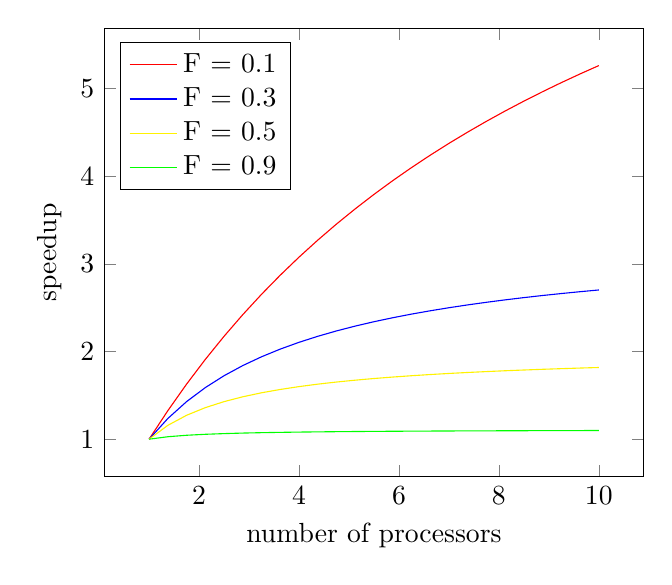
\begin{tikzpicture}
  \begin{axis}[
    xlabel = number of processors,
    ylabel =speedup,
    legend pos = north west,]
 \addplot[domain=1:10, color=red] {1/(0.1+(1-0.1)/x)}; 
 \addlegendentry{F = 0.1}
 \addplot[domain=1:10, color=blue] {1/(0.3+(1-0.3)/x)};
 \addlegendentry{F = 0.3}
 \addplot[domain=1:10, color=yellow] {1/(0.5+(1-0.5)/x)};
 \addlegendentry{F = 0.5}
 \addplot[domain=1:10, color=green] {1/(0.9+(1-0.9)/x)};
 \addlegendentry{F = 0.9}
 \end{axis}
\end{tikzpicture}
\label{fig:plot_cpu}

The graph shows how the performance gained by adding processors depends on the type of the computation. A computation that cannot be parallelized much (high value of F) will have a low performance increase with more processors. 

\subsection{Load balancing}

Let's consider a single CPU with multiple cores. To achieve the best possible performance, the workload should be spread evenly between the cores, and there shouldn't be any core that does significantly less work than another. It is up to the scheduler to keep the load of each core balanced.

How is the load measured? The first option is to use the weights of the task. The load of a core would be the sum of the weights of its tasks, but this approach doesn't work very well. Suppose that we have 4 tasks with the same priority, 2 are CPU intensive and 2 spend most of their time sleeping, and we want to balance the load between 2 processors. If we use only the weights of the tasks to balance, both the CPU intensive tasks could get assigned to one core, making it always busy, while the other core would be almost always idle as both of his tasks spend most of their time waiting. This approach doesn't take into consideration the nature of the tasks (CPU bound vs I/O bound). To effectively measure the load, we need to keep track of the amount of time that a task spends sleeping. Hence, the load of a task becomes a combination of its weight and its average CPU utilization, and the load of the a core is the sum of the loads of its tasks. Since the CPU utilization of a task can vary, its load is constantly updated.

\subsubsection{Migrating tasks}
The scheduler periodically checks that the load of all the CPUs is balanced. In case it is not, the scheduler tries to migrate the tasks from one CPU to another: this operation is called \textit{task migration}. The migration of a task could be expensive and, in some cases, it could be more efficient to not move the task at all. The memory access design of the CPU plays an important role and can change radically how expensive it is to migrate tasks. In a \textit{uniform memory access} (UMA) architecture there is one memory, and the cost of accessing it is the same for all the cores. In this case the tasks can be migrated between cores without any constraints, but having a single memory is not efficient since two cores cannot access the memory at the same time. Modern processors solve this problem by giving each core its own memory, but this creates a more complex structure. In \textit{non-uniform memory access} (NUMA) the cost of accessing the memory is no longer the same for all the cores, but depends on where the desired data is located. Specifically, memory can be local or foreign relatively to a core, and the migration cost changes drastically between the two. This means that sometimes it is more efficient to keep a task on the same core, even if the cores are not balanced. 

\begin{figure}[ht]
\includegraphics[width=\textwidth]{images/numa.png}
\caption{Local and foreign memory in a NUMA architecture}
\label{img:numa}
\end{figure}
The same system could use a mix of the two structures: the cores could be divided in groups with their own memory. Accessing the memory of another group is more expensive, but inside a group all the cores can access the memory at same cost. Inside a group tasks can be migrated more frequently, while migration between groups should be less frequent. To efficiently use this structure the system gives the possibility of defining different migration policies.

\paragraph{Domains} %mpi
The structure of the system is described by two entities: scheduling domains and CPU groups. A scheduling domain is a set of CPUs, and a CPU group is a partition of the CPUs of a domain. A CPU inside a domain cannot belong to two groups of the same domain and every CPU has to be part of a group. The scheduler does not balance the load between single CPUs, instead it tries to balance the loads among the CPU groups of a domain.

Let's take as an example a system with 2 pairs of processors. A pair shares the same memory and its processors can exchange tasks without cost. On the other hand, moving tasks between pairs is more expensive. This could be a real scenario, where a pair represents a single physical processor with inside two hyperthreaded CPUs. Each pair is represented by a domain, which contains two CPU groups, one for each processor. The groups contains only one CPU in this case. Inside this domain balancing can happen very often since it can be done without additional cost, and it is triggered by small differences in load between the groups of the domain.

To allow the tasks to be migrated from one domain to another, there is also an higher level domain that includes all the CPUs. It is partitioned in two CPU groups, one for each pair. The two groups are kept balanced, but the scheduler does not try to balance the load inside a group. This domain tries to balance the load much less often and it is more tolerant to imbalances in the load. There could also be other layers of domains: for example, in a NUMA system there could be another domain representing a NUMA node, with a different migration policy. By using this domain structure, the scheduler can take in consideration the organization of the system when balancing the CPUs, allowing for more efficient choices.
\chapter{Implementation of the Linux scheduler}
\label{chap:implementation}

\section{Structs and their role}

\paragraph{task\_struct}
As mentioned in chapter \ref{ch:introduction}, each task in the system is represented \newline by a \verb|task_struct|, which contains all the information about it. Here we list some of the fields used by the scheduler, and then cover them in detail.
\begin{itemize}
    \item \verb|thread_info|. This struct is architecture dependant and can contain various fields. The most important for the scheduler is the \verb|flags| field. These flags are used to keep track of requests or signals from and for the task. \verb|TIF_SIGPENDING| means that the process has pending signals, \verb|TIF_MEMDIE| means that the process is being killed to reclaim memory. In particulare, there are two flags that are crucial for the scheduler: \verb|TIF_NEED_RESCHED| and \verb|TIF_POLLING_NRFLAG|. The first indicates that scheduling must be performed, and the second that the idle process is polling the \verb|TIF_NEED_RESCHED| flag.
    %from cesati's book
    \item \verb|state|. A long that represents the state of the task: -1 unrunnable, 0 runnable, $>0$ stopped. 
    \item \verb|on_rq|. Indicates if the process is on the runqueue.
    \item \verb|static_prio| and \verb|normal_prio|. The first is the priority used for real-time scheduling policies. If the task is scheduled under one of the normal scheduling policies \verb|static_prio| is set to zero and \verb|normal_prio| is used. This number is an internal representation used in the kernel, different from the priority value shown in user space.
    \item \verb|sched_entity|. This struct contains all the other information needed by the scheduler.
    \item Pointer to \verb|sched_class|. The scheduling class discussed in chapter \ref{ch:sched}. Contains a circular list of all scheduling classes.
    \item Pointer to \verb|mm_struct|. This struct represents the slice of virtual memory used by the process. Here, ``\verb|mm|'' stands for \textit{memory management}.
\end{itemize}

\paragraph{thread\_info}
\label{sec:thread_info}
This structure is very small and contains only basic information useful for scheduling, and each process has its own \verb|thread_info|. In figure \ref{img:stack} from chapter \ref{ch:introduction} it is shown that this struct is located at the bottom of kernel stacks. The small size of this struct is due to the fact that it has to fit in the small kernel stacks while not occupying too much space. Today, the implementation of \verb|thread_info| has changed: it is now embedded directly in \verb|task_struct|. 

\begin{code}
struct task_struct {
#ifdef CONFIG_THREAD_INFO_IN_TASK
	/*
	 * For reasons of header soup (see current_thread_info()), this
	 * must be the first element of task_struct.
	 */
	struct thread_info  thread_info;
#endif
// ...
\end{code}
With the previous implementation, \verb|thread_info| and \verb|task_struct| referenced each other through pointers. As shown in this code, if \verb|CONFIG_THREAD_INFO_IN_TASK| is defined, the field is not a pointer. With this new implementation, \verb|thread_info| is not located in the kernel stack. In order to access it, a pointer to the current task's \verb|thread_info| is saved, and its \verb|task_struct| can be accessed with the ``\verb|container_of()| trick'' discussed in chapter \ref{ch:introduction}. 

The implementation of this struct is very architecture dependent. This one is specific to x86:
\begin{code}
struct thread_info {
	unsigned long   flags;  /* low level flags */
	u32 status;             /* thread synchronous flags */
};
\end{code}
The flags field is crucial, because it is here that the \verb|TIF_NEED_RESCHED| flag is set, allowing the scheduler to be invoked. In practice, there are pieces of code that are executed each time a task enters/exits kernel space. In particular, when returning to user space, each task will execute the \textit{userspace return path}, defined in assembly in \verb|./arch/x86/entry_64.S|. This code checks the \verb|TIF_NEED_RESCHED| flag, and if set will call the \verb|schedule()| routine. We said earlier that the scheduler code is executed by any user process that was going to return to user space: this is the exact point in the kernel where it happens.

\paragraph{sched\_entity}
The \verb|sched_entity| struct represent a \textit{schedulable entity}. From the scheduler's perspective, there is no difference between a process, a thread or even a whole group of processes: they are all just schedulable entities represented by this struct, and scheduler is oblivious to their real nature. Because of this, the scheduler works only with schedulable entities and not \verb|task_struct|s. For example, runqueues contain schedulable entities. 

A \verb|sched_entity| may be organized in a hierarchy of entities, this is done to allow group scheduling and it is optional. Suppose that there are more users using a system and we want to share the CPU equally between them, but they have different processes running. With normal CFS, each task is present in the runqueue and it is scheduled independently. By organizing the entities in hierarchies, we can group together the tasks and schedule them as a single schedulable entity. In the previous example we would have only two entities on the runqueue, one for each user, and a corresponding runqueue containing all the task of that user. The scheduler decides which of the two entities to schedule, as if there were only two tasks running, and then repeats the process for the sub-queue. As stated earlier, a \verb|sched_entity| does not always correspond to a process; only the leafs of this structure correspond to a task. 

The most important fields that compose \verb|sched_entity| are:
\begin{itemize}
    \item \verb|load_weight|. It contains the weight of the entity. The role of the weight is discussed in chapter \ref{ch:sched}.
    \item \verb|struct rb_node run_node|. Represents a node inside a red-black tree. The next section shows that the runqueue is organized as a red-black tree. This field is embedded in this struct because the implementation is similar to lists.
    \item \verb|on_rq|. Indicates if the entity is on the runqueue.
    \item \verb|exec_start|. The time at which the task started its execution on the CPU. %resetted each time (calc_delta_fair)
    \item \verb|sum_exec_runtime|. The total time that the task has actually spent running on the CPU before being weighted.
    \item \verb|vruntime|. The weighted total time that the task has spent running.
    \item \verb|struct sched_entity *parent|. The parent node in the hierarchy.
    \item \verb|struct cfs_rq *cfs_rq|. The runqueue on which this entity is queued.
    \item \verb|struct cfs_rq *my_q|. If this is a group, this is the sub-runqueue of this group. The children of this entity are queued here.
\end{itemize}
These fields are specific to CFS, where the runqueue is a red-black tree (\verb|rb_node| and \verb|cfs_rq|), and the timeslice is based on virtual runtime (\verb|exec_start| and \verb|sum_exec_runtime| are used to calculate vruntime). The other scheduling class have their own entity, such as \verb|sched_rt_entity| and \verb|sched_dl_entity|, defining its specific fields. \verb|sched_entity| is not called \verb|sched_fair_entity| supposedly because the fair class is the default. 

\paragraph{sched\_class}
\label{sec:sched_class}
This structure contains function pointers to the scheduler routines, specific to the scheduling class. Each class has routines that do the same thing, but with different implementations.

\begin{code}
struct sched_class {
	const struct sched_class *next; //Circular list of all classes

	void (*enqueue_task) (struct rq *rq, struct task_struct *p, int flags);
	void (*dequeue_task) (struct rq *rq, struct task_struct *p, int flags);
	void (*yield_task)   (struct rq *rq);
	bool (*yield_to_task)(struct rq *rq, struct task_struct *p, bool preempt);
	void (*check_preempt_curr)(struct rq *rq, struct task_struct *p, int flags);

	/*
	 * It is the responsibility of the pick_next_task() method that will
	 * return the next task to call put_prev_task() on the @prev task or
	 * something equivalent.
	 *
	 * May return RETRY_TASK when it finds a higher prio class has 
	 * runnable tasks.
	 */
	struct task_struct * (*pick_next_task)(struct rq *rq,
					       struct task_struct *prev,
					       struct rq_flags *rf);
    // ...
    void (*task_tick)(struct rq *rq, struct task_struct *p, int queued);
    void (*update_curr)(struct rq *rq);
    // ...
}
\end{code}
When scheduling, the class list is visited, starting from the higher priority class: if there is no process to schedule the next class is visited. This keeps going until something to schedule is found, then the correct function pointers are used to carry out the scheduler's jobs. In \verb|fair.c| we can find the declaration of the \verb|sched_class| specific for the fair class:
\begin{code}
/*
 * All the scheduling class methods:
 */
const struct sched_class fair_sched_class = {
	.next			= &idle_sched_class,
	.enqueue_task		= enqueue_task_fair,
	.dequeue_task		= dequeue_task_fair,
	.yield_task		= yield_task_fair,
	.yield_to_task		= yield_to_task_fair,

	.check_preempt_curr	= check_preempt_wakeup,

	.pick_next_task		= pick_next_task_fair,
	.put_prev_task		= put_prev_task_fair,

#ifdef CONFIG_SMP
	.select_task_rq		= select_task_rq_fair,
	.migrate_task_rq	= migrate_task_rq_fair,

	.rq_online		= rq_online_fair,
	.rq_offline		= rq_offline_fair,

	.task_dead		= task_dead_fair,
	.set_cpus_allowed	= set_cpus_allowed_common,
#endif

	.set_curr_task          = set_curr_task_fair,
	.task_tick		= task_tick_fair,
	.task_fork		= task_fork_fair,

	.prio_changed		= prio_changed_fair,
	.switched_from		= switched_from_fair,
	.switched_to		= switched_to_fair,

	.get_rr_interval	= get_rr_interval_fair,

	.update_curr		= update_curr_fair,

#ifdef CONFIG_FAIR_GROUP_SCHED
	.task_change_group	= task_change_group_fair,
#endif
};
\end{code}
This structure is a good reference to understand the code because it essentially lists all the main CFS scheduler routines, which are covered in the next section. 

% https://www.tldp.org/LDP/tlk/kernel/processes.html
\paragraph{mm\_struct} 
This data structure abstracts the virtual memory of a process. It contains information about the executable image of the process, a pointer to the process's page tables, and a mapping to the virtual memory areas. Figure \ref{img:mm} shows the fundamental fields of the struct.

\begin{figure}[ht]
\includegraphics[width=\textwidth]{images/mm.jpg}
\caption{The structures used for virtual memory \url{https://www.tldp.org/LDP/tlk/kernel/processes.html}}
\label{img:mm}
\end{figure}
\verb|mmap| contains a list of virtual memory areas, which can contain the executable code, data, or code from shared libraries.
This list is actually organized in a binary tree, ordered by memory address, for faster access. These areas are allocated by the process as it runs, for example when it loads code of a shared library. Because it is virtual memory, each process has the illusion that it has the whole memory for itself, and that each time that it allocates memory it gets physically allocated. Such an approach would waste memory: what if the shared library is already loaded in RAM and used by other processes?

For this reason, Linux uses \textit{on-demand paging}. When a process allocates virtual memory, Linux does not actually reserve physical memory for the process. Instead, it describes the virtual memory by creating a new \verb|vm_area_struct| data structure. This is linked into the process's list of virtual memory. When the process attempts to write to a virtual address within that new virtual memory region then the system will page fault. Linux looks to see if the virtual address referenced is in the current process's virtual address space. If it is, Linux creates the appropriate \textit{page table entries} (PTEs) and allocates a physical page of memory for this process. The code or data may need to be brought into that physical page from the filesystem or from the swap disk. The process can then be restarted at the instruction that caused the page fault and, this time as the memory physically exists, it may continue.\cite{tlk}

\verb|mm_struct| has also a role in scheduling, because the \verb|mm|s of the two processes are switched upon context switch. The field \verb|mm| can also be set to \verb|NULL|: in this case the task is a kernel thread, free to use all the kernel space. This operation can be seen in the \verb|context_switch()| routine in Section \ref{sec:context_switch}.

\paragraph{procfs}
The information contained in these structures can be accessed from outside the kernel with specific tools (covered in detail in Chapter \ref{chap:ftrace}). One approach to accomplish this it to use \verb|procfs|. In short, \verb|procfs| is a special filesystem that contains all the kernel information about processes, making it easy to access it from user space. For example, it is possible to gather scheduling information about process with pid 1196 by executing \verb|cat /proc/1196/schedstat|. This gives the following human-readable output:

\begin{verbatim}
tilda (1196, #threads: 3)
-------------------------------------------------------------------
se.exec_start                                :      26964101.112552
se.vruntime                                  :       2272975.687429
se.sum_exec_runtime                          :         10181.684621
se.nr_migrations                             :                11160
nr_switches                                  :                40529
nr_voluntary_switches                        :                40104
nr_involuntary_switches                      :                  425
se.load.weight                               :              1048576
se.avg.load_sum                              :              2453334
se.avg.util_sum                              :              2417183
se.avg.load_avg                              :                   45
se.avg.util_avg                              :                   45
se.avg.last_update_time                      :       26964101112552
policy                                       :                    0
prio                                         :                  120
clock-delta                                  :                   50
mm->numa_scan_seq                            :                    0
numa_pages_migrated                          :                    0
numa_preferred_nid                           :                   -1
total_numa_faults                            :                    0
current_node=0, numa_group_id=0
numa_faults node=0 task_private=0 task_shared=0 
group_private=0 group_shared=0
\end{verbatim}
Here, ``\verb|se|'' is the name of the field of type \verb|sched_entity| in \verb|task_struct|.

\paragraph{Red-black tree}
\label{sec:rb-tree}
The runnable tasks are stored inside a red-black tree, which allows more efficiency. A red-black tree is a type of self-balancing binary search tree: this means that the insertion and deletion operations will keep the height of the tree as small as possible. This characteristic is important because the cost of the most common functions (search, insertion and deletion) is proportional to the height of the tree.
As stated before, the task to run next is the one with the smallest vruntime. In a red-black tree, this corresponds to the task in the leftmost node. When picking the next task the tree is not traversed, instead, the leftmost node is cached in a dedicated variable in order to retrieve it faster.

\section{Time keeping}
\label{sec:timekeeping}
The kernel must keep track of time. The scheduler, for example, needs to know for how long a task has been running in order to know when to preempt it. There are many other functions that are time-driven, so it's important to understand how the system keeps track of the time.

To do this, the kernel requires an hardware timer. This timer can be implemented in different ways and there can be more timers in a system, but the general idea is the same: the timer sends an interrupt at a fixed frequency known by the kernel. This way, it's possible to get the time between two timer interrupts and perform periodic actions such as updating the system uptime. The period between two interrupts is a unit of measure called \textit{tick}, while the frequency is called \textit{tick rate}; this value is internally defined as the constant \texttt{HZ}. If the value of \texttt{HZ} is 100, there are 100 ticks per second, or one tick each 10 milliseconds.

\subsubsection{Choice of the tick rate}
Changing the frequency of the timer interrupt can have a large impact on the behavior of the system, so there are pros and cons to larger or smaller values of \texttt{HZ}.

%pros of larger HZ
A larger \texttt{HZ} means that the timer interrupt has a finer granularity: this means that all the timed events also have a higher resolution, which allows to improve their accuracy. As an example, let's consider process preemption: with an higher tick rate we can improve the accuracy and reduce the scheduling latency. Suppose that a process has 2 milliseconds left of its timeslice and the timer interrupt has just occurred. With an \texttt{HZ} of 100 the next interrupt will occur in 10 milliseconds, giving the process 8 extra milliseconds. This means that another task has to wait for more time in the runqueue, and this can be an issue for time-sensitive tasks. With a larger \texttt{HZ}, for example 1000, in the worst case scenario the latency is only 1 millisecond.

%cons of larger HZ
There is also a drawback to increasing the tick rate: the interrupt handler gets executed more often, and this results in less processor time for the tasks. The actual impact of the increased overhead is debatable and depends heavily on the speed of the processor.

%different values of HZ
The value of \texttt{HZ} depends on hardware and on the kernel configuration. On i386 \texttt{HZ} had a value of 100, with Linux version 2.6 the value was raised to 1000 and later was made a configurable parameter, with a default of 250. There were also introduced other, more accurate and \texttt{HZ}-independent, timers called \textit{high resolution timers} (HRT), making a high \texttt{HZ} less necessary. It is also possible to configure the kernel as \textit{tickless} (\verb|NO_HZ|): this means that the interrupt is no longer at fixed intervals, but it's dynamically scheduled as needed, which is helpful for power saving.

\subsubsection{Jiffies}
%What is jiffies
``\textit{Jiffies}'' is the number of ticks that have occurred since the system started. Every time that the interrupt handler is executed, the value of jiffies is increased by one. This means that with the value of \texttt{HZ}, and the value of jiffies, we can easily convert from seconds to jiffies by doing \verb|seconds * HZ| and from jiffies to seconds with \verb|jiffies / HZ|.
\begin{code}
// ./kernel/sched/sched.h
/*
 * Helpers for converting nanosecond timing to jiffy resolution
 */
#define NS_TO_JIFFIES(TIME) ((unsigned long)(TIME) / (NSEC_PER_SEC / HZ))
\end{code}

\paragraph{sched\_clock()}
\label{sched_clock}
An important function is \verb|sched_clock()|: it returns the system's uptime in nanoseconds. An architecture may provide an implementation, but if it is not provided, the system will use the jiffies counter to calculate the system's uptime.

The scheduler uses this function to determine the absolute, non-weighted, time that the current task has been running (\verb|se->runtime|). If the system uses the jiffies counter to determine this value, the maximum resolution of \verb|sched_clock()| depends on \texttt{HZ}. In this case the choice of \texttt{HZ} becomes more relevant.
The following is the default implementation of \verb|sched_clock()| when using only jiffies:
\begin{code}
unsigned long long __weak sched_clock(void)
{
	return (unsigned long long)(jiffies - INITIAL_JIFFIES)
					* (NSEC_PER_SEC / HZ);
}
\end{code}

\subsubsection{Timer interrupt handler}

The timer interrupt handler invokes other functions, some of which are architecture dependent. The other, architecture independent, timer functions are executed by \verb|tick_periodic()|, which is called by the handler.

\begin{code}
// ./kernel/time/tick-common.c
static void tick_periodic(int cpu)
{
	if (tick_do_timer_cpu == cpu) {
		write_seqlock(&jiffies_lock);

		/* Keep track of the next tick event */
		tick_next_period = ktime_add(tick_next_period, tick_period);

		do_timer(1);
		write_sequnlock(&jiffies_lock);
		update_wall_time();
	}

	update_process_times(user_mode(get_irq_regs()));
	profile_tick(CPU_PROFILING);
}
\end{code}
The two most important functions here are \verb|do_timer()| and \verb|update_process_times()|. The first one increments the value of jiffies and updates the load statistics for the system. The second updates various statistics and the runtime of the current task: if the task has finished its timeslice, it will prompt a reschedule. %TIF_NEED_RESCHED?

\begin{code}
// ./kernel/time/tick-common.c
/*
 * Must hold jiffies_lock
 */
void do_timer(unsigned long ticks)
{
	jiffies_64 += ticks;
	calc_global_load(ticks);
}
\end{code}

\subsubsection{update\_process\_times()}
This function updates the time that the current process has been running. The procedure changes if the process was running in user mode or in kernel mode. Remember that \verb|task_struct| has two different fields \verb|utime| and \verb|stime| to keep track of time spent in user space and in kernel space respectively. This function also invokes the \verb|scheduler_tick| function, which is the entry point that calls all the scheduler routines.

\begin{code}
// ./kernel/time/timer.c
/*
 * Called from the timer interrupt handler to charge one tick to the current
 * process.  user_tick is 1 if the tick is user time, 0 for system.
 */
void update_process_times(int user_tick)
{
	struct task_struct *p = current;

	/* Note: this timer irq context must be accounted for as well. */
	account_process_tick(p, user_tick);
	run_local_timers();
	rcu_check_callbacks(user_tick);
#ifdef CONFIG_IRQ_WORK
	if (in_irq())
		irq_work_tick();
#endif
	scheduler_tick();
	if (IS_ENABLED(CONFIG_POSIX_TIMERS))
		run_posix_cpu_timers(p);
}
\end{code}

\section{Scheduler routines}
There are essentially two ways of prompting a reschedule:
\begin{itemize}
    \item When the timeslice of the current process expires. When this occurs, the \verb|TIF_NEED_RESCHED|
    flag in the \verb|thread_info| structure of the current process is set, so the scheduler is
    invoked when the timer interrupt handler terminates.\cite{cesati} This rescheduling possibility is checked periodically, at each system tick.
    \item When a task is added to the runqueue. When it happens, the kernel checks whether its dynamic priority is greater than the priority of the currently running process. If it is, the wakeup sets \verb|TIF_NEED_RESCHED|, and the scheduler will eventually be invoked to select another process to run
    (usually the process that just became runnable).\cite{cesati} This rescheduling possibility is checked every time that a task is created or woken up.
\end{itemize}
The internal workings of these two procedures is illustrated, in order, in the two upcoming sections. There are other times in which a reschedule is prompted: indeed, \verb|schedule()| could be called like any other function, but this is done rarely in practice.

\subsection{Periodic reschedule}
\label{sec:periodic_reschedule}
We will now analyze in detail how scheduling works and the most important functions involved. In the last section, we saw how the system can perform periodic functions in order to measure time. From the entry point \verb|scheduler_tick()|, the subsequent calls can be traced with \verb|ftrace|: a function/event tracer embedded in the kernel.

The following script can trace function calls of any input kernel function. Function tracing with \verb|ftrace| is explained in detail in Chapter \ref{chap:ftrace}. For now, it is enough to know that this script simply sets \verb|ftrace| parameters before starting the trace. 
\begin{codebash}
#!/bin/bash
echo function_graph > /sys/kernel/debug/tracing/current_tracer
# removing noise to see just the actual function trace
# trace on cpu0 only (actually disables tracing on other cpus)
echo 1 > /sys/kernel/debug/tracing/tracing_cpumask 
# show comments on all exit points
echo funcgraph-tail > /sys/kernel/debug/tracing/trace_options 
# function to trace
echo $* > /sys/kernel/debug/tracing/set_graph_function
# clear previous trace
echo > /sys/kernel/debug/tracing/trace
sleep 3
cat /sys/kernel/debug/tracing/trace
\end{codebash}
%show trace starting from the timer interrupt, using function_graph tracer
With ``\verb|scheduler_tick|'' as input, this is a small piece of the output trace. Next, it is shown what's inside these functions.
\begin{Verbatim}
0)               |  scheduler_tick() {
0)   0.238 us    |    _raw_spin_lock();
0)   0.207 us    |    update_rq_clock.part.84();
0)               |    task_tick_fair() {
0)               |      update_curr() {
0)   0.167 us    |        update_min_vruntime();
0)   0.305 us    |        cpuacct_charge();
0)   3.652 us    |      } /* update_curr */
0)   0.219 us    |      __compute_runnable_contrib();
0)   0.159 us    |      __compute_runnable_contrib();
0)   0.114 us    |      intel_pstate_update_util();
0)   0.263 us    |      update_cfs_shares();
0)   0.178 us    |      hrtimer_active();
0) + 15.135 us   |    } /* task_tick_fair */
0)               |    cpu_load_update_active() {
0)   0.163 us    |      tick_nohz_tick_stopped();
0)               |      cpu_load_update() {
0)   0.178 us    |        sched_avg_update();
0)   1.927 us    |      } /* cpu_load_update */
0)   5.132 us    |    } /* cpu_load_update_active */
0)   0.148 us    |    calc_global_load_tick();
0)               |    trigger_load_balance() {
0)   0.400 us    |      idle_cpu();
0)   2.760 us    |    } /* trigger_load_balance */
0) + 33.332 us   |  } /* scheduler_tick */
\end{Verbatim}
In the following pieces of code, ``\verb|likely()|'' and ``\verb|unlikely()|'' are macros for \verb|gcc|'s built in branch prediction.
\begin{code}
// ./include/linux/compiler.h
#define likely(x)       __builtin_expect(!!(x), 1)
#define unlikely(x)     __builtin_expect(!!(x), 0)
\end{code}
These two macros are used in conditions. They indicate, respectively, that the condition is expected to be true or false. \verb|gcc| will then produce the correct assembly at compile time. If the guess is correct, less CPU cycles are used to choose the branch, but if it's not, the cycles are doubled. The double inversion (\verb|!!|) is to make sure the parameter is binary.

\subsubsection{scheduler\_tick}
As stated earlier, this function is called by the interrupt handler at every system tick.

\begin{code}
// ./kernel/sched/core.c
void scheduler_tick(void)
{
	int cpu = smp_processor_id();
	struct rq *rq = cpu_rq(cpu);
	struct task_struct *curr = rq->curr;
	struct rq_flags rf;

	sched_clock_tick();

	rq_lock(rq, &rf);

	update_rq_clock(rq);
	curr->sched_class->task_tick(rq, curr, 0);
	cpu_load_update_active(rq);
	calc_global_load_tick(rq);
	psi_task_tick(rq);

	rq_unlock(rq, &rf);

	perf_event_task_tick();

#ifdef CONFIG_SMP
	rq->idle_balance = idle_cpu(cpu);
	trigger_load_balance(rq);
#endif
}
\end{code}
The first important function here is \verb|sched_clock_tick()|. This function updates the per-CPU \verb|sched_clock_data| struct. To update this time, it uses the \verb|sched_clock()| function discussed earlier.

\verb|update_rq_clock()| updates the \verb|clock_task| field inside the runqueue of the current CPU (\verb|cpu_rq(cpu)|). This is used later by \verb|update_curr()|, a function that updates the \verb|task_struct| of the currently running process (stats, vruntime, runtime\dots).

Then, on line 14, \verb|task_tick()| is invoked for the current task to update its statistics. This action depends on the scheduling class that the current process is using. As shown in Section \ref{sec:sched_class}, \verb|sched_class| contains hooks to the correct functions for each scheduling class. Suppose that the current task has the fair class, then \verb|task_tick_fair()| would be executed on this line.

\subsubsection{task\_tick\_fair}

The runtime statistics for the current process are stored in the \verb|sched_entity| associated with it. The scheduler updates its parameters and then checks if the current task is to be rescheduled. 

\begin{code}
// ./kernel/sched/fair.c
static void task_tick_fair(struct rq *rq, struct task_struct *curr, int queued)
{
	struct cfs_rq *cfs_rq;
	struct sched_entity *se = &curr->se;

	for_each_sched_entity(se) {
		cfs_rq = cfs_rq_of(se);
		entity_tick(cfs_rq, se, queued);
	}

	if (static_branch_unlikely(&sched_numa_balancing))
		task_tick_numa(rq, curr);

	update_misfit_status(curr, rq);
}
\end{code}
This function fetches the \verb|sched_entity| of the current process. This is going to be a leaf of the hierarchy, and if the task isn't part of a group, it is also the root. Remember that the \verb|sched_entity| struct points to two runqueues: \verb|cfs_rq| and \verb|my_q|. The first is the runqueue on which the entity is scheduled, the second is the runqueue that belongs to that group. When the entity is a leaf, the second field is empty. 

For each entity in the hierarchy starting from the leaf, the function calls:
\begin{itemize}
    \item \verb|cfs_rq_of(se)|. This returns the runqueue on which the entity is scheduled. If the system is configured without group scheduling there is only one runqueue.
    
    \item \verb|entity_tick(cfs_rq, se, queued)|. This updates the statistics of that entity, then checks if it has finished its time and if another entity deserves to run. This means that:
    \begin{enumerate}
        \item If a process inside a group still deserves more time
        \item but the entire group has finished its time
        \item and another group deserves the CPU
    \end{enumerate}
    Then the task is preempted anyway. \verb|entity_tick()| also updates the load statistics used to balance the load between CPUs.
\end{itemize}

\subsubsection{entity\_tick}
\begin{code}
// ./kernel/sched/fair.c
static void
entity_tick(struct cfs_rq *cfs_rq, struct sched_entity *curr, int queued)
{
	/*
	 * Update run-time statistics of the 'current'.
	 */
	update_curr(cfs_rq);

	/*
	 * Ensure that runnable average is periodically updated.
	 */
	update_load_avg(cfs_rq, curr, UPDATE_TG);
	update_cfs_group(curr);

#ifdef CONFIG_SCHED_HRTICK
	/*
	 * queued ticks are scheduled to match the slice, so don't bother
	 * validating it and just reschedule.
	 */
	if (queued) {
		resched_curr(rq_of(cfs_rq));
		return;
	}
	/*
	 * don't let the period tick interfere with the hrtick preemption
	 */
	if (!sched_feat(DOUBLE_TICK) &&
			hrtimer_active(&rq_of(cfs_rq)->hrtick_timer))
		return;
#endif

	if (cfs_rq->nr_running > 1)
		check_preempt_tick(cfs_rq, curr);
}
\end{code}
\subsubsection{update\_curr}
\label{sec:update_curr}

The first part of \verb|entity_tick()|'s job, updating the runtime statistics, is done by \verb|update_curr()|. This function takes as argument only the runqueue on which the current task is running. From the runqueue, it gets the \verb|sched_entity| of the current task. It also gets the current time from the runqueue's clock, previously updated through \verb|update_rq_clock()|.

\label{trace:sched_stat_runtime}
\begin{code}
// ./kernel/sched/fair.c
static void update_curr(struct cfs_rq *cfs_rq)
{
	struct sched_entity *curr = cfs_rq->curr;
	u64 now = rq_clock_task(rq_of(cfs_rq));
	u64 delta_exec;

	if (unlikely(!curr))
		return;

	delta_exec = now - curr->exec_start;
	if (unlikely((s64)delta_exec <= 0))
		return;

	curr->exec_start = now;

	schedstat_set(curr->statistics.exec_max,
		      max(delta_exec, curr->statistics.exec_max));

	curr->sum_exec_runtime += delta_exec;
	schedstat_add(cfs_rq->exec_clock, delta_exec);

	curr->vruntime += calc_delta_fair(delta_exec, curr);
	update_min_vruntime(cfs_rq);

	if (entity_is_task(curr)) {
		struct task_struct *curtask = task_of(curr);

		trace_sched_stat_runtime(curtask, delta_exec, curr->vruntime);
		cgroup_account_cputime(curtask, delta_exec);
		account_group_exec_runtime(curtask, delta_exec);
	}

	account_cfs_rq_runtime(cfs_rq, delta_exec);
}
\end{code}
\verb|curr->exec_start| is the time at which the entity was selected by the scheduler to be executed. %pick_next_entity()->set_next_entity()->update_stats_curr_start()
We can calculate \verb|delta_exec|, the amount of time that the task has spent running, simply by subtracting \verb|exec_start| from the current time. \verb|exec_start| is then reset to the current time. \verb|delta_exec| is used to update the total \textbf{actual} runtime of the entity (\verb|sum_exec_runtime|). Other statistics are also updated, such as the longest execution so far (\verb|statistics.exec_max|).

The virtual runtime is the total runtime weighted. The weighted delta is calculated on line 22 by \verb|calc_delta_fair()|, and the virtual runtime is updated.
If the newly calculated vruntime is also the smallest in the runqueue, the field \verb|cfs_rq->min_vruntime()| is updated.
\verb|update_curr()| also triggers the trace event \verb|sched_stat_runtime|: this event signals when a process' virtual runtime is updated.

It is also possible that a group of tasks has a limit on the amount of CPU it can use. The function \verb|account_cfs_rq_runtime| is specific for groups. It updates \verb|cfs_rq->remaining_runtime|, where \verb|cfs_rq| is, again, the runqueue of the current group; then it triggers a reschedule if the remaining time reaches zero.

\subsubsection{calc\_delta\_fair and \_\_calc\_delta}
This function and its subfunction are a mere application of equation \ref{eq:vruntime}. Like the formula, this function weights the delta. \verb|__calc_delta| is where it's applied: it also takes the same parameters as the equation. 
\begin{code}
// ./kernel/sched/fair.c
/*
 * delta /= w
 */
static inline u64 calc_delta_fair(u64 delta, struct sched_entity *se)
{
	if (unlikely(se->load.weight != NICE_0_LOAD))
		delta = __calc_delta(delta, NICE_0_LOAD, &se->load);

	return delta;
}
\end{code}
\subsubsection{check\_preempt\_tick}

\verb|check_preempt_tick()| is called at the end of \verb|entity_tick()|, after all the fields of the current process have been updated with \verb|update_curr()|. Its job is to check if the current task has to be preempted. 
\begin{code}
// ./kernel/sched/fair.c
/*
 * Preempt the current task with a newly woken task if needed:
 */
static void
check_preempt_tick(struct cfs_rq *cfs_rq, struct sched_entity *curr)
{
	unsigned long ideal_runtime, delta_exec;
	struct sched_entity *se;
	s64 delta;

	ideal_runtime = sched_slice(cfs_rq, curr);
	delta_exec = curr->sum_exec_runtime - curr->prev_sum_exec_runtime;
	if (delta_exec > ideal_runtime) {
		resched_curr(rq_of(cfs_rq));
		/*
		 * The current task ran long enough, ensure it doesn't get
		 * re-elected due to buddy favours.
		 */
		clear_buddies(cfs_rq, curr);
		return;
	}

	/*
	 * Ensure that a task that missed wakeup preemption by a
	 * narrow margin doesn't have to wait for a full slice.
	 * This also mitigates buddy induced latencies under load.
	 */
	if (delta_exec < sysctl_sched_min_granularity)
		return;

	se = __pick_first_entity(cfs_rq);
	delta = curr->vruntime - se->vruntime;

	if (delta < 0)
		return;

	if (delta > ideal_runtime)
		resched_curr(rq_of(cfs_rq));
}
\end{code}
The first step is calculating \verb|ideal_runtime|. As the name suggests, this is the timeslice assigned to the task: remember that CFS's timeslice always varies dynamically.

If the task has run for more than the ideal runtime, the function \verb|resched_curr()| is called and it will cause the preemption of the task. The other way this function can trigger a reschedule, is if the difference between the virtual runtime of the current task and the smallest virtual runtime in the runqueue is bigger than the ideal runtime.

\paragraph{sched\_slice}
\begin{code}
/*
 * We calculate the wall-time slice from the period by taking a part
 * proportional to the weight.
 *
 * s = p*P[w/rw]
 */
static u64 sched_slice(struct cfs_rq *cfs_rq, struct sched_entity *se)
{
	u64 slice = __sched_period(cfs_rq->nr_running + !se->on_rq);

	for_each_sched_entity(se) {
		struct load_weight *load;
		struct load_weight lw;

		cfs_rq = cfs_rq_of(se);
		load = &cfs_rq->load;

		if (unlikely(!se->on_rq)) {
			lw = cfs_rq->load;

			update_load_add(&lw, se->load.weight);
			load = &lw;
		}
		slice = __calc_delta(slice, se->load.weight, load);
	}
	return slice;
}
\end{code}
\verb|sched_slice()| first calculates $target\_latency$ of equation \ref{eq:assigned_time}---also known as the \textit{scheduler period}. Remember that this value is defined as a period of time in which each task runs once, for at least \verb|sysctl_sched_min_granularity| nanoseconds. It is calculated through \verb|__sched_period()|.\label{sec:sched_period}
Here, two important scheduler tunables are used:
\begin{itemize}
    \item \verb|sysctl_sched_min_granularity| -- the minimum time a task is be allowed to run on a CPU before being preempted.
    \item \verb|sysctl_sched_latency| -- the default scheduler period.
\end{itemize}
\begin{code}
/*
 * The idea is to set a period in which each task runs once.
 *
 * When there are too many tasks (sched_nr_latency) we have to stretch
 * this period because otherwise the slices get too small.
 *
 * p = (nr <= nl) ? l : l*nr/nl
 */
static u64 __sched_period(unsigned long nr_running)
{
	if (unlikely(nr_running > sched_nr_latency))
		return nr_running * sysctl_sched_min_granularity;
	else
		return sysctl_sched_latency;
}
\end{code}
Lastly, the actual timeslice is calculated through \verb|__calc_delta()| on line 24: the result is the \verb|assigned_time| of equation \ref{eq:assigned_time}. Here, the first argument is the target latency, the second is the weight of the entity and the third is the total load of the current runqueue.

It may seem strange that \verb|__calc_delta()| is used to compute both the timeslice and vruntime (Equations \ref{eq:assigned_time} and \ref{eq:vruntime}), but the two formulas have the same structure, just with different arguments.

\paragraph{resched\_curr}\label{trace:wake_idle_without_ipi}
Finally, this function (called in \verb|check_preempt_tick()|) sets the \verb|TIF_NEED_RESCHED| flag, located in the flags field of the struct \verb|thread_info| (Section \ref{sec:thread_info}). 
This flag indicates that the current task needs to be rescheduled. When resuming the execution of a user process, the flag is checked and if it is set, the schedule function is called.

\subsection{Reschedule when adding a task to the runqueue}
\label{sec:runqueue_wakeup_reschedule}
A task can be added to the runqueue in 2 cases: when it is created, and when it is woken up. The reason why it's important to reschedule upon creation/wakeup is interactivity. If the newly added process has less weight than the running task, then it is scheduled. For example, if we pressed a button on a text editor, we expect its process to wake up and be rescheduled immediately in order to respond to the key press. In practice, the reschedule would often take place because the text editor's vruntime is very small. Moreover, after having responded to the key press, it will go back to sleep, keeping his vruntime to a minimum.
%CFS intuition here

\subsubsection{A new process is created}
When a process calls \verb|fork()| its \verb|task_struct| is duplicated and a new process is started. This is done by the \verb|_do_fork()| handler that also triggers the \verb|trace_sched_process_fork|\label{trace:sched_process_fork} event. It then calls \verb|wake_up_new_task()| that takes as argument the newly created \verb|task_struct|. 

This function sets the state of the task as \verb|TASK_RUNNING|, then, after initiating some values used for scheduling statistics, invokes \verb|activate_task()|. After the task has been activated and placed on the runqueue, \verb|wake_up_new_task| triggers the \verb|sched_wakeup_new| \label{trace:sched_wakeup_new} event. Lastly, this function calls \verb|check_preempt_curr()|, which will preempt the current task if another is more deserving. 

\paragraph{check\_preempt\_curr}\label{check_preempt_curr}
This function has a name that is very similar to\\ \verb|check_preept_tick|. It also has a similar function, but unlike \verb|check_preept_tick|, it is not periodic.
This function compares the newly created task with the one currently running. The first thing it has to check is the scheduling class: a task of a lower priority class cannot preempt one of an higher class. On the other hand, if the new task has an higher priority, the \verb|resched_curr()| function is called, causing a reschedule.
\begin{code}
void check_preempt_curr(struct rq *rq, struct task_struct *p, int flags)
{
	const struct sched_class *class;

	if (p->sched_class == rq->curr->sched_class) {
		rq->curr->sched_class->check_preempt_curr(rq, p, flags);
	} else {
		for_each_class(class) {
			if (class == rq->curr->sched_class)
				break;
			if (class == p->sched_class) {
				resched_curr(rq);
				break;
			}
		}
	}
	// ...
}
\end{code}
When the two tasks have the same scheduling class, the decision depends on the class, and the correct hook is invoked through \verb|sched_class|. If they use the \verb|fair_sched_class|, the \verb|check_preempt_wakeup()| function in \verb|fair.c| is called.

In this function, if the current task's policy is \verb|SCHED_IDLE| and the new task has a different policy, then the old task is preempted. Also, a batch or an idle task cannot preempt a non-idle task. If the tasks have the same policy, the virtual runtime of the current task is updated and then compared with the virtual runtime of the new task. This is done through this funciton:

\begin{code}
static int
wakeup_preempt_entity(struct sched_entity *curr, struct sched_entity *se)
{
	s64 gran, vdiff = curr->vruntime - se->vruntime;

	if (vdiff <= 0)
		return -1;

	gran = wakeup_gran(se);
	if (vdiff > gran)
		return 1;

	return 0;
}
\end{code}
If the current task has a smaller virtual runtime than the new one, the task is not preempted. Otherwise it is preempted if the difference between the virtual runtimes is big enough. This is done to avoid too frequent rescheduling. 

The scheduler has a tunable parameter called \verb|wakeup_granularity| that controls the minimum difference necessary to preempt the task (``big enough''). This value is not directly used, but instead, it's first weighted by the weight of the new task with \verb|calc_delta_fair()|. This is the same function used to calculate the virtual runtime. The new task is used, instead of the current one, because this penalizes tasks with smaller weights:
\begin{itemize}
    \item If the new task has a smaller weight than the current one, then the corresponding weighted granularity will be larger. This means that it is harder for the new task to preempt the current one.
    
    \item On the contrary, if the new task has a larger weight, it will be easier to preempt the current task. 
\end{itemize}

If the current task needs to be rescheduled, \verb|check_preempt_wakeup()| calls \verb|set_next_buddy()|, that tells to scheduler to favor the newly added task when choosing the next task. Finally, \verb|resched_curr()| is called.

\subsubsection{A task is woken up}

Waking up a process is similar to creating a new one: the task is first inserted into the runqueue and then the system checks if the currently running task needs to be rescheduled.

Before inserting the task into the runqueue, the \verb|sched_waking|\label{trace:sched_waking} event is triggered and the task's state is set to \verb|TASK_WAKING|. The task is then inserted into the runqueue by \verb|activate_task()|. Once it is on the runqueue, the \verb|task_struct->on_rq| field  is set to \verb|TASK_ON_RQ_QUEUED|. Finally, \verb|ttwu_do_wakeup()| is called, which checks if the current task can be preempted with \verb|check_preempt_curr()|; then it sets the task's state to \verb|TASK_RUNNING| and triggers the \verb|sched_wakeup|\label{trace:sched_wakeup} event.

\paragraph{enqueue\_task()}
Whether the task was just created or it was woken up from sleep, his \verb|task_struct| has to be added to the runqueue. This is done by the \verb|enqueue_task()| function. It takes as arguments a pointer \verb|rq| to the runqueue, a pointer \verb|p| to the \verb|task_struct| and an integer for the flags. It updates the \verb|cfs_rq| utilization statistics and invokes the \verb|enqueue_entity()| function that:
\begin{itemize}
    \item Calls \verb|update_curr()|, then adds \verb|cfs_rq->min_vruntime| to \verb|se->vruntime|. This is done because otherwise the new task would have a very small vruntime, which means huge boost compared to the other tasks. Note that the virtual runtime is decreased when dequeuing a task.
    \item Updates the load statistics of the entity and its group
    \item Calls \verb|__enqueue_entity()|, which inserts the entity of the \verb|task_struct| in the red-black tree representing the runqueue.
\end{itemize}
% schedule() and context_switch() are in the documentation chapter
\chapter{Tracing with ftrace}
% Capitolo Marco Perronet
\label{chap:ftrace}
Kernel debugging is a big challenge even for the most experienced kernel developers. The problem is that if the system has, for example, latencies or synchronization issues (undetected race conditions), it's really hard to pinpoint where they're coming from. Which subsystems are involved? In which conditions does the problem arise? When the system is running, not always there is a way to know the answer. Ftrace is a debugger designed specifically to solve the issue and make the developer's life easier. It's also a great educational tool, not just to peek at what happens in the kernel, but also to help approach the source code by observing the function flow.

The name comes from ``function tracer'', which is one of its features, but it has many others. Each mode of tracing is simply called a \textit{tracer}, and each one comes with many options to tweak it. They can do function tracing, event tracing, measure context switch time or the time in which interrupts are disabled. Ftrace is also very extensible because it's possible to write new tracers that can be added like a module.

As anticipated, one of the objectives of the thesis is to document events related with scheduling. To understand what they do and why they are useful, it's necessary to understand ftrace, which is the tool that uses them.
\section{How does it work?}
\label{sec:how_does_it_work}

Tracing means recording events that occur at runtime in order to analyze the code's behavior and performance. More generally, this is called \textit{software profiling} ans it's implemented with different techniques. In our case, it's achieved by the means of \textit{code instrumentation}, which consists in adding instructions to the source code or its binary in order to profile it. There are two main ways of using ftrace, and they use two different instrumentation techniques:
\begin{itemize}
    \item Function tracing, using \verb|gcc|'s code instrumentation mechanism activated by compiling with the \verb|-pg| option.
    \item Event tracing, using \textit{tracepoints} in the source code.
\end{itemize}
Function tracing uses a form of dynamic profiling: this means that the tracing instructions can be toggled at runtime in the binary executable, without the need to recompile the code. The way this works is that, while compiling, \verb|gcc| adds extra \verb|NOP| assembly instructions at the beginning of every function. The position of these instructions is then saved in the binary itself, so that it will be possible to change these \verb|NOP|s into something else. This is exactly what ftrace does: it toggles tracing by changing these instructions at runtime; they are converted to \verb|JMP| instructions to tracing functions, and then back to \verb|NOP| to disable tracing. For this reason, this instrumentation technique is called \textit{runtime injection}. This approach has two main advantages: 
\begin{itemize}
    \item Since we can toggle tracing at runtime, there is zero overhead when it's disabled (so 99\% of the time).
    \item It's possible to filter what is being traced: we could dynamically activate tracing only on functions from a single subsystem, or on one function alone.
\end{itemize}

Event tracing, on the other hand, is a little different and it's less efficient than function tracing because it doesn't use runtime injection. Instead, it uses tracepoints directly in the c code, which makes it static. Tracepoints are simply direct calls to tracing function, which will gather some information through parameters and then write it in the trace output, along with the event name. Since this mechanism is static, the whole kernel must be recompiled to toggle the tracepoints: this is done by simply toggling the \verb|CONFIG_TRACEPOINTS| macro in the configuration before compiling. Let's take two scheduling events as an example: \verb|sched_stat_runtime| and \verb|sched_migrate_task|. The first happens in a specific point of the scheduler code and contains core scheduling information about a given process; the second happens upon migration of a task and contains information such as the CPU the thread was migrated to. They are called in the code like this:
\begin{code}
// curtask and curr are task_structs, delta_exec is the difference in runtime since the last timer interrupt. 
trace_sched_stat_runtime(curtask, delta_exec, curr->vruntime);
// p is a task_struct, new_cpu is the CPU the thread migrated to
trace_sched_migrate_task(p, new_cpu);
\end{code}
When these events happen, they will appear in the trace output like this:
\begin{Verbatim}[xleftmargin=-2cm,fontsize=\footnotesize]
# The format is name, pid, cpu, timestamp, event name, event information 
AudioIPC-1849  [002] 21448.743195: sched_stat_runtime:   comm=AudioIPC Callba pid=1849 runtime=104248 [ns] vruntime=3462508278368 [ns]
AudioIPC-1849  [002] 21448.743174: sched_migrate_task:   comm=AudioIPC Client pid=26778 prio=120 orig_cpu=3 dest_cpu=0
\end{Verbatim} 

Notice how all the information can be found through the parameters: command, pid, runtime and priority can all be found directly into the \verb|task_struct|.

So what do the tracing functions do, exactly? Ftrace uses a ring buffer to store all the events that are happening at runtime, so these functions will write new events in the buffer. Essentially, the producer is the kernel and the consumer is the user, which will read from user space (we will shortly see how). Because it's a circular buffer, all the old entries are overwritten if they are not read in time: this happens all the time with events because, since boot, they are written in the buffer even if nobody is reading. Another scenario in which entries are lost is when they are getting written faster than they are read: this is common when we trace every single function/event without any filters. It's generally good practice to filter as much as possible to avoid losing entries, which is possible with dynamic tracing, but not with static tracing. It's true that we can easily filter the trace output, but with static tracing the entries will be written in the buffer anyway, resulting in potential overwriting: this is why with function tracing we have true filtering, but not with event tracing.

\section{Interfacing with ftrace}
While tracing, the events that need to be monitored are so frequent that an extremely lightweight mechanism is needed. Ftrace offers this possibility because it's self-contained and entirely implemented in the kernel, requiring no user space tools whatsoever. We said earlier that the ftrace output, which is produced from the kernel, is read from user space: how can we read it without a specialized program? 

On Unix, system calls are not the only way to interact with the kernel. Another solution is to use a dedicated special filesystem on which the kernel and the user can easily read/write: this creates a sort of shared memory between the user and the kernel. This practice is very common on Unix-like systems such as Linux; so common, in fact, that kernel process information is (almost) always accessed like this. This is done through the \verb|procfs| filesystem, which is found in \verb|/proc|, as shown in figure \ref{img:proc}: every information about processes is stored here and it's fully accessible from user space. You can see that there is some generic information and also per-process information, with a folder for each current pid.

\begin{figure}[ht]
\includegraphics[width=\textwidth]{images/shell_proc.png} 
\caption{The procfs special filesystem}
\label{img:proc}
\end{figure}

If we were to write a user application to display processes; the alternative approach to get this information would be to use a special-purpose syscall, which is what BSD and MacOS do: the syscall will return a kernel structure with all the information that needs to be parsed. The approach used by Linux is more straightforward: the information is (mostly) in human-readable form, so you simply read the files in \verb|/proc| and parse the results as strings. By doing this, you don't need to use any syscall, except, of course, \verb|open()| and \verb|read()| to interact with the filesystem. On Linux, when you use commands like \verb|ps|, \verb|top| or \verb|pgrep|, what they do internally is to query \verb|procfs|. You could always do the same operation manually by doing something like \verb%cat /proc/1337/info_that_you_need | grep specific_info%, but it would be tedious: this is why utilities like \verb|ps| are essentially front-ends for the user.

There are also other specialized filesystems, for example \verb|sysfs|, which contains system information; but what iterests us is \verb|debugfs|, which contains kernel debug information: it's here that we can interact with ftrace. This filesystem is mounted by executing \verb|mount -t debugfs nodev /sys/kernel/debug/|: since there is not an actual device that is being mounted, we use ``\verb|nodev|'' as target device; \verb|/sys/kernel/debug/| is the target mount point. In figure \ref{img:tracing} you can see the trace folder located in this filesystem. To interact with ftrace you simply write in these files with \verb|echo your_value > file|: by doing this you can toggle options and set parameters before/during the trace. 

\begin{figure}[ht]
\includegraphics[width=\textwidth]{images/shell_tracing.png} 
\caption{Tracing folder inside the debugfs special filesystem}
\label{img:tracing}
\end{figure}

Some of these files' purpose is not to set options, but rather to list available options. For instance, in figure \ref{img:tracers}, we list the available tracers. These are essentially tracing modes: we activate one by doing \verb|echo function > current_tracer|, which will immediately start the trace with the ``function'' tracer. We can then see the trace output by simply executing \verb|cat trace|. Most of the other files are used for filtering what is being traced, which we will see in detail in the upcoming section.

\begin{figure}[ht]
\includegraphics[width=\textwidth]{images/shell_tracers.png} 
\caption{Types of tracers, only a few are available by default on by distribution (Debian)}
\label{img:tracers}
\end{figure}

Let's now see different ways to interact with ftrace:
\begin{codebash}
# Interfacing through an application program
sudo trace-cmd record -p function -P 622
sudo trace-cmd report
# Interfacing through the filesystem
cd /sys/kernel/debug/tracing
echo 622 > set_ftrace_pid
echo function > current_tracer
cat trace
\end{codebash}

This is a good example of the different ways of communication from user to kernel space. In this code, both approaches trace the process with pid 622, and they essentially do it in the same way because \verb|trace-cmd| simply queries \verb|debugfs|, just like \verb|ps| queries \verb|procfs|. We will use the second approach because it shows explicitly how we interface with the kernel, but in practice it's sometimes easier to use tools like \verb|trace-cmd|. Another useful tool is \verb|kernelshark|, which has a GUI to show graphs of the traces done through \verb|trace-cmd|.

\section{Ftrace usage}

\subsection{Function tracing} 
Let's write a simple script that traces any input process.
\begin{codebash}
#!/bin/bash
# traceprocess.sh
echo $$ > /sys/kernel/debug/tracing/set_ftrace_pid
# echo every function to filter
echo __do_page_fault > /sys/kernel/debug/tracing/set_ftrace_filter
echo function > /sys/kernel/debug/tracing/current_tracer
exec $*
\end{codebash}
\verb|$$| is the variable that contains the pid of the script itself, and \verb|$*| are the arguments of the script: in this case, the process to trace. The way it works is very simple:
\begin{enumerate}
    \item Set this pid as the one that will be traced
    \item Set the \verb|__do_page_fault| as the only function to trace
    \item Set the tracer to the function tracer
    \item Execute the input program
    \item The executed program will be a child of the script itself, so its pid will automatically be added to \verb|set_ftrace_pid| and it will be traced
\end{enumerate}
In the kernel, every routine that starts with ``\verb|do_|'' is an interrupt handler: in this case, we traced the interrupt handler for page faults by using a filter. Usually, we would see every kernel function that the input process calls, which is sometimes a big and uninformative output that needs filtering. The trace output can be found in the file \verb|/sys/kernel/debug/tracing/trace|, or can be viewed as it gets written in \verb|/sys/kernel/debug/tracing/trace_pipe|. The following is an output of \verb|./traceprocess.sh ls|, which traces \verb|ls|.
\begin{Verbatim}
# tracer: function
#
# entries-in-buffer/entries-written: 92/92   #P:4
#
#                      _-----=> irqs-off
#                     / _----=> need-resched
#                    | / _---=> hardirq/softirq
#                    || / _--=> preempt-depth
#                    ||| /     delay
#   TASK-PID   CPU#  ||||    TIMESTAMP  FUNCTION
#      | |       |   ||||       |         |
      ls-4973  [000] d... 14386.659663: __do_page_fault <-page_fault
      ls-4973  [000] d... 14386.659718: __do_page_fault <-page_fault
      ls-4973  [000] d... 14386.659743: __do_page_fault <-page_fault
      ls-4973  [000] d... 14386.659784: __do_page_fault <-page_fault
      ls-4973  [000] d... 14386.659800: __do_page_fault <-page_fault
      # ... many more page faults ...
      ls-4973  [000] d... 14386.662473: __do_page_fault <-page_fault
      ls-4973  [000] d... 14386.662871: __do_page_fault <-page_fault
      ls-4973  [000] d... 14386.662881: __do_page_fault <-page_fault
      ls-4973  [000] d... 14386.662900: __do_page_fault <-page_fault
\end{Verbatim}
As expected, we only see page faults (for a total of 92). This information is not that useful by itself, but what is useful, instead, are the timestamps: with these, it's easy to detect latencies in the kernel. By using kernelshark you can plot the trace in order to make latencies obvious; doing this can also be interesting because it lets you see which actions cause most overhead. Another way of doing this just with ftrace is to use the \verb|function_graph| tracer: it's similar to the \verb|function| tracer, but it shows the entry and exit point of each function, creating a function call graph. Instead of timestamps it shows the duration of each function execution. The symbols \verb|+|, \verb|!| \verb|#| are used whenever there is an execution time greater than 10, 100 and 1000 microseconds. As we know, scheduling and thread migration cause a lot of overhead, so we can try to use \verb|function_graph| to see it.
\begin{Verbatim}
 2)               |            schedule() {
 2)   0.033 us    |              rcu_note_context_switch();
 2)   0.028 us    |              _raw_spin_lock();
 2)               |              deactivate_task() {
 2)   0.032 us    |                update_rq_clock.part.84();
 2)               |                dequeue_task_fair() {
 2)               |                  dequeue_entity() {
 2)               |                    update_curr() {
 2)   0.030 us    |                      update_min_vruntime();
 2)   0.060 us    |                      cpuacct_charge();
 2)   0.654 us    |                    }
 2)   0.029 us    |                    clear_buddies();
 2)   0.033 us    |                    account_entity_dequeue();
 2)   0.041 us    |                    update_cfs_shares();
 2)   0.027 us    |                    update_min_vruntime();
 2)   2.188 us    |                  }
 2)   0.030 us    |                  hrtick_update();
 2)   2.767 us    |                }
 2)   3.362 us    |              }
 2)               |              pick_next_task_fair() {
 2)   0.028 us    |                __msecs_to_jiffies();
 2)   0.353 us    |              }
 2)               |              pick_next_task_idle() {
 2)               |                put_prev_task_fair() {
 2)               |                  put_prev_entity() {
 2)   0.029 us    |                    check_cfs_rq_runtime();
 2)   0.323 us    |                  }
 2)   0.608 us    |                }
 2)   0.036 us    |                update_idle_core();
 2)   1.208 us    |              }
 2)   0.033 us    |      finish_task_switch();
 2) ! 114.732 us  |    } /* schedule */
 2) ! 115.042 us  |  } /* schedule_preempt_disabled */
\end{Verbatim}
This is small piece of a trace of every function call on my system, without function or process filters. Function duration is located at every leaf function and function exit point (\verb|}|): as you can see \verb|schedule()| takes longer to execute than the other functions; there is also a \verb|!| because it's more that 100 microseconds. As we said earlier, the buffer can be filled and some entries will be lost: this is very common if you trace everything without filtering, which is what we did here. 

The ftrace documentation says ``The function name is always displayed after the closing bracket for a function if the start of that function is not in the trace buffer''. In our case, this means that the exit point ``\verb|} /* schedule */|'' is not referring to the initial \verb|schedule()| entry point! Even though we can see the overhead of the function, the actual entry point is not there because it couldn't get written in the trace. To mitigate this we can trace on a single CPU, instead of all 4. This approach has three advantages: 
\begin{itemize}
    \item The output won't have function calls interleaved between the CPUs, which breaks the flow of function calls
    \item Since fewer entries are traced, the buffer won't be filled and many won't be lost
    \item There is a performance gain: tracing every single function call generates significant overhead
\end{itemize}
In general, it's better to narrow the filters as much as possible. For example, it would be good to trace only the function that we're interested in, and on one CPU only: in the next chapter, we will always trace this way in order to reduce noise.

Let's try to trace only the \verb|schedule()| function, on all CPUS, just to see how much time it can take (on my machine, that is). We do this by executing: 
\begin{codebash}
cd /sys/kernel/debug/tracing/
echo schedule > set_graph_function
cat trace | grep -F "/* schedule */"
\end{codebash}
The output is:
\begin{Verbatim}
+ means that the function exceeded 10 usecs.
! means that the function exceeded 100 usecs.
# means that the function exceeded 1000 usecs.
* means that the function exceeded 10 msecs.
@ means that the function exceeded 100 msecs.
$ means that the function exceeded 1 sec.

 2) + 58.121 us   |  } /* schedule */
 1) + 68.348 us   |  } /* schedule */
 2) @ 991933.0 us |      } /* schedule */
 1) @ 992178.9 us |      } /* schedule */
 1) * 31760.76 us |      } /* schedule */
 3) ! 139.005 us  |  } /* schedule */
 3) $ 1147687 us  |      } /* schedule */
 2) + 49.196 us   |  } /* schedule */
 3) # 1243.739 us |  } /* schedule */
 2) * 97870.13 us |  } /* schedule */
 0) + 39.666 us   |  } /* schedule */
 3) + 63.518 us   |  } /* schedule */
 0) # 1193.975 us |  } /* schedule */
 0) ! 345.386 us  |  } /* schedule */
 3) + 74.291 us   |  } /* schedule */
 0) # 1381.706 us |  } /* schedule */
 0) ! 113.232 us  |  } /* schedule */
 0) ! 106.633 us  |  } /* schedule */
 2) # 1652.529 us |  } /* schedule */
 1) $ 1023917 us  |      } /* schedule */
 3) @ 935896.8 us |      } /* schedule */
 2) $ 1123576 us  |      } /* schedule */
 1) * 67530.47 us |      } /* schedule */
 0) + 88.367 us   |  } /* schedule */
 1) # 1585.574 us |  } /* schedule */
 2) @ 231657.1 us |      } /* schedule */
 2) ! 389.683 us  |  } /* schedule */
 0) + 70.527 us   |  } /* schedule */
 1) # 1461.529 us |  } /* schedule */
 3) ! 120.510 us  |  } /* schedule */
 0) + 90.422 us   |  } /* schedule */
 2) # 1433.207 us |  } /* schedule */
 2) @ 307235.2 us |      } /* schedule */
 3) $ 1063775 us  |  } /* schedule */
\end{Verbatim}
%Cerca di capire perchè succede e spiegalo 
%tracing_cpumask?
The output is not the average time, but rather an unordered mix with a prevalence of the longest times recorded. The reason is that we looked for commented exit points, so these are actually only the exit points that don't have an entry point in the trace (as stated by the documentation). There are some cases where it took more than 1 second (``\verb|$|'') to execute: these are extreme cases where the schedule got interruped and some other kernel task was done in the meantime, so it didn't actually take a whole second \textbf{just} to schedule. If we look for every exit point---not just the orphaned ones---we can see that on average the \verb|schedule()| routine will take less time, but still more than the other functions.

There is also another problem with this trace. Steven Rostedt, the creator of ftrace, said in one of its articles that ``Only the leaf functions, the ones that do not call other functions, have an accurate duration, since the duration of parent functions also includes the overhead of the \verb|function_graph| tracer calling the child functions''.\cite{secrets} This means that taking the difference between the timestamp of the entry and exit point is not enough, since the overhead of ftrace is not taken into account. The same article says ``By using the \verb|set_ftrace_filter| file, you can force any function into becoming a leaf function in the \verb|function_graph| tracer, and this will allow you to see an accurate duration of that function''. If we do that we find out, more accurately, that most of the time it will take between $20 \mu s$ and $400\mu s$ to execute \verb|schedule()|.

\subsection{Event tracing}
Function tracing is very useful and will come in handy to understand the code, but now we will focus on events. You may have noticed in figure \ref{img:tracing} that there is a directory called ``events''. It contains a folder for each \textit{event subsystem}, and the one we're interested in is \verb|sched|, for the scheduling subsystem. Figure \ref{img:sched} shows its contents: there is a folder for each event, containing information about it and a switch to enable/disable it. This is essentially a list of the events that we're going to document, even though some of their names are almost self explainatory.

\begin{figure}[ht]
\includegraphics[width=\textwidth]{images/shell_sched.png}
\caption{Every event associated with scheduling}
\label{img:sched}
\end{figure}

\begin{figure}[ht]
\includegraphics[width=\textwidth]{images/shell_sched_event.png} 
\caption{Control files for the sched\_switch event}
\label{img:sched_event}
\end{figure}

So what are events, exactly? As anticipated, event tracing is much more static compared to function tracing. What this means is that event \textit{tracepoints} are directly embedded in the code and are called just like functions, so they cannot be toggled at runtime and you need to recompile the whole kernel to change/disable them. From this perspective, events are really similar to regular prints, but in practice events are much more efficient than \verb|printk()|. 

Steven Rostedt explains pretty well why that is the case: 
``\verb|printk()| is the king of all debuggers, but it has a problem. If you are debugging a high volume area such as the timer interrupt, the scheduler, or the network, \verb|printk()| can lead to bogging down the system or can even create a live lock. It is also quite common to see a bug ``disappear'' when adding a few \verb|printk()|s. This is due to the sheer overhead that \verb|printk()| introduces. Ftrace introduces a new form of \verb|printk()| called \verb|trace_printk()|. It can be used just like \verb|printk()|, and can also be used in any context (interrupt code, NMI code, and scheduler code). What is nice about \verb|trace_printk()| is that it does not output to the console. Instead it writes to the Ftrace ring buffer and can be read via the trace file. Writing into the ring buffer with \verb|trace_printk()| only takes around a tenth of a microsecond or so. But using \verb|printk()|, especially when writing to the serial console, may take several milliseconds per write.''\cite{trace_debugging} \verb|trace_printk()| simply writes a message in the trace buffer, which is exactly what happens with events, just with a pre-defined format and many printed fields. Because of this, what is said in the quote also applies to events. In figure \ref{img:sched_event_format} you can see how similar to a print an event actually is. Each event has this format file which states fields and print formatting, with the same syntax of \verb|printk()|. In the upcoming section, we will see how to declare these properties for an event from the kernel.

\begin{figure}[ht]
\includegraphics[width=\textwidth]{images/shell_sched_event_format.png} 
\caption{Fields and print format of the sched\_switch event}
\label{img:sched_event_format}
\end{figure}

Let's now see how event tracing is enabled and how to filter events. Events are not related with any tracer because tracers are used for dynamic tracing only. If we want to see just the events, then we must use the \verb|nop| tracer (which doesn't trace anything), but we could also trace events while tracing functions by enabling any other tracer. 

\begin{codebash}
# enable scheduling events
echo nop > /sys/kernel/debug/tracing/current_tracer
echo 1 > /sys/kernel/debug/tracing/events/sched/enable
# enable just the sched_switch event
echo nop > /sys/kernel/debug/tracing/current_tracer
echo 1 > /sys/kernel/debug/tracing/events/sched/sched_switch/enable
\end{codebash}

The ``enable'' file is located in every folder of the event directory tree. As you can see, the directory hierarchy is used to toggle single events, entire event subsystems, or all the existing events. Be aware that this filter doesn't stop the events from being written in the trace buffer, we are just ignoring them. ``You have to recompile the whole kernel to disable specific events'' can be paraphrased as ``You have to recompile the whole kernel to prevent ftrace from writing specific events in its buffer, even when they are disabled from \verb|debugfs|''.

The following is a small piece of a trace of every scheduling event:

\begin{Verbatim}[xleftmargin=-2cm,fontsize=\footnotesize]
# tracer: nop
#
# entries-in-buffer/entries-written: 116546/459475   #P:4
#
#                      _-----=> irqs-off
#                     / _----=> need-resched
#                    | / _---=> hardirq/softirq
#                    || / _--=> preempt-depth
#                    ||| /     delay
#   TASK-PID   CPU#  ||||    TIMESTAMP  FUNCTION
#      | |       |   ||||       |         |
  <idle>-0     [000] d...   611.283814: sched_switch: prev_comm=swapper/0 prev_pid=0 prev_prio=120 prev_state=R ==> next_comm=Xorg next_pid=1450 next_prio=120
    Xorg-1450  [000] d...   611.283921: sched_stat_runtime: comm=Xorg pid=1450 runtime=117083 [ns] vruntime=17539094302 [ns]
    Xorg-1450  [000] d...   611.283924: sched_switch: prev_comm=Xorg prev_pid=1450 prev_prio=120 prev_state=S ==> next_comm=swapper/0 next_pid=0 next_prio=120
  <idle>-0     [000] d...   611.283957: sched_switch: prev_comm=swapper/0 prev_pid=0 prev_prio=120 prev_state=R ==> next_comm=Xorg next_pid=1450 next_prio=120
    # ... many more entries ...
\end{Verbatim}
In this trace, the swapper process (pid 0) was switched out to schedule Xorg, which is the display server (essentially, the GUI) of the system, and then back again to the swapper; all in a matter of $143 \mu s$. \verb|sched_switch| and \verb|sched_stat_runtime| are the most common scheduling events. The first reports when a process switch happens, by printing information about the old and new process, and the second prints core scheduling information of the running process, such as pid, actual runtime and virtual runtime. The tracepoints for these events look like this in the code:
\begin{code}
trace_sched_switch(preempt, prev, next);
trace_sched_stat_runtime(curtask, delta_exec, curr->vruntime);
\end{code}
As we said earlier, every information printed out in the trace is found through the parameters.

\section{Creating new events}

Tracepoints are created from within the kernel. At this level, events are seen as structures which carry the information needed for the event. A tracepoint must create this structure, fill it with data and write it in the ftrace ring buffer. So, this buffer is basically an array of binary data, which will be periodically consumed, decoded and printed as a string in the trace output.

Besides the core infrastructure of ftrace, its developers have also made iterfaces to make it easy for kernel developers to create tracepoints. Today, this process is almost completely automated thanks to the \verb|TRACE_EVENT()| macro and other sub-macros called by it. By using \verb|TRACE_EVENT()| it's possible to quickly create tracepoints in the core kernel code, or even in a kernel module, without much boilerplate code. Every existing tracepoint for scheduling events is created by using this macro: these tracepoints are declared in a separate, dedicated, header file, which is then included in the main code. The default path for these headers is \verb|include/trace/events|, so the declarations for the scheduling events are in \verb|include/trace/events/sched.h|. Let's see what's in this header.

\begin{code}
#undef TRACE_SYSTEM
#define TRACE_SYSTEM sched
#if !defined(_TRACE_SCHED_H) || defined(TRACE_HEADER_MULTI_READ) // Special guard
#define _TRACE_SCHED_H
// ... some other includes ...
#include <linux/tracepoint.h> //TRACE_EVENT() defined in here, then redefined at the end of this trace header
/*
 * Tracepoint for a task being migrated:
 */
TRACE_EVENT(sched_migrate_task,
	TP_PROTO(struct task_struct *p, int dest_cpu),
	TP_ARGS(p, dest_cpu),
	TP_STRUCT__entry(
		__array(char, comm,	TASK_COMM_LEN)
		__field(pid_t, pid)
		__field(int, prio)
		__field(int, orig_cpu)
		__field(int, dest_cpu)
	),
	TP_fast_assign(
		memcpy(__entry->comm, p->comm, TASK_COMM_LEN);
		__entry->pid = p->pid;
		__entry->prio = p->prio; /* XXX SCHED_DEADLINE */
		__entry->orig_cpu = task_cpu(p);
		__entry->dest_cpu = dest_cpu;
	),
	TP_printk("comm=%s pid=%d prio=%d orig_cpu=%d dest_cpu=%d",
		  __entry->comm, __entry->pid, __entry->prio,
		  __entry->orig_cpu, __entry->dest_cpu)
);
// ... many more event declarations ...
#endif /* _TRACE_SCHED_H */
/* This part must be outside protection */
#include <trace/define_trace.h>
\end{code}

The whole file is basically a list of declarations like this one. This is the declaration of \verb|sched_migrate_task|, which was shown in section \ref{sec:how_does_it_work}. These weird includes at the end of the file and the special guard have something to do with how \verb|TRACE_EVENT()| works internally; we will give a brief overview of that at the end of the section. The macro itself has 6 parameters, with 5 different sub-macros:
\begin{itemize}
    \item The first is the tracepoint name, the final name will have the format \verb|trace_NAME|.
    \item \verb|TP_PROTO| and \verb|TP_ARGS| simply define the arguments of the tracepoint
    \item \verb|TP_STRUCT__entry| defines the struct of the event, with every attribute type and name. There are 2 different sub-sub-macros to define fields and arrays.
    \item \verb|TP_fast_assign| defines how to fill the event struct, usually with the event parameters. This is not trivial because they can be filled by using other functions, macros or by \verb|memcpy()|, \verb|memmove()| etc...
    \item \verb|TP_printk| has the same syntax of \verb|printk()| and defines how to print the struct in human-readable form in the trace output. In the examples at the beginning of this section, you can see that \verb|sched_migrate_task| is printed just like that.
\end{itemize}

The format defined with \verb|TP_printk| can be seen from user space in the ``format'' subfolder in the event directory, as seen in figure \ref{img:sched_event_format}. \verb|TRACE_SYSTEM| is the trace system of the events, this will spawn the folder in the events directory and use it for these events: in figure \ref{img:systems} you can see the ``sched'' folder declared in the header, and its content in figure \ref{img:sched}, where there is also \verb|sched_migrate_task|. 
\begin{figure}[ht]
\includegraphics[width=\textwidth]{images/shell_trace_systems.png} 
\caption{All of the systems in which events are subdivided}
\label{img:systems}
\end{figure}

\subsection{Kernel module to test tracepoints}
\label{sec:module}
Let's create our own kernel module, which will do something that we can trace from outside the kernel.
\begin{code}
#include <linux/module.h>
#include <linux/kthread.h>
#define CREATE_TRACE_POINTS
#include "my_module_trace.h"

static int do_stuff(void *arg){
	struct task_struct * p = current;
	u64 count = 0;
	printk(KERN_INFO "Current process is %s with pid %d\n", current->comm, current->pid);
	while (!kthread_should_stop()){
		set_current_state(TASK_INTERRUPTIBLE);
		schedule_timeout(HZ);
		printk("hi! %llu\n", count);
		count++;
		trace_my_event(p, jiffies); //Tracepoint
		p = next_task(p);
	}
	return 0;
}

static struct task_struct *my_tsk;
static int __init init_func(void){
	u32 i = 0, j = 0;
	struct task_struct *p, *t;
	printk(KERN_INFO "Hello world\n");
	for_each_process(p){
		i++;
		for_each_thread(p, t){
			j++;
		}
	}
	printk(KERN_INFO "There are %d processes\n", i);
	printk(KERN_INFO "There are %d threads\n", j);
	//printk(KERN_INFO "Average threads per process: %s\n", division_hack(j, i));
	printk(KERN_INFO "Current process is %s with pid %d\n", current->comm, current->pid);
	
	my_tsk = kthread_run(do_stuff, NULL, "my-kthread");
	if (IS_ERR(my_tsk))
		return -1;
	return 0;
}

static void __exit exit_func(void){
	kthread_stop(my_tsk);
	printk(KERN_INFO "Goodbye world\n");
}

module_init(init_func);
module_exit(exit_func);
MODULE_LICENSE("GPL");
\end{code}
This is the trace header \verb|my_module_trace.h| included in the module:
\begin{code}
#undef TRACE_SYSTEM
#define TRACE_SYSTEM my_system
#if !defined(_MY_MODULE_TRACE_H) || defined(TRACE_HEADER_MULTI_READ) // Special guard
#define _MY_MODULE_TRACE_H
#include <linux/tracepoint.h> // TRACE_EVENT() is defined here
TRACE_EVENT(my_event,
	TP_PROTO(struct task_struct * t, unsigned long ticks),
	TP_ARGS(t, ticks),
	TP_STRUCT__entry(
		__array(char, name, TASK_COMM_LEN)
		__field(pid_t, pid)
		__field(u64, vruntime)
		__field(unsigned long, ticks)
	),
	TP_fast_assign(
		memcpy(__entry->name, t->comm, TASK_COMM_LEN);
		__entry->pid	= t->pid;
		__entry->vruntime = t->se.vruntime;
		__entry->ticks = ticks;
	),
	TP_printk("name=%s pid=%d vruntime=%lli ticks=%li", __entry->name,
	__entry->pid, __entry->vruntime, __entry->ticks)
);
#endif /* _MY_MODULE_TRACE_H */
/* This part must be outside protection */
#undef TRACE_INCLUDE_PATH
#define TRACE_INCLUDE_PATH .
#define TRACE_INCLUDE_FILE my_module_trace
#include <trace/define_trace.h>
\end{code}
We can compile by linking the headers of the currently running kernel on the system: these can be found within user space in \verb|/lib/modules/your-kernel-version/build/include|. We then insert the module with \verb|sudo insmod my_module.ko|, then we print the kernel log with \verb|sudo dmesg|: here we can see our \verb|printk()| output.
\begin{Verbatim}
[  410.661000] Hello world
[  410.661062] There are 160 processes
[  410.661065] There are 437 threads
[  410.661067] Current process is insmod with pid 5637
[  410.661111] Current process is my-kthread with pid 5638
[  411.683260] hi! 0
[  412.707226] hi! 1
[  413.731156] hi! 2
[  414.755236] hi! 3
# ...
\end{Verbatim}
We essentially used kernel APIs defined in the included headers. \verb|for_each_process()|, \verb|for_each_thread()| and \verb|current| are all macros which are also used in the scheduler code. \verb|init_func()| is the initialization function executed upon module insertion, so when we first print the currently executing process we read \verb|insmod|. We then spawn a kernel thread which goes in a sleep state and wakes up after \verb|HZ| ticks (one second); it then prints hi and throws an event before going into sleep again. We remove the module with \verb|sudo rmmod my_module|, so \verb|exit_func()| is executed, the kthread is terminated and the module removed.

We said earlier that bugs in the kernel can lock the system or in the worst case corrupt your data: this is why kernel modules are usually tested in a virtual machine, and the same goes for core kernel code. For example, in our module lines 11 and 12 are important: if we comment them out, the system completely freezes after a couple of seconds upon module insertion, and then crashes. What happens is that the thread hogs the CPU, starving all other processes: it can do this without being preempted because it's a kernel thread. While kernel threads are scheduled like normal tasks, it's also true that if they don't yield the CPU voluntarily, then they can continue to execute almost indefinitely. This is due to their priority being higher than most processes running on the system.
While hogging the CPU, messages like this can be read in the kernel log:
\begin{Verbatim}
[ 2795.881548] NMI watchdog: BUG: soft lockup - CPU#3 stuck for 22s! [my-kthread:2921]    
\end{Verbatim}
Because of \verb|TRACE_EVENT()|, we now have a folder for our trace system. We can trace our event by simply doing \verb|echo 1 > trace/events/my_system/enable| in \verb|debugfs|. The following is the trace output:
\begin{Verbatim}[xleftmargin=-2cm,fontsize=\footnotesize]
# tracer: nop
#
# entries-in-buffer/entries-written: 191/191   #P:4
#
#                        _-----=> irqs-off
#                       / _----=> need-resched
#                      | / _---=> hardirq/softirq
#                      || / _--=> preempt-depth
#                      ||| /     delay
#   TASK - PID   CPU#  ||||    TIMESTAMP  FUNCTION
#      |   |       |   ||||       |         |
my-kthread-5638  [001] ....   411.683267: my_event: name=my-kthread pid=5638 vruntime=52137176502 ticks=4294995168
my-kthread-5638  [001] ....   412.707241: my_event: name=swapper/0 pid=0 vruntime=0 ticks=4294995424
my-kthread-5638  [001] ....   413.731163: my_event: name=systemd pid=1 vruntime=50883640967 ticks=4294995680
my-kthread-5638  [001] ....   414.755245: my_event: name=kthreadd pid=2 vruntime=52053628354 ticks=4294995936
my-kthread-5638  [002] ....   415.779197: my_event: name=ksoftirqd/0 pid=3 vruntime=53378623957 ticks=4294996192
my-kthread-5638  [002] ....   416.803364: my_event: name=kworker/0:0H pid=5 vruntime=722463814 ticks=4294996448
my-kthread-5638  [003] ....   417.831200: my_event: name=kworker/u8:0 pid=6 vruntime=44397385655 ticks=4294996705
my-kthread-5638  [003] ....   418.851389: my_event: name=rcu_sched pid=7 vruntime=52699580435 ticks=4294996960
my-kthread-5638  [003] ....   419.875192: my_event: name=rcu_bh pid=8 vruntime=62278851 ticks=4294997216
my-kthread-5638  [001] ....   420.903141: my_event: name=migration/0 pid=9 vruntime=0 ticks=4294997473
my-kthread-5638  [001] ....   421.923231: my_event: name=lru-add-drain pid=10 vruntime=67280643 ticks=4294997728
my-kthread-5638  [001] ....   422.947183: my_event: name=watchdog/0 pid=11 vruntime=-5995840 ticks=4294997984
my-kthread-5638  [001] ....   423.971192: my_event: name=cpuhp/0 pid=12 vruntime=1485464677 ticks=4294998240
my-kthread-5638  [001] ....   424.995245: my_event: name=cpuhp/1 pid=13 vruntime=1137933842 ticks=4294998496
my-kthread-5638  [002] ....   426.019248: my_event: name=watchdog/1 pid=14 vruntime=-2923868 ticks=4294998752
my-kthread-5638  [002] ....   427.043155: my_event: name=migration/1 pid=15 vruntime=0 ticks=4294999008
my-kthread-5638  [000] ....   428.067198: my_event: name=ksoftirqd/1 pid=16 vruntime=53693736956 
# ... more entries ...
my-kthread-5638  [003] ....   552.996462: my_event: name=su pid=1598 vruntime=5158411963 ticks=4295030496
my-kthread-5638  [003] ....   554.020544: my_event: name=bash pid=1619 vruntime=66899459134 ticks=4295030752
my-kthread-5638  [003] ....   555.044561: my_event: name=firefox-esr pid=1684 vruntime=68424773099 ticks=4295031008
my-kthread-5638  [003] ....   556.068429: my_event: name=Web Content pid=1741 vruntime=68730788669 ticks=4295031264
my-kthread-5638  [003] ....   557.092489: my_event: name=nemo pid=1837 vruntime=66762475178 ticks=4295031520
my-kthread-5638  [003] ....   558.116460: my_event: name=gvfsd-metadata pid=1852 vruntime=7178686451 ticks=4295031776
my-kthread-5638  [003] ....   559.140545: my_event: name=dconf-service pid=1860 vruntime=7166782392 ticks=4295032032
my-kthread-5638  [003] ....   560.164474: my_event: name=Telegram pid=1912 vruntime=69024257689 ticks=4295032288
my-kthread-5638  [003] ....   561.188485: my_event: name=avahi-autoipd pid=2017 vruntime=56548711450 ticks=4295032544
my-kthread-5638  [003] ....   562.212523: my_event: name=avahi-autoipd pid=2018 vruntime=11116028299 ticks=4295032800
my-kthread-5638  [003] ....   563.236617: my_event: name=dhclient pid=2115 vruntime=66126515993 ticks=4295033056
\end{Verbatim}
It iterates through the process list, each second printing information about a process. It first traces the kernel threads (low pid), and eventually finds the user processes. 
\subsection{Overview of \texttt{TRACE\_EVENT()} infrastructure}
The macro works by expanding many other sub-macros. What it needs to do is to generate the structs and then generate the code of the tracepoint function, which basically writes the event in the trace ring buffer. To accomplish that, the marco uses a C pre-processor trick that lets you change its behavior while using the same input data. Here is a perfect example from yet another Steven Rostedt article:\cite{trace_event}
\begin{code}
#define DOGS { C(JACK_RUSSELL), C(BULL_TERRIER), C(ITALIAN_GREYHOUND) }
#undef C
#define C(a) ENUM_##a
enum dog_enums DOGS;
#undef C
#define C(a) #a
char *dog_strings[] = DOGS;
char *dog_to_string(enum dog_enums dog)
{
       return dog_strings[dog];
}
\end{code}
By redefining the sub-macro \verb|C(a)| throughout the program, we change the behavior of \verb|DOGS|: this way, we generate different code with the same data. \verb|TRACE_EVENT()| does the same with its parameters, but performs this trick in a really weird way. Imagine that we had two different headers: \verb|generate_code.h| and \verb|change_behavior.h|. \\\verb|generate_code.h|:
\begin{enumerate}
    \item Uses the macro, expanding it and generating code with a given input data
    \item Does \verb|#include change_behavior.h|
\end{enumerate}
\verb|change_behavior.h|:
\begin{enumerate}
    \item Redefines the sub-macros, changing the original macro's behavior
    \item Does \verb|#include generate_code.h|, reincluding the header that just included it, which will generate new code
    \item Repeats the process many times
\end{enumerate}
This is exactly what we did with \verb|DOGS|, it's just not as easy to see what happens. With this technique it's easier to change the macro usage because we have two separate files, but the code is way harder to read. Let's use our module to illustrate the mechanism in actual kernel code.\\\verb|my_module|:
\begin{code}
#define CREATE_TRACE_POINTS
#include "my_module_trace.h"
\end{code}
\verb|CREATE_TRACE_POINTS| is defined only if the kernel was compiled with the trace option activated.\\\verb|my_module_trace.h|:
\begin{code}
#if !defined(_MY_MODULE_TRACE_H) || defined(TRACE_HEADER_MULTI_READ) // Special guard
#define _MY_MODULE_TRACE_H
#include <linux/tracepoint.h> //TRACE_EVENT() is defined here
TRACE_EVENT(my_event, ..., ..., ..., ..., ...)
// ... All other event declarations ...
#endif /* _MY_MODULE_TRACE_H */
/* This part must be outside protection */
#undef TRACE_INCLUDE_PATH
#define TRACE_INCLUDE_PATH .
#define TRACE_INCLUDE_FILE my_module_trace
#include <trace/define_trace.h>
\end{code}
This is the file that uses \verb|TRACE_EVENT()| and the special guard is what makes us able to reinclude it multiple times. Usually, a guard is used to avoid mutiple inclusions. This is because if a function declaration is included twice, then we can't compile since there are two functions with the same name. Since there are no functions in trace headers, but just macros, then it's perfectly safe (and in this case needed) to do multiple inclusions. For reference, this would be the common use of a guard:
\begin{code}
#ifndef _MY_MODULE_TRACE_H
#define _MY_MODULE_TRACE_H
// ... Code ...
#endif _MY_MODULE_TRACE_H
\end{code}
At the end of the file, we define two more macros. \verb|TRACE_INCLUDE_FILE| is the name of this file, which is needed later for the reinclusion. \verb|TRACE_INCLUDE_PATH| changes the path of the trace headers, in this case it's \verb|.| to indicate the current folder. This is needed for modules because they never use the default path used for core kernel code (\verb|include/trace/events/|). This information is also needed for the reinclusion, which is performed in the header \verb|define_trace.h| included at the end: this header corresponds to the ``\verb|change_behavior.h|'' mentioned earlier.\\\verb|define_trace.h|:
\begin{code}
#ifdef CREATE_TRACE_POINTS // Defined to activate the tracepoints, used here as a guard
/* Prevent recursion */
#undef CREATE_TRACE_POINTS
// ... Redefine the sub-macros to change the behavior ...

#ifndef TRACE_INCLUDE_FILE
# define TRACE_INCLUDE_FILE TRACE_SYSTEM
# define UNDEF_TRACE_INCLUDE_FILE
#endif

#ifndef TRACE_INCLUDE_PATH
# define __TRACE_INCLUDE(system) <trace/events/system.h> //Used to reread system.h (e.g.: sched.h) trace header
# define UNDEF_TRACE_INCLUDE_PATH
#else
# define __TRACE_INCLUDE(system) __stringify(TRACE_INCLUDE_PATH/system.h)
#endif

# define TRACE_INCLUDE(system) __TRACE_INCLUDE(system)

/* Let the trace headers be reread */
#define TRACE_HEADER_MULTI_READ 
// Reinclusion: includes the file that just included it
// e.g.: if the subsystem was sched, this just included <trace/events/sched.h>, in our example it's <./my_module_trace.h>
#include TRACE_INCLUDE(TRACE_INCLUDE_FILE) 
#ifdef TRACEPOINTS_ENABLED
#include <trace/trace_events.h>
#endif
// ... Undefine every single macro and sub-macro ...

/* We may be processing more files */
#define CREATE_TRACE_POINTS
#endif /* CREATE_TRACE_POINTS */
\end{code}
Before the reinclusion, it's important to undefine \verb|CREATE_TRACE_POINTS|, causing the guard to activate. This is because the reincluded file (\verb|my_module_trace.h|) could include again this file (\verb|define_trace.h|) at the end, causing an infinite loop in compilation. The next sequence generates the path of the file that included this file, taking the information from \verb|TRACE_SYSTEM|, \verb|TRACE_INCLUDE_FILE| and \verb|TRACE_INCLUDE_PATH|. Finally, the file in the generated path is reincluded, causing \verb|TRACE_EVENT()| to generate different code. At the end, \verb|trace_events.h| is included: this header simply does this process again, many times. Its code has this general structure:
\begin{code}
// Stage 1: change behavior
#include TRACE_INCLUDE(TRACE_INCLUDE_FILE) // Generate
// Stage 2: change behavior
#include TRACE_INCLUDE(TRACE_INCLUDE_FILE) // Generate
// Stage 3: change behavior
#include TRACE_INCLUDE(TRACE_INCLUDE_FILE) // Generate
// ...
\end{code}
Each stage simply redefines the sub-macros to generate code for a specific purpose. This is not exactly how the stages are structured, but just as an example, the stages could generate code like this:
\begin{itemize}
    \item Stage 1: Generates the event struct with the proper fields
    \item Stage 2: Generates a struct with the offsets of each field in the event struct
    \item Stage 3: Creates the folder in the event directory of \verb|debugfs|
    \item Stage 4: Generates a function that prints the raw event in the trace output format
    \item Stage 5: Generates a function to write the struct in the ring buffer
\end{itemize}
That's it! The code in this file is not hard to understand, it's just hard to read. There is also a big amount of code, and that's also why we are not going to go through it. For our purposes, that is not really interesting, but what really is interesting is how \verb|TRACE_EVENT()| it's structured (and how hacky it is). For the curious, the path is \verb|include/trace/events/trace_events.h|.


\chapter{Scheduler events}
\label{ch:events_documentation}
A simple script can report the tracepoint location of every event that we are looking for.
\begin{codebash}
#!/bin/bash
# find_sched_events.sh
events=$(ls /sys/kernel/debug/tracing/events/sched | grep "sched_" | sort)
cd /path/to/linux-4.20.13
for i in $events
do
	grep -rin "trace_$i" >> ../events_output
done
\end{codebash}
By executing the script and then ordering by source file, we obtain the following output:

\begin{Verbatim}[xleftmargin=-0.5cm,fontsize=\footnotesize]
fs/exec.c:1698: trace_sched_process_exec(current, old_pid, bprm);

kernel/exit.c:1503: trace_sched_process_wait(wo->wo_pid);
kernel/exit.c:180: trace_sched_process_free(tsk);
kernel/exit.c:866: trace_sched_process_exit(tsk);

kernel/fork.c:2242: trace_sched_process_fork(current, p);

kernel/hung_task.c:113: trace_sched_process_hang(t);

kernel/kthread.c:543: trace_sched_kthread_stop(k);
kernel/kthread.c:554: trace_sched_kthread_stop_ret(ret);

kernel/sched/core.c:1171: trace_sched_migrate_task(p, new_cpu);
kernel/sched/core.c:1295: trace_sched_swap_numa(cur, arg.src_cpu, p, arg.dst_cpu);
kernel/sched/core.c:1358: trace_sched_wait_task(p);
kernel/sched/core.c:1659: trace_sched_wakeup(p);
kernel/sched/core.c:1798: trace_sched_wake_idle_without_ipi(cpu);
kernel/sched/core.c:1813: trace_sched_wake_idle_without_ipi(cpu);
kernel/sched/core.c:473: trace_sched_wake_idle_without_ipi(cpu);
kernel/sched/core.c:545: trace_sched_wake_idle_without_ipi(cpu);
kernel/sched/core.c:1970: trace_sched_waking(p);
kernel/sched/core.c:2100: trace_sched_waking(p);
kernel/sched/core.c:2425: trace_sched_wakeup_new(p);
kernel/sched/core.c:3469: trace_sched_switch(preempt, prev, next);
kernel/sched/core.c:3797: trace_sched_pi_setprio(p, pi_task);
kernel/sched/core.c:5485: trace_sched_move_numa(p, curr_cpu, target_cpu);

kernel/sched/fair.c:1836: trace_sched_stick_numa(p, env.src_cpu, env.best_cpu);
kernel/sched/fair.c:1844: trace_sched_stick_numa(p, env.src_cpu, task_cpu(env.best_task));
kernel/sched/fair.c:833: trace_sched_stat_runtime(curtask, delta_exec, curr->vruntime);
kernel/sched/fair.c:886: trace_sched_stat_wait(p, delta);
kernel/sched/fair.c:925: trace_sched_stat_sleep(tsk, delta);
kernel/sched/fair.c:944: trace_sched_stat_iowait(tsk, delta);
kernel/sched/fair.c:947: trace_sched_stat_blocked(tsk, delta);
\end{Verbatim}
There are 24 events and 29 tracepoints where they are used. The output shows the tracepoints with their respective source file and line. Thanks to this output and the developer's comments, it is now easier to understand the purpose of each event. For each event there are listed: 
\begin{enumerate}
    \item Its parameters
    \item The information printed in the trace output
    \item Usages in the code (the tracepoints)
    \item A brief explanation
\end{enumerate}

\section{Events in \texttt{core.c}} 
\paragraph{\texttt{trace\_sched\_migrate\_task}}
Tracepoint for a task being migrated from \verb|orig_cpu| to \verb|dest_cpu|.

\textbf{Parameters}
\begin{itemize}
    \item \verb|struct task_struct *p| -- Migrated task
    \item \verb|int dest_cpu|
\end{itemize}

\textbf{Trace output}
\begin{itemize}
    \item \verb|char *comm| -- Command string that spawned the process
    \item \verb|pid_t pid|
    \item \verb|int prio|
    \item \verb|int orig_cpu, dest_cpu|
\end{itemize}

\textbf{Usages}
\begin{code}
// ./kernel/sched/core.c:1171
void set_task_cpu(struct task_struct *p, unsigned int new_cpu){
#ifdef CONFIG_SCHED_DEBUG // Debug messages
	/*
	 * We should never call set_task_cpu() on a blocked task,
	 * ttwu() will sort out the placement.
	 */
	WARN_ON_ONCE(p->state != TASK_RUNNING && p->state != TASK_WAKING &&
			!p->on_rq);
        // ...
	WARN_ON_ONCE(p->state == TASK_RUNNING &&
		     p->sched_class == &fair_sched_class &&
		     (p->on_rq && !task_on_rq_migrating(p)));

        // ...
	/*
	 * Clearly, migrating tasks to offline CPUs is a fairly daft thing.
	 */
	WARN_ON_ONCE(!cpu_online(new_cpu));
#endif 

	trace_sched_migrate_task(p, new_cpu); // Tracepoint

	if (task_cpu(p) != new_cpu) {
		if (p->sched_class->migrate_task_rq)
			p->sched_class->migrate_task_rq(p, new_cpu);
		p->se.nr_migrations++;
		rseq_migrate(p);
		perf_event_task_migrate(p);
	}

	__set_task_cpu(p, new_cpu);
}
\end{code}
This function migrates a task to \verb|new_cpu|, essentially changing its runqueue (in the subroutine \verb|__set_task_cpu()|).
  
\paragraph{\texttt{trace\_sched\_swap\_numa}}
Triggered when two task in two different CPUs are swapped. Takes NUMA into account.

\textbf{Parameters}
\begin{itemize}
    \item \verb|struct task_struct *src_tsk|
    \item \verb|struct task_struct *dst_tsk|
    \item \verb|int src_cpu|
    \item \verb|int dst_cpu|    
\end{itemize}

\textbf{Trace output}
\begin{itemize}
    \item \verb|pid_t src_pid, src_tgid, src_ngid| -- pid, thread group id, and NUMA group id
    \item \verb|int src_cpu, src_nid| -- nid is the NUMA node id of the cpu \verb|src_cpu|
    \item \verb|pid_t dst_pid, dst_tgid, dst_ngid|
    \item \verb|int dst_cpu, dst_nid|
\end{itemize}

\textbf{Usages}
\begin{code}
// ./kernel/sched/core.c:1295
struct migration_swap_arg {
	struct task_struct *src_task, *dst_task;
	int src_cpu, dst_cpu;
};
/*
 * Cross migrate two tasks
 */
int migrate_swap(struct task_struct *cur, struct task_struct *p,
		int target_cpu, int curr_cpu){
	struct migration_swap_arg arg;
	int ret = -EINVAL;

	arg = (struct migration_swap_arg){
		.src_task = cur,
		.src_cpu = curr_cpu,
		.dst_task = p,
		.dst_cpu = target_cpu,
	};

	if (arg.src_cpu == arg.dst_cpu)
		goto out;

	/*
	 * These three tests are all lockless; this is OK since all of them
	 * will be re-checked with proper locks held further down the line.
	 */
	if (!cpu_active(arg.src_cpu) || !cpu_active(arg.dst_cpu))
		goto out;

	if (!cpumask_test_cpu(arg.dst_cpu, &arg.src_task->cpus_allowed))
		goto out;

	if (!cpumask_test_cpu(arg.src_cpu, &arg.dst_task->cpus_allowed))
		goto out;

	trace_sched_swap_numa(cur, arg.src_cpu, p, arg.dst_cpu); // Tracepoint
	ret = stop_two_cpus(arg.dst_cpu, arg.src_cpu, migrate_swap_stop, &arg);

out:
	return ret;
}
\end{code}
\verb|stop_two_cpus()| stops the two CPUs and runs \verb|migrate_swap_stop| with arguments \verb|arg| on the first CPU, returns when both are done.

\paragraph{\texttt{trace\_sched\_wait\_task}}
Tracepoint for waiting on task to unschedule.

\textbf{Parameters}
\begin{itemize}
    \item \verb|struct task_struct *p| -- Waited task
\end{itemize}

\textbf{Trace output (\texttt{sched\_process\_template})}
\begin{itemize}
    \item \verb|char *comm|
    \item \verb|pid_t pid|
    \item \verb|int prio|
\end{itemize}

\textbf{Usages}
\begin{code}
// ./kernel/sched/core.c:1358
/*
 * wait_task_inactive - wait for a thread to unschedule.
 *
 * If @match_state is nonzero, it's the @p->state value just checked and
 * not expected to change.  If it changes, i.e. @p might have woken up,
 * then return zero.  When we succeed in waiting for @p to be off its CPU,
 * we return a positive number (its total switch count).  If a second call
 * a short while later returns the same number, the caller can be sure that
 * @p has remained unscheduled the whole time.
 *
 * The caller must ensure that the task *will* unschedule sometime soon,
 * else this function might spin for a *long* time. This function can't
 * be called with interrupts off, or it may introduce deadlock with
 * smp_call_function() if an IPI is sent by the same process we are
 * waiting to become inactive.
 */
unsigned long wait_task_inactive(struct task_struct *p, long match_state){
	int running, queued;
	struct rq_flags rf;
	unsigned long ncsw;
	struct rq *rq;

	for (;;) {
		/*
		 * We do the initial early heuristics without holding
		 * any task-queue locks at all. We'll only try to get
		 * the runqueue lock when things look like they will
		 * work out!
		 */
		rq = task_rq(p);

		/*
		 * If the task is actively running on another CPU
		 * still, just relax and busy-wait without holding
		 * any locks.
		 *
		 * NOTE! Since we don't hold any locks, it's not
		 * even sure that "rq" stays as the right runqueue!
		 * But we don't care, since "task_running()" will
		 * return false if the runqueue has changed and p
		 * is actually now running somewhere else!
		 */
		while (task_running(rq, p)) {
			if (match_state && unlikely(p->state != match_state))
				return 0;
			cpu_relax();
		}

		/*
		 * Ok, time to look more closely! We need the rq
		 * lock now, to be *sure*. If we're wrong, we'll
		 * just go back and repeat.
		 */
		rq = task_rq_lock(p, &rf);
		trace_sched_wait_task(p); // Tracepoint
		running = task_running(rq, p);
		queued = task_on_rq_queued(p);
		ncsw = 0;
		if (!match_state || p->state == match_state)
			ncsw = p->nvcsw | LONG_MIN; /* sets MSB */
		task_rq_unlock(rq, p, &rf);

		/*
		 * If it changed from the expected state, bail out now.
		 */
		if (unlikely(!ncsw))
			break;

		/*
		 * Was it really running after all now that we
		 * checked with the proper locks actually held?
		 *
		 * Oops. Go back and try again..
		 */
		if (unlikely(running)) {
			cpu_relax();
			continue;
		}

		/*
		 * It's not enough that it's not actively running,
		 * it must be off the runqueue _entirely_, and not
		 * preempted!
		 *
		 * So if it was still runnable (but just not actively
		 * running right now), it's preempted, and we should
		 * yield - it could be a while.
		 */
		if (unlikely(queued)) {
			ktime_t to = NSEC_PER_SEC / HZ;

			set_current_state(TASK_UNINTERRUPTIBLE);
			schedule_hrtimeout(&to, HRTIMER_MODE_REL);
			continue;
		}

		/*
		 * Ahh, all good. It wasn't running, and it wasn't
		 * runnable, which means that it will never become
		 * running in the future either. We're all done!
		 */
		break;
	}

	return ncsw;
}
\end{code}
This function essentially busywaits until the task gets unscheduled. Note that \verb|nvcsw| is the context switch count, which is returned if the process did unschedule. The event is triggered once the lock on the runqueue is held: this doesn't mean that the process did actually unschedule at that point, many other checks still must be done.

\paragraph{\texttt{trace\_sched\_wakeup}}
Tracepoint called when the task is actually woken up\\ (\verb|p->state == TASK_RUNNING|). When any task wakes up, wakeup preemption is checked: at that point in the code, this event is triggered. It it not always called from the waking context.

\textbf{Parameters}
\begin{itemize}
    \item \verb|struct task_struct *p| -- Woken task
\end{itemize}

\textbf{Trace output (\texttt{sched\_wakeup\_template})}
\begin{itemize}
    \item \verb|char *comm|
    \item \verb|pid_t pid|
    \item \verb|int prio|
    \item \verb|int success|
    \item \verb|int target_cpu|
\end{itemize}

\textbf{Usages}
\begin{code}
// ./kernel/sched/core.c:1659
/*
 * Mark the task runnable and perform wakeup-preemption.
 */
static void ttwu_do_wakeup(struct rq *rq, struct task_struct *p, int wake_flags, struct rq_flags *rf){
	check_preempt_curr(rq, p, wake_flags); // Checks if it should be preempted, if yes sets TIF_NEED_RESCHED
	p->state = TASK_RUNNING;
	trace_sched_wakeup(p); // Tracepoint

#ifdef CONFIG_SMP
	if (p->sched_class->task_woken) {
		/*
		 * Our task @p is fully woken up and running; so its safe to
		 * drop the rq->lock, hereafter rq is only used for statistics.
		 */
		rq_unpin_lock(rq, rf);
		p->sched_class->task_woken(rq, p);
		rq_repin_lock(rq, rf);
	}

	if (rq->idle_stamp) {
		u64 delta = rq_clock(rq) - rq->idle_stamp;
		u64 max = 2*rq->max_idle_balance_cost;

		update_avg(&rq->avg_idle, delta);

		if (rq->avg_idle > max)
			rq->avg_idle = max;

		rq->idle_stamp = 0;
	}
#endif
}
\end{code}
``\verb|ttwu|'' means ``try to wake up''. In this point in the code, the task is marked as runnable and then wakeup preemption is performed. ``Wakeup preemption'' refers to the kind of preemption discussed in Section \ref{sec:runqueue_wakeup_reschedule}, where this event was also mentioned (Subsection ``A task is woken up'').
  
\paragraph{\texttt{trace\_sched\_wake\_idle\_without\_ipi}}
Tracepoint for waking a polling cpu without an IPI. An IPI is a \textit{inter processor interrupt}, an interrupt sent from one processor to another (which means we're on  a SMP system). IPIs are used, for example, when the system is being shut down by one processor, and all the other processors need to be notified. In our case, sending an IPI is needed if the task to reschedule is on a different CPU than the one we're running. If this fails, is is because that CPU is polling for \verb|TIF_NEED_RESCHED| (\verb|TIF_POLLING_NRFLAG| is set, \verb|NRFLAG| = Need Rescheduling Flag). In this case, we wake that CPU without using an IPI, and the event is triggered.

\textbf{Parameters}
\begin{itemize}
    \item \verb|int cpu| -- Woken CPU
\end{itemize}

\textbf{Trace output}
\begin{itemize}
    \item \verb|int cpu|
\end{itemize}

\textbf{Usages}
\label{sec:resched_curr}
\begin{code}
// ./kernel/sched/core.c:473:
/*
 * resched_curr - mark rq's current task 'to be rescheduled now'.
 *
 * On UP this means the setting of the need_resched flag, on SMP it
 * might also involve a cross-CPU call to trigger the scheduler on
 * the target CPU.
 */
void resched_curr(struct rq *rq){
	struct task_struct *curr = rq->curr;
	int cpu;

	lockdep_assert_held(&rq->lock);

	if (test_tsk_need_resched(curr)) // The flag is already set, we're done
		return;

	cpu = cpu_of(rq);

	if (cpu == smp_processor_id()) { // We are running on the same CPU as the task we reschedule
		set_tsk_need_resched(curr);
		set_preempt_need_resched();
		return;
	}

	if (set_nr_and_not_polling(curr)) // Sets NEED_RESCHEDULE
		smp_send_reschedule(cpu); // Sends IPI
	else
		trace_sched_wake_idle_without_ipi(cpu); // Tracepoint
}
\end{code}
This is the \verb|resched_curr| function mentioned in Section \ref{trace:wake_idle_without_ipi}. The other 3 tracepoints (lines 545/1798/1813) are analogous to this one.

\paragraph{\texttt{trace\_sched\_waking}}
Tracepoint called when waking a task; this tracepoint is guaranteed to be called from the waking context. This means that the task will be in the \verb|TASK_WAKING| state.
This event was mentioned in Section \ref{trace:sched_waking} ``A task is woken up''.

\textbf{Parameters}
\begin{itemize}
    \item \verb|struct task_struct *p| -- Waking task
\end{itemize}

\textbf{Trace output (\texttt{sched\_wakeup\_template})}
\begin{itemize}
    \item \verb|char *comm|
    \item \verb|pid_t pid|
    \item \verb|int prio|
    \item \verb|int success|
    \item \verb|int target_cpu|
\end{itemize}

\textbf{Usages}
\begin{code}
// ./kernel/sched/core.c:1970
/**
 * try_to_wake_up - wake up a thread
 * @p: the thread to be awakened
 * @state: the mask of task states that can be woken
 * @wake_flags: wake modifier flags (WF_*)
 *
 * If (@state & @p->state) @p->state = TASK_RUNNING.
 *
 * If the task was not queued/runnable, also place it back on a runqueue.
 *
 * Atomic against schedule() which would dequeue a task, also see
 * set_current_state().
 *
 * This function executes a full memory barrier before accessing the task
 * state; see set_current_state().
 *
 * Return: %true if @p->state changes (an actual wakeup was done),
 *	   %false otherwise.
 */
static int
try_to_wake_up(struct task_struct *p, unsigned int state, int wake_flags){
	unsigned long flags;
	int cpu, success = 0;

	/*
	 * If we are going to wake up a thread waiting for CONDITION we
	 * need to ensure that CONDITION=1 done by the caller can not be
	 * reordered with p->state check below. This pairs with mb() in
	 * set_current_state() the waiting thread does.
	 */
	raw_spin_lock_irqsave(&p->pi_lock, flags);
	smp_mb__after_spinlock();
	if (!(p->state & state))
		goto out;

	trace_sched_waking(p); // Tracepoint

	/* We're going to change ->state: */
	success = 1;
	cpu = task_cpu(p);
        // ...
	smp_rmb();
	if (p->on_rq && ttwu_remote(p, wake_flags))
		goto stat;
        // ...
	ttwu_queue(p, cpu, wake_flags);
stat:
	ttwu_stat(p, cpu, wake_flags);
out:
	raw_spin_unlock_irqrestore(&p->pi_lock, flags);

	return success;
}
\end{code}
\begin{code}
// ./kernel/sched/core.c:2100
/**
 * try_to_wake_up_local - try to wake up a local task with rq lock held
 * @p: the thread to be awakened
 * @rf: request-queue flags for pinning
 *
 * Put @p on the run-queue if it's not already there. The caller must
 * ensure that this_rq() is locked, @p is bound to this_rq() and not
 * the current task.
 */
static void try_to_wake_up_local(struct task_struct *p, struct rq_flags *rf){
	struct rq *rq = task_rq(p);

	if (WARN_ON_ONCE(rq != this_rq()) ||
	    WARN_ON_ONCE(p == current))
		return;

	lockdep_assert_held(&rq->lock);

	if (!raw_spin_trylock(&p->pi_lock)) {
		/*
		 * This is OK, because current is on_cpu, which avoids it being
		 * picked for load-balance and preemption/IRQs are still
		 * disabled avoiding further scheduler activity on it and we've
		 * not yet picked a replacement task.
		 */
		rq_unlock(rq, rf);
		raw_spin_lock(&p->pi_lock);
		rq_relock(rq, rf);
	}

	if (!(p->state & TASK_NORMAL))
		goto out;

	trace_sched_waking(p); // Tracepoint

	if (!task_on_rq_queued(p)) {
		if (p->in_iowait) {
			delayacct_blkio_end(p);
			atomic_dec(&rq->nr_iowait);
		}
		ttwu_activate(rq, p, ENQUEUE_WAKEUP | ENQUEUE_NOCLOCK);
	}

	ttwu_do_wakeup(rq, p, 0, rf);
	ttwu_stat(p, smp_processor_id(), 0);
out:
	raw_spin_unlock(&p->pi_lock);
}
\end{code}

\paragraph{\texttt{trace\_sched\_wakeup\_new}}
Tracepoint for waking up a new task.

\textbf{Parameters}
\begin{itemize}
    \item \verb|struct task_struct *p| -- New task that is woken up for the first time
\end{itemize}

\textbf{Trace output (\texttt{sched\_wakeup\_template})}
\begin{itemize}
    \item \verb|char *comm|
    \item \verb|pid_t pid|
    \item \verb|int prio|
    \item \verb|int success|
    \item \verb|int target_cpu|
\end{itemize}

\textbf{Usages}
\begin{code}
// ./kernel/sched/core.c:2425
/*
 * wake_up_new_task - wake up a newly created task for the first time.
 *
 * This function will do some initial scheduler statistics housekeeping
 * that must be done for every newly created context, then puts the task
 * on the runqueue and wakes it.
 */
void wake_up_new_task(struct task_struct *p){
	struct rq_flags rf;
	struct rq *rq;

	raw_spin_lock_irqsave(&p->pi_lock, rf.flags);
	p->state = TASK_RUNNING;
#ifdef CONFIG_SMP
	/*
	 * Fork balancing, do it here and not earlier because:
	 *  - cpus_allowed can change in the fork path
	 *  - any previously selected CPU might disappear through hotplug
	 *
	 * Use __set_task_cpu() to avoid calling sched_class::migrate_task_rq,
	 * as we're not fully set-up yet.
	 */
	p->recent_used_cpu = task_cpu(p);
	__set_task_cpu(p, select_task_rq(p, task_cpu(p), SD_BALANCE_FORK, 0));
#endif
	rq = __task_rq_lock(p, &rf);
	update_rq_clock(rq);
	post_init_entity_util_avg(&p->se);

	activate_task(rq, p, ENQUEUE_NOCLOCK);
	p->on_rq = TASK_ON_RQ_QUEUED;
	trace_sched_wakeup_new(p); // Tracepoint
	check_preempt_curr(rq, p, WF_FORK);
#ifdef CONFIG_SMP
	if (p->sched_class->task_woken) {
		/*
		 * Nothing relies on rq->lock after this, so its fine to
		 * drop it.
		 */
		rq_unpin_lock(rq, &rf);
		p->sched_class->task_woken(rq, p);
		rq_repin_lock(rq, &rf);
	}
#endif
	task_rq_unlock(rq, p, &rf);
}
\end{code}
This function performs wakeup preemption for newly created tasks; it is called the first time a process wakes up. This event was mentioned in Section \ref{trace:sched_wakeup_new} ``A new process is created''.
   
\paragraph{\texttt{trace\_sched\_switch}}
Tracepoint for context switches, performed by the scheduler.

\textbf{Parameters}
\begin{itemize}
    \item \verb|bool preempt| -- Is preemption enabled while performing the schedule?
    \item \verb|struct task_struct *prev| -- Preempted task
    \item \verb|struct task_struct *next| -- Newly scheduled task
\end{itemize}

\textbf{Trace output}
\begin{itemize}
    \item \verb|char *prev_comm|
    \item \verb|pid_t prev_pid|
    \item \verb|int prev_prio|
    \item \verb|long prev_state|
    \item \verb|char *next_comm|
    \item \verb|pid_t next_pid|
    \item \verb|int next_prio|
\end{itemize}

\textbf{Usages}

The call chain is:
\begin{code}
schedule(){
    __schedule(){
        context_switch();
    }
}
\end{code}
The tracepoint is in \verb|__schedule()|, just before calling \verb|context_switch()|.
\begin{code}
asmlinkage __visible void __sched schedule(void) {
	struct task_struct *tsk = current;

	sched_submit_work(tsk);
	do {
		preempt_disable(); // Preemption disabled while scheduling
		__schedule(false);
		sched_preempt_enable_no_resched();
	} while (need_resched());
}
\end{code}
\begin{code}
// ./kernel/sched/core.c:3469
static void __sched notrace __schedule(bool preempt) {
	struct task_struct *prev, *next;
	unsigned long *switch_count;
	struct rq_flags rf;
	struct rq *rq;
	int cpu;

	cpu = smp_processor_id();
	rq = cpu_rq(cpu);
	prev = rq->curr;
        // ...
	next = pick_next_task(rq, prev, &rf);
	clear_tsk_need_resched(prev);
	clear_preempt_need_resched();

	if (likely(prev != next)) {
		rq->nr_switches++;
		rq->curr = next;
                // ...
		++*switch_count;

		trace_sched_switch(preempt, prev, next); // Tracepoint

		/* Also unlocks the rq: */
		rq = context_switch(rq, prev, next, &rf);
	} else {
		rq->clock_update_flags &= ~(RQCF_ACT_SKIP|RQCF_REQ_SKIP);
		rq_unlock_irq(rq, &rf);
	}

	balance_callback(rq);
}
\end{code}
\verb|context_switch()| is called when scheduling in order to complete the task switch. 
Internally, \verb|context_switch| performs two operations:
\begin{itemize}
    \item Switches the virtual memory areas of the two processes (\verb|mm_struct|)
    \item Restores the hardware context (the state of the registers) of the new process, and saves the old one's hardware context in its \verb|task_struct|.
\end{itemize}
If a task's \verb|task_struct| has \verb|mm| at \verb|NULL|, then it is a kernel thread.\label{sec:context_switch}
\begin{code}
/*
 * context_switch - switch to the new MM and the new thread's register state.
 */
static __always_inline struct rq *
context_switch(struct rq *rq, struct task_struct *prev,
	       struct task_struct *next, struct rq_flags *rf) {
	struct mm_struct *mm, *oldmm;

	prepare_task_switch(rq, prev, next);

	mm = next->mm;
	oldmm = prev->active_mm;
        // ...
	arch_start_context_switch(prev); // Architecture dependent

	/*
	 * If mm is non-NULL, we pass through switch_mm(). If mm is
	 * NULL, we will pass through mmdrop() in finish_task_switch().
	 * Both of these contain the full memory barrier required by
	 * membarrier after storing to rq->curr, before returning to
	 * user-space.
	 */
	if (!mm) {
		next->active_mm = oldmm;
		mmgrab(oldmm);
		enter_lazy_tlb(oldmm, next);
	} else
		switch_mm_irqs_off(oldmm, mm, next);

	if (!prev->mm) {
		prev->active_mm = NULL;
		rq->prev_mm = oldmm;
	}

	rq->clock_update_flags &= ~(RQCF_ACT_SKIP|RQCF_REQ_SKIP);

	prepare_lock_switch(rq, next, rf);

	/* Here we just switch the register state and the stack. */
	switch_to(prev, next, prev);
	barrier();

	return finish_task_switch(prev);
}
\end{code}

\paragraph{\texttt{trace\_sched\_pi\_setprio}}
Tracepoint for showing priority inheritance (\verb|pi|) modifying a tasks priority. Priority inheritance is a technique to avoid a scenario called priority inversion, in which a high priority task is indirectly preempted by a lower priority task effectively inverting the relative priorities of the two tasks (it happens when the tasks share a resource). With priority inheritance, when a high priority task has to wait for some resource shared with an executing low priority task, the low priority task is temporarily assigned the priority of the highest waiting priority task for the duration of its own use of the shared resource.

\textbf{Parameters}
\begin{itemize}
    \item \verb|struct task_struct *tsk| -- Task to boost
    \item \verb|struct task_struct *pi_task| -- Donor task
\end{itemize}

\textbf{Trace output}
\begin{itemize}
    \item \verb|char *comm|
    \item \verb|pid_t pid|
    \item \verb|int oldprio| -- \verb|tsk|'s old priority
    \item \verb|int newprio| -- \verb|tsk|'s boosted priority
\end{itemize}

\textbf{Usages}
\begin{code}
// ./kernel/sched/core.c:3797
/*
 * rt_mutex_setprio - set the current priority of a task
 * @p: task to boost
 * @pi_task: donor task
 *
 * This function changes the 'effective' priority of a task. It does
 * not touch ->normal_prio like __setscheduler().
 *
 * Used by the rt_mutex code to implement priority inheritance
 * logic. Call site only calls if the priority of the task changed.
 */
void rt_mutex_setprio(struct task_struct *p, struct task_struct *pi_task){
	int prio, oldprio, queued, running, queue_flag =
		DEQUEUE_SAVE | DEQUEUE_MOVE | DEQUEUE_NOCLOCK;
	const struct sched_class *prev_class;
	struct rq_flags rf;
	struct rq *rq;

	/* XXX used to be waiter->prio, not waiter->task->prio */
	prio = __rt_effective_prio(pi_task, p->normal_prio);

	/*
	 * If nothing changed; bail early.
	 */
	if (p->pi_top_task == pi_task && prio == p->prio && !dl_prio(prio))
		return;

	rq = __task_rq_lock(p, &rf);
	update_rq_clock(rq);
        // ...
	p->pi_top_task = pi_task;

	/*
	 * For FIFO/RR we only need to set prio, if that matches we're done.
	 */
	if (prio == p->prio && !dl_prio(prio))
		goto out_unlock;
        // ...
	if (unlikely(p == rq->idle)) {
		WARN_ON(p != rq->curr);
		WARN_ON(p->pi_blocked_on);
		goto out_unlock;
	}

	trace_sched_pi_setprio(p, pi_task); // Tracepoint
	oldprio = p->prio;

	if (oldprio == prio)
		queue_flag &= ~DEQUEUE_MOVE;

	prev_class = p->sched_class;
	queued = task_on_rq_queued(p);
	running = task_current(rq, p);
	if (queued)
		dequeue_task(rq, p, queue_flag);
	if (running)
		put_prev_task(rq, p);
        // ...
}
\end{code}

\paragraph{\texttt{trace\_sched\_move\_numa}}
Tracks migration of tasks from one CPU to another (basically to a different runqueue). Can be used to detect if automatic NUMA balancing is bouncing between nodes.\\The event is almost identical to \texttt{trace\_sched\_swap\_numa}, but it's a single task being migrated.

\textbf{Parameters}
\begin{itemize}
    \item \verb|struct task_struct *tsk| -- Migrated task
    \item \verb|int src_cpu|
    \item \verb|int dst_cpu|
\end{itemize}

\textbf{Trace output (\texttt{sched\_move\_task\_template})}
\begin{itemize}
    \item \verb|pid_t pid, tgid, ngid| -- pid, thread group id, and NUMA group id
    \item \verb|int src_cpu, src_nid| -- nid is the NUMA node id of the cpu \verb|src_cpu|
    \item \verb|int dst_cpu, dst_nid|
\end{itemize}

\textbf{Usages}
\begin{code}
// ./kernel/sched/core.c:5485
/* Migrate current task p to target_cpu */
int migrate_task_to(struct task_struct *p, int target_cpu) {
	struct migration_arg arg = { p, target_cpu };
	int curr_cpu = task_cpu(p);

	if (curr_cpu == target_cpu)
		return 0;

	if (!cpumask_test_cpu(target_cpu, &p->cpus_allowed))
		return -EINVAL;

	/* TODO: This is not properly updating schedstats */

	trace_sched_move_numa(p, curr_cpu, target_cpu);
	return stop_one_cpu(curr_cpu, migration_cpu_stop, &arg);
}
\end{code}
The subroutine \verb|stop_one_cpu()| stops the target CPU and runs \verb|migration_cpu_stop| with arguments \verb|arg| on the CPU, returns when the execution is complete. It essentially works like \verb|stop_two_cpus()|.

\section{Events in \texttt{fair.c}}
\paragraph{\texttt{trace\_sched\_stick\_numa}}
Triggered when a NUMA migration fails. 

\textbf{Parameters}
\begin{itemize}
    \item \verb|struct task_struct *tsk| -- (not) Migrated task
    \item \verb|int src_cpu|
    \item \verb|int dst_cpu|
\end{itemize}

\textbf{Trace output (\texttt{sched\_move\_task\_template})}
\begin{itemize}
    \item \verb|pid_t pid, tgid, ngid| -- pid, thread group id, and NUMA group id
    \item \verb|int src_cpu, src_nid| -- nid is the NUMA node id of the cpu \verb|src_cpu|
    \item \verb|int dst_cpu, dst_nid|
\end{itemize}

\textbf{Usages}
\begin{code}
// ./kernel/sched/fair.c:1836/1844
static int task_numa_migrate(struct task_struct *p)
{
	struct task_numa_env env = {
		.p = p,

		.src_cpu = task_cpu(p),
		.src_nid = task_node(p),

		.imbalance_pct = 112,

		.best_task = NULL,
		.best_imp = 0,
		.best_cpu = -1,
	};
	struct sched_domain *sd;
	struct rq *best_rq;
	unsigned long taskweight, groupweight;
	int nid, ret, dist;
	long taskimp, groupimp;
        // ...
	/*
	 * Cpusets can break the scheduler domain tree into smaller
	 * balance domains, some of which do not cross NUMA boundaries.
	 * Tasks that are "trapped" in such domains cannot be migrated
	 * elsewhere, so there is no point in (re)trying.
	 */
	if (unlikely(!sd)) {
		sched_setnuma(p, task_node(p));
		return -EINVAL;
	}

	env.dst_nid = p->numa_preferred_nid;
	dist = env.dist = node_distance(env.src_nid, env.dst_nid);
	taskweight = task_weight(p, env.src_nid, dist);
	groupweight = group_weight(p, env.src_nid, dist);
	update_numa_stats(&env.src_stats, env.src_nid);
	taskimp = task_weight(p, env.dst_nid, dist) - taskweight;
	groupimp = group_weight(p, env.dst_nid, dist) - groupweight;
	update_numa_stats(&env.dst_stats, env.dst_nid);

	task_numa_find_cpu(&env, taskimp, groupimp);
        // ... looks for NUMA nodes ...
	/* No better CPU than the current one was found. */
	if (env.best_cpu == -1)
		return -EAGAIN;

	best_rq = cpu_rq(env.best_cpu);
	if (env.best_task == NULL) {
		ret = migrate_task_to(p, env.best_cpu);
		WRITE_ONCE(best_rq->numa_migrate_on, 0);
		if (ret != 0)
			trace_sched_stick_numa(p, env.src_cpu, env.best_cpu); // Tracepoint
		return ret;
	}

	ret = migrate_swap(p, env.best_task, env.best_cpu, env.src_cpu);
	WRITE_ONCE(best_rq->numa_migrate_on, 0);

	if (ret != 0)
		trace_sched_stick_numa(p, env.src_cpu, task_cpu(env.best_task)); // Tracepoint
	put_task_struct(env.best_task);
	return ret;
}
\end{code}
This function tries to migrate the task to a better CPU, if it fails, the event is triggered. The actual migration happens in \verb|migrate_task_to()|.

\paragraph{\texttt{trace\_sched\_stat\_runtime}}
Tracepoint for accounting runtime and vruntime.

\textbf{Parameters}
\begin{itemize}
    \item \verb|struct task_struct *tsk| -- Task with updated stats
    \item \verb|u64 runtime| -- Updated true runtime
    \item \verb|u64 vruntime| -- Updated virtual runtime
\end{itemize}

\textbf{Trace output}
\begin{itemize}
    \item \verb|char *comm|
    \item \verb|pid_t pid|
    \item \verb|u64 runtime|
    \item \verb|u64 vruntime|
\end{itemize}

\textbf{Usages}\\
The tracepoint is located at the end of the \verb|update_curr()| function, shown in Section \ref{trace:sched_stat_runtime}. The event shows all the relevant updated statistics for the process that just got updated after a timer interrupt. This event was also used as an example for tracing in Chapter \ref{chap:ftrace}.

\paragraph{\texttt{trace\_sched\_stat\_wait}}
Tracepoint for accounting wait time. That is, the time the task is runnable but not actually running due to scheduler contention.

\textbf{Parameters}
\begin{itemize}
    \item \verb|struct task_struct *tsk| -- Task with updated stats
    \item \verb|u64 delay| -- Wait time
\end{itemize}

\textbf{Trace output (\texttt{sched\_stat\_template})}
\begin{itemize}
    \item \verb|char *comm|
    \item \verb|pid_t pid|
    \item \verb|u64 delay|
\end{itemize}

\textbf{Usages}
\begin{code}
// ./kernel/sched/fair.c:886
static inline void
update_stats_wait_end(struct cfs_rq *cfs_rq, struct sched_entity *se){
	struct task_struct *p;
	u64 delta;

	if (!schedstat_enabled())
		return;

	delta = rq_clock(rq_of(cfs_rq)) - schedstat_val(se->statistics.wait_start);

	if (entity_is_task(se)) {
		p = task_of(se);
		if (task_on_rq_migrating(p)) {
			/*
			 * Preserve migrating task's wait time so wait_start
			 * time stamp can be adjusted to accumulate wait time
			 * prior to migration.
			 */
			__schedstat_set(se->statistics.wait_start, delta);
			return;
		}
		trace_sched_stat_wait(p, delta); // Tracepoint
	}

	__schedstat_set(se->statistics.wait_max,
		      max(schedstat_val(se->statistics.wait_max), delta));
	__schedstat_inc(se->statistics.wait_count);
	__schedstat_add(se->statistics.wait_sum, delta);
	__schedstat_set(se->statistics.wait_start, 0);
}
\end{code}

\paragraph{\texttt{trace\_sched\_stat\_*}(\texttt{sleep/iowait/blocked})} 
The purpose of these three events is very similar: account updated statistics, like \texttt{trace\_sched\_stat\_runtime} and \texttt{trace\_sched\_stat\_wait}.
They also have the same parameters and output format (same output template).
\begin{itemize}
    \item \texttt{trace\_sched\_stat\_sleep} -- Tracepoint for accounting sleep time: the time the task is not runnable, including iowait.
    \item \texttt{trace\_sched\_stat\_iowait} -- Tracepoint for accounting iowait time: the time the task is not runnable due to waiting on IO to complete.
    \item \texttt{trace\_sched\_stat\_blocked} -- Tracepoint for accounting blocked time: time the task is in \verb|TASK_UNINTERRUPTIBLE|.
\end{itemize}

\textbf{Parameters}
\begin{itemize}
    \item \verb|struct task_struct *tsk| -- Task with updated stats
    \item \verb|u64 delay| -- Sleep/iowait/blocked time
\end{itemize}

\textbf{Trace output (\texttt{sched\_stat\_template})}
\begin{itemize}
    \item \verb|char *comm|
    \item \verb|pid_t pid|
    \item \verb|u64 delay|
\end{itemize}

\textbf{Usages}\\
\begin{code}
// ./kernel/sched/fair.c:925/944/947
static inline void
update_stats_enqueue_sleeper(struct cfs_rq *cfs_rq, struct sched_entity *se) {
	struct task_struct *tsk = NULL;
	u64 sleep_start, block_start;

	if (!schedstat_enabled())
		return;

	sleep_start = schedstat_val(se->statistics.sleep_start);
	block_start = schedstat_val(se->statistics.block_start);

	if (entity_is_task(se))
		tsk = task_of(se);

	if (sleep_start) {
		u64 delta = rq_clock(rq_of(cfs_rq)) - sleep_start;

		if ((s64)delta < 0)
			delta = 0;

		if (unlikely(delta > schedstat_val(se->statistics.sleep_max)))
			__schedstat_set(se->statistics.sleep_max, delta);

		__schedstat_set(se->statistics.sleep_start, 0);
		__schedstat_add(se->statistics.sum_sleep_runtime, delta);

		if (tsk) {
			account_scheduler_latency(tsk, delta >> 10, 1);
			trace_sched_stat_sleep(tsk, delta); // Tracepoint
		}
	}
	if (block_start) {
		u64 delta = rq_clock(rq_of(cfs_rq)) - block_start;

		if ((s64)delta < 0)
			delta = 0;

		if (unlikely(delta > schedstat_val(se->statistics.block_max)))
			__schedstat_set(se->statistics.block_max, delta);

		__schedstat_set(se->statistics.block_start, 0);
		__schedstat_add(se->statistics.sum_sleep_runtime, delta);

		if (tsk) {
			if (tsk->in_iowait) {
				__schedstat_add(se->statistics.iowait_sum, delta);
				__schedstat_inc(se->statistics.iowait_count);
				trace_sched_stat_iowait(tsk, delta); // Tracepoint
			}

			trace_sched_stat_blocked(tsk, delta); // Tracepoint

			/*
			 * Blocking time is in units of nanosecs, so shift by
			 * 20 to get a milliseconds-range estimation of the
			 * amount of time that the task spent sleeping:
			 */
			if (unlikely(prof_on == SLEEP_PROFILING)) {
				profile_hits(SLEEP_PROFILING,
						(void *)get_wchan(tsk),
						delta >> 20);
			}
			account_scheduler_latency(tsk, delta >> 10, 0);
		}
	}
}
\end{code}
Their tracepoints are all located in the same function. Its purpouse is to do accounting for scheduling statistics. It is executed when a sleeping task is woken up upon insertion in the runqueue, to account how much time it waited for it to happen. The task could have been sleeping because of iowait or being blocked: the function treats them as separate cases. \verb|update_stats_enqueue_sleeper()| is called from \verb|update_stats_enqueue()|:
\begin{code}
/*
 * Task is being enqueued - update stats:
 */
static inline void
update_stats_enqueue(struct cfs_rq *cfs_rq, struct sched_entity *se, int flags) {
	if (!schedstat_enabled())
		return;
	/*
	 * Are we enqueueing a waiting task? (for current tasks
	 * a dequeue/enqueue event is a NOP)
	 */
	if (se != cfs_rq->curr)
		update_stats_wait_start(cfs_rq, se);

	if (flags & ENQUEUE_WAKEUP)
		update_stats_enqueue_sleeper(cfs_rq, se);
}
\end{code}

\section{Events in other source files}
\paragraph{\texttt{trace\_sched\_process\_exec}}
Tracepoint for \verb|exec()|. The function replaces the stack and process image with the new one, then assigns a new pid. This function is used in syscall handlers such as \verb|__do_execve_file()|. 

\textbf{Parameters}
\begin{itemize}
    \item \verb|struct task_struct *p| -- New process image, which will replace the current one
    \item \verb|pid_t old_pid| -- Replaced process's pid (\verb|current->pid|)
    \item \verb|struct linux_binprm *bprm| -- This structure is used to hold the arguments that are used when loading binaries (\verb|brp| = BinaRy Parameter).
\end{itemize}

\textbf{Trace output}
\begin{itemize}
    \item \verb|char *filename| -- The loaded binary's name (\verb|bprm->filename|)
    \item \verb|pid_t pid| -- New pid (simply \verb|p->pid|)
    \item \verb|pid_t old_pid|
\end{itemize}

\textbf{Usages}
\begin{code}
// ./fs/exec.c:1698
static int exec_binprm(struct linux_binprm *bprm){
	pid_t old_pid, old_vpid;
	int ret;

	/* Need to fetch pid before load_binary changes it */
	old_pid = current->pid;
	rcu_read_lock();
	old_vpid = task_pid_nr_ns(current, task_active_pid_ns(current->parent));
	rcu_read_unlock();

	ret = search_binary_handler(bprm);
	if (ret >= 0) {
		audit_bprm(bprm);
		trace_sched_process_exec(current, old_pid, bprm); // Tracepoint
		ptrace_event(PTRACE_EVENT_EXEC, old_vpid);
		proc_exec_connector(current);
	}

	return ret;
}
\end{code}
  
\paragraph{\texttt{trace\_sched\_process\_wait}}
Tracepoint for a waiting task. Located in the \verb|wait()| system call handler.

\textbf{Parameters}
\begin{itemize}
    \item \verb|struct pid *pid| -- Waiting task
\end{itemize}

\textbf{Trace output}
\begin{itemize}
    \item \verb|char *comm|
    \item \verb|pid_t pid|
    \item \verb|int prio|
\end{itemize}

\textbf{Usages}
\begin{code}
// ./kernel/exit.c:1503
static long do_wait(struct wait_opts *wo){
	struct task_struct *tsk;
	int retval;

	trace_sched_process_wait(wo->wo_pid); // Tracepoint

	init_waitqueue_func_entry(&wo->child_wait, child_wait_callback);
	wo->child_wait.private = current;
	add_wait_queue(&current->signal->wait_chldexit, &wo->child_wait);
repeat:
	/*
	 * If there is nothing that can match our criteria, just get out.
	 * We will clear ->notask_error to zero if we see any child that
	 * might later match our criteria, even if we are not able to reap
	 * it yet.
	 */
	wo->notask_error = -ECHILD;
	if ((wo->wo_type < PIDTYPE_MAX) &&
	   (!wo->wo_pid || hlist_empty(&wo->wo_pid->tasks[wo->wo_type])))
		goto notask;

	set_current_state(TASK_INTERRUPTIBLE);
	read_lock(&tasklist_lock);
	tsk = current;
	do {
		retval = do_wait_thread(wo, tsk);
		if (retval)
			goto end;

		retval = ptrace_do_wait(wo, tsk);
		if (retval)
			goto end;

		if (wo->wo_flags & __WNOTHREAD)
			break;
	} while_each_thread(current, tsk);
	read_unlock(&tasklist_lock);

notask:
	retval = wo->notask_error;
	if (!retval && !(wo->wo_flags & WNOHANG)) {
		retval = -ERESTARTSYS;
		if (!signal_pending(current)) {
			schedule();
			goto repeat;
		}
	}
end:
	__set_current_state(TASK_RUNNING);
	remove_wait_queue(&current->signal->wait_chldexit, &wo->child_wait);
	return retval;
}
\end{code}

\paragraph{\texttt{trace\_sched\_process\_free}}
Tracepoint for freeing a task.

\textbf{Parameters}
\begin{itemize}
    \item \verb|struct task_struct *p| -- Task to be freed
\end{itemize}

\textbf{Trace output (\texttt{sched\_process\_template})}
\begin{itemize}
    \item \verb|char *comm|
    \item \verb|pid_t pid|
    \item \verb|int prio|
\end{itemize}

\textbf{Usages}
\begin{code}
// ./kernel/exit.c:180
static void delayed_put_task_struct(struct rcu_head *rhp){
	struct task_struct *tsk = container_of(rhp, struct task_struct, rcu);

	perf_event_delayed_put(tsk);
	trace_sched_process_free(tsk); // Tracepoint
	put_task_struct(tsk);
}
\end{code}
Deallocates \verb|task_struct|.
  
\paragraph{\texttt{trace\_sched\_process\_exit}}
Tracepoint for a task exiting. Located in the \verb|exit()| system call handler.

\textbf{Parameters}
\begin{itemize}
    \item \verb|struct task_struct *p| -- Exiting task
\end{itemize}

\textbf{Trace output (\texttt{sched\_process\_template})}
\begin{itemize}
    \item \verb|char *comm|
    \item \verb|pid_t pid|
    \item \verb|int prio|
\end{itemize}

\textbf{Usages} 
\begin{code}
// ./kernel/exit.c:866
void __noreturn do_exit(long code){
	struct task_struct *tsk = current;
	int group_dead;

	profile_task_exit(tsk);
	kcov_task_exit(tsk);

	WARN_ON(blk_needs_flush_plug(tsk));

	if (unlikely(in_interrupt()))
		panic("Aiee, killing interrupt handler!"); // Kernel panic
	if (unlikely(!tsk->pid))
		panic("Attempted to kill the idle task!"); // Kernel panic

	/*
	 * If do_exit is called because this processes oopsed, it's possible
	 * that get_fs() was left as KERNEL_DS, so reset it to USER_DS before
	 * continuing. Amongst other possible reasons, this is to prevent
	 * mm_release()->clear_child_tid() from writing to a user-controlled
	 * kernel address.
	 */
	set_fs(USER_DS);

	ptrace_event(PTRACE_EVENT_EXIT, code);

	validate_creds_for_do_exit(tsk);

	/*
	 * We're taking recursive faults here in do_exit. Safest is to just
	 * leave this task alone and wait for reboot.
	 */
	if (unlikely(tsk->flags & PF_EXITING)) {
		pr_alert("Fixing recursive fault but reboot is needed!\n");
        // ...
		tsk->flags |= PF_EXITPIDONE;
		set_current_state(TASK_UNINTERRUPTIBLE);
		schedule();
	}

	exit_signals(tsk);  /* sets PF_EXITING */
        // ...
	tsk->exit_code = code;
	taskstats_exit(tsk, group_dead);

	exit_mm();

	if (group_dead)
		acct_process();
	trace_sched_process_exit(tsk); // Tracepoint

	exit_sem(tsk);
	exit_shm(tsk);
	exit_files(tsk);
	exit_fs(tsk);
	if (group_dead)
		disassociate_ctty(1);
	exit_task_namespaces(tsk);
	exit_task_work(tsk);
	exit_thread(tsk);

	/*
	 * Flush inherited counters to the parent - before the parent
	 * gets woken up by child-exit notifications.
	 *
	 * because of cgroup mode, must be called before cgroup_exit()
	 */
	perf_event_exit_task(tsk);

	sched_autogroup_exit_task(tsk);
	cgroup_exit(tsk);

	/*
	 * FIXME: do that only when needed, using sched_exit tracepoint
	 */
	flush_ptrace_hw_breakpoint(tsk);
        // ...
	lockdep_free_task(tsk);
	do_task_dead();
}
\end{code}
  
\paragraph{\texttt{trace\_sched\_process\_fork}}
Tracepoint for \verb|fork()|. Located in the \verb|fork()| system call handler.

\textbf{Parameters}
\begin{itemize}
    \item \verb|struct task_struct *parent| -- Parent task
    \item \verb|struct task_struct *child| -- Newly spawned child task
\end{itemize}

\textbf{Trace output}
\begin{itemize}
    \item \verb|char *parent_comm|
    \item \verb|pid_t parent_pid|
    \item \verb|char *child_comm|
    \item \verb|pid_t child_pid|
\end{itemize}

\textbf{Usages}
\begin{code}
// ./kernel/fork.c:2242
/*
 *  Ok, this is the main fork-routine.
 *
 * It copies the process, and if successful kick-starts
 * it and waits for it to finish using the VM if required.
 */
long _do_fork(unsigned long clone_flags,
	      unsigned long stack_start,
	      unsigned long stack_size,
	      int __user *parent_tidptr,
	      int __user *child_tidptr,
	      unsigned long tls){
	struct completion vfork;
	struct pid *pid;
	struct task_struct *p;
	int trace = 0;
	long nr;

	/*
	 * Determine whether and which event to report to ptracer.  When
	 * called from kernel_thread or CLONE_UNTRACED is explicitly
	 * requested, no event is reported; otherwise, report if the event
	 * for the type of forking is enabled.
	 */
	if (!(clone_flags & CLONE_UNTRACED)) {
		if (clone_flags & CLONE_VFORK)
			trace = PTRACE_EVENT_VFORK;
		else if ((clone_flags & CSIGNAL) != SIGCHLD)
			trace = PTRACE_EVENT_CLONE;
		else
			trace = PTRACE_EVENT_FORK;

		if (likely(!ptrace_event_enabled(current, trace)))
			trace = 0;
	}

	p = copy_process(clone_flags, stack_start, stack_size,
			 child_tidptr, NULL, trace, tls, NUMA_NO_NODE);
	add_latent_entropy();

	if (IS_ERR(p))
		return PTR_ERR(p);

	/*
	 * Do this prior waking up the new thread - the thread pointer
	 * might get invalid after that point, if the thread exits quickly.
	 */
	trace_sched_process_fork(current, p); // Tracepoint

	pid = get_task_pid(p, PIDTYPE_PID);
	nr = pid_vnr(pid);

	if (clone_flags & CLONE_PARENT_SETTID)
		put_user(nr, parent_tidptr);

	if (clone_flags & CLONE_VFORK) {
		p->vfork_done = &vfork;
		init_completion(&vfork);
		get_task_struct(p);
	}

	wake_up_new_task(p);

	/* forking complete and child started to run, tell ptracer */
	if (unlikely(trace))
		ptrace_event_pid(trace, pid);

	if (clone_flags & CLONE_VFORK) {
		if (!wait_for_vfork_done(p, &vfork))
			ptrace_event_pid(PTRACE_EVENT_VFORK_DONE, pid);
	}

	put_pid(pid);
	return nr;
}
\end{code}
\verb|clone_flags| is the \verb|flags| parameter of the \verb|clone()| system call. With this parameter it's possible to spawn a thread or an entire new process. This event was mentioned in Section \ref{trace:sched_process_fork}.
    
\paragraph{\texttt{trace\_sched\_process\_hang}}
Detect hung task.

\textbf{Parameters}
\begin{itemize}
    \item \verb|struct task_struct *tsk| -- Hung task
\end{itemize}

\textbf{Trace output}
\begin{itemize}
    \item \verb|char *comm|
    \item \verb|pid_t pid|
\end{itemize}

\textbf{Usages}
\begin{code}
// ./kernel/hung_task.c:113
static void check_hung_task(struct task_struct *t, unsigned long timeout){
	unsigned long switch_count = t->nvcsw + t->nivcsw;

	/*
	 * Ensure the task is not frozen.
	 * Also, skip vfork and any other user process that freezer should skip.
	 */
	if (unlikely(t->flags & (PF_FROZEN | PF_FREEZER_SKIP)))
	    return;

	/*
	 * When a freshly created task is scheduled once, changes its state to
	 * TASK_UNINTERRUPTIBLE without having ever been switched out once, it
	 * musn't be checked.
	 */
	if (unlikely(!switch_count))
		return;

	if (switch_count != t->last_switch_count) {
		t->last_switch_count = switch_count;
		t->last_switch_time = jiffies;
		return;
	}
	if (time_is_after_jiffies(t->last_switch_time + timeout * HZ))
		return;

	trace_sched_process_hang(t); // Tracepoint

	if (sysctl_hung_task_panic) {
		console_verbose();
		hung_task_show_lock = true;
		hung_task_call_panic = true;
	}

	/*
	 * Ok, the task did not get scheduled for more than 2 minutes,
	 * complain:
	 */
	if (sysctl_hung_task_warnings) {
		if (sysctl_hung_task_warnings > 0)
			sysctl_hung_task_warnings--;
		pr_err("INFO: task %s:%d blocked for more than %ld seconds.\n",
			t->comm, t->pid, timeout);
		pr_err("      %s %s %.*s\n",
			print_tainted(), init_utsname()->release,
			(int)strcspn(init_utsname()->version, " "),
			init_utsname()->version);
		pr_err("\"echo 0 > /proc/sys/kernel/hung_task_timeout_secs\""
			" disables this message.\n");
		sched_show_task(t);
		hung_task_show_lock = true;
	}

	touch_nmi_watchdog();
}
\end{code}
Kernel thread for detecting tasks stuck in D state
  
\paragraph{\texttt{trace\_sched\_kthread\_*}(\texttt{stop/stop\_ret})}
\begin{itemize}
    \item \texttt{trace\_sched\_kthread\_stop} -- Tracepoint for calling \verb|kthread_stop|, performed to end a kthread.
    \item \texttt{trace\_sched\_kthread\_stop\_ret} -- Tracepoint for the return value of the kthread stopping.
\end{itemize}

\textbf{Parameters}
\begin{itemize}
    \item \verb|struct task_struct *t| -- Stopped kernel thread
\end{itemize}

\textbf{Trace output}
\begin{itemize}
    \item \verb|char *comm|
    \item \verb|pid_t pid|
\end{itemize}

\texttt{trace\_sched\_kthread\_stop\_ret} has just the return value (\verb|ret|) as parameter and trace output. Both tracepoints are located in the same function.

\textbf{Usages}
\begin{code}
// ./kernel/kthread.c:543/554
/**
 * kthread_stop - stop a thread created by kthread_create().
 * @k: thread created by kthread_create().
 *
 * Sets kthread_should_stop() for @k to return true, wakes it, and
 * waits for it to exit. This can also be called after kthread_create()
 * instead of calling wake_up_process(): the thread will exit without
 * calling threadfn().
 *
 * If threadfn() may call do_exit() itself, the caller must ensure
 * task_struct can't go away.
 *
 * Returns the result of threadfn(), or %-EINTR if wake_up_process()
 * was never called.
 */
int kthread_stop(struct task_struct *k){
	struct kthread *kthread;
	int ret;

	trace_sched_kthread_stop(k); // Tracepoint

	get_task_struct(k);
	kthread = to_kthread(k);
	set_bit(KTHREAD_SHOULD_STOP, &kthread->flags);
	kthread_unpark(k);
	wake_up_process(k);
	wait_for_completion(&kthread->exited);
	ret = k->exit_code;
	put_task_struct(k);

	trace_sched_kthread_stop_ret(ret); // Tracepoint
	return ret;
}
\end{code}

\begin{thebibliography}{}
\bibitem{ritchie}
AT\&T Bell Labs promotional film, circa 1980
\textit{Ken Thompson and Dennis Ritchie Explain UNIX (Bell Labs)} %well, this is a youtube video, should I even cite this?

\bibitem{cesati}
Marco Cesati and Daniel P. Bovet.
\textit{Understanding the Linux Kernel, Third Edition}.
O'reilly, 2005.

\bibitem{torvalds}
Linus Trovalds.\\
\href{https://www.realworldtech.com/forum/?threadid=65915\&curpostid=65936}{\texttt{www.realworldtech.com/forum/?threadid=65915\&curpostid=65936}}

\bibitem{con}
Con Kolivas.
\textit{RSDL completely fair starvation free interactive cpu scheduler}.
Linux kernel mailing list, 2007.
\href{https://lwn.net/Articles/224654/}{\texttt{lwn.net/Articles/224654/}}

\bibitem{ingo}
Ingo Moln\'ar.
\textit{Modular Scheduler Core and Completely Fair Scheduler}.
Linux kernel mailing list, 2007. 
\href{https://www.lwn.net/Articles/230501/}{\texttt{www.lwn.net/Articles/230501/}}

\bibitem{cfs_design}
\textit{Documentation of the Linux Kernel}\\
\href{https://www.kernel.org/doc/Documentation/scheduler/sched-design-CFS.txt}{\texttt{www.kernel.org/doc/Documentation/scheduler/sched-design-CFS.txt}}

\bibitem{nice_design}
\textit{Documentation of the Linux Kernel}\\
\href{https://www.kernel.org/doc/Documentation/scheduler/sched-nice-design.txt}{\texttt{www.kernel.org/doc/Documentation/scheduler/sched-nice-design.txt}}

\bibitem{O(1)}
\textit{On the Fairness of Linux O(1) Scheduler.} 2014.\\
\href{http://ijssst.info/Vol-15/No-3/data/3857a668.pdf}{\texttt{ijssst.info/Vol-15/No-3/data/3857a668.pdf}}

\bibitem{amdahl}
Gene M.\ Amdahl.
\textit{Validity of the single processor approach to achieving large scale
computing capabilities}.
1967.\\
\href{http://www-inst.eecs.berkeley.edu/\textasciitilde n252/paper/Amdahl.pdf}{\texttt{www-inst.eecs.berkeley.edu/\textasciitilde n252/paper/Amdahl.pdf}}

\bibitem{tlk}
David Rusling.
\textit{The Linux Kernel.}
1999.\\
\href{https://www.tldp.org/LDP/tlk/}{\texttt{www.tldp.org/LDP/tlk/}}

\bibitem{secrets}
Steven Rostedt.
\textit{Secrets of the Ftrace function tracer}.
lwn.net, 2010.
\href{https://lwn.net/Articles/370423/}{\texttt{lwn.net/Articles/370423/}}

\bibitem{trace_debugging}
Steven Rostedt.
\textit{Debugging the kernel using Ftrace}.
lwn.net, 2009.
\href{https://lwn.net/Articles/365835/}{\texttt{lwn.net/Articles/365835/}}

\bibitem{trace_event}
Steven Rostedt.
\textit{Using the TRACE\_EVENT() macro}.
lwn.net, 2010.
\href{https://lwn.net/Articles/383362/}{\texttt{lwn.net/Articles/383362/}}.\\
The article is a follow up to:\\
Part 1 -- \href{https://lwn.net/Articles/379903/}{\texttt{lwn.net/Articles/379903/}}.\\
Part 2 -- \href{https://lwn.net/Articles/381064/}{\texttt{lwn.net/Articles/381064/}}.
\end{thebibliography}

\end{document}
%DELETED PARTS:
%%%%%%%%%%%%%%%%
\subsection{Source files organization}
Most header files included throughout the kernel code are located in the \verb|include/linux| directory. The architecture independent core logic of the kernel can be found in \verb|kernel|. Some of the source files located here have a 1-1 correspondence with the header files in \verb|./include/linux|, in general all these headers will get included within these source files.\\
Some of the most important folders found in the root directory are:
\begin{itemize}
\item \textit{arch}

Architecture dependent code, with a subdirectory for each supported architecture. Most of the assembly code can be found here, there are no assembly files because all of the assembly code is inserted inline in C source files. This is a feature of \verb|gcc| which allows to insert arbitrary assembly in the code by using the builtin function \verb|__asm__()|. %how much percent?
\item \textit{drivers}

Device drivers, most of the kernel code is located here. Because of this, Linux can run on most systems without the need of additional, manually installed drivers (except for proprietary drivers, depending on the distribution). As of today this folder alone represents 60\% of the source code.
\item \textit{fs}

Filesystem and Virtual File System implementation. Block devices code is located in \textit{block}.
\item \textit{include}

Header files.
\item \textit{init}

TODO init routine executed in user space...
\item \textit{ipc}

All of the interprocess communication mechanisms are implemented here.
\item \textit{kernel}

Most of the kernel core logic and architecture independent code. Some of the subdirectories correspond to whole subsystems or parts of core kernel mechanisms, Some examples are: 
\begin{itemize}
    \item \textit{sched} - Scheduling
    \item \textit{irq} - Interrupts
    \item \textit{trace} - Function and event tracing
    \item \textit{locking} - Synchronization
    \item \textit{time} - Jiffies and HRT (high resolution times)
\end{itemize}
There are also source files in the main directory that implement important functions such as \verb|fork.c|, \verb|exit.c|, \verb|pid.c|, \verb|panic.c| and \verb|sysctl.c|.
\item \textit{mm}

Memory management code. It contains the logic behind pagination, memory mapping, virtual memory and memory allocation. It's here that the SLUB allocator code lives, its job is to allocate memory for kernel threads while minimizing fragmentation. %check this
\item \textit{net}

All the protocols used for networking and the network stack are implemented here.
\end{itemize}
The code that we will see is located mostly in the \verb|include|,  \verb|kernel|, and \verb|kernel/sched| directories. This is architecture independent code and its headers, as expected from the code that implements process scheduling. As we will see later there is actually a very small piece of architecture dependent code: the function to get the address of the currently running process on a CPU.